\section{Optimal Control of Pitch/Travel with Feedback}\label{sec:10_3}

\subsection{Linear Quadratic Control}\label{sec:lq_control}

To eliminate the deviation between optimal and measured travel trajectory, we introduce LQ-control as seen in \cref{fig:layers_closedloop}. For every time step, we calculate the optimal input with the state feedback weighted by the gain matrix $\matr{K}$.

\begin{equation}\label{eq:state_feedback}
    u_k=u_k^*-\matr{K}(\matr{x}_k-\matr{x}_k^*)
\end{equation}


We want to find the gain matrix $\matr{K}$ which minimizes the quadratic cost function $\matr{J}$ given by \eqref{eq:quad_cost_func}.

\begin{align} \label{eq:quad_cost_func}
    \matr{J} = \sum_{i=0}^{\infty}\Delta x_{i+1}^T \matr{Q}_{lq}\Delta x_{i+1}+\Delta u_i^T R_{lq} \Delta u_i, \ \ \matr{Q}_{lq}\geq 0, \ R_{lq}\geq 0
\end{align}
\begin{figure}[h]
	\centering
	\tikzset{%
  % Specifications for style of nodes:
         base/.style = {rectangle, draw = black, minimum width=5.5cm, minimum height=1.2cm, align = center}
}
\begin{tikzpicture}[node distance=2.5cm, every node/.style={fill=white}, align=right]

    \node (start)     [base]    {Model based optimization};
    \node (layer1)    [left of = start, xshift = -3cm] {Optimization layer};
    \node (control)   [base, below of = start] {LQR};
    \node (layer2)    [left of = control, xshift = -3cm] {Advanced control layer};
    \node (basic)     [base, below of = control] {Pitch controller (PD)
                                                              \\Elevation controller (PID)};
    \node (layer3)    [left of = basic, xshift = -3cm] {Basic control layer};

    \node (physical)  [base, below of = basic] {Plant (helicopter)};
    \node (layer4)    [left of = physical, xshift = -3cm]  {Physical layer};

    \draw[-{Latex[length = 3mm]}] ([xshift = 1.5cm]start.south west) --  node[left ,midway]{$u^*$} ([xshift = 1.5cm]control.north west);
    \draw[-{Latex[length = 3mm]}] ([xshift = -1.5cm]start.south east) -- node[left ,midway]{$x^*$} ([xshift = -1.5cm]control.north east);

    \draw[-{Latex[length = 3mm]}] (control) -- node[left=.1cm ,midway] {$u$} (basic);
    \draw[-{Latex[length = 3mm]}] (basic) -- node [left, midway] {$\begin{bmatrix} V_d \\ V_s \end{bmatrix}$} (physical);
    \draw[-{Latex[length = 3mm]}] (physical.east) --  node [above, midway] {$x$}([xshift = 2cm]physical.east);
    \draw[-{Latex[length = 3mm]}] ([xshift = .7cm]physical.east) --  ([xshift = .7cm]basic.east) -- (basic.east);
    \draw[-{Latex[length = 3mm]}] ([xshift = .7cm]basic.east) --  ([xshift = .7cm]control.east) -- (control.east);


\end{tikzpicture}

	\caption{Layers in the control hierarchy with added LQ-control (courtesy of \cite{Assignment-text})}
\label{fig:layers_closedloop}
\end{figure}

Using Bryson's rule we set the weight matrices to
\begin{subequations}
    \begin{gather}
    \matr{Q_{lq}}=
    \begin{pmatrix}
    10 & 0 & 0 & 0\\
    0 & \frac{1}{16\pi^2} & 0 & 0 \\
    0 & 0 & \frac{16}{\pi^2} & 0 \\
    0 & 0 & 0 & \frac{4}{\pi^2}
    \end{pmatrix} \\
    R_{lq}=\frac{30 \pi}{180}
    \end{gather}
\end{subequations}
Using the MATLAB funtion \lstinline{dlqr} we can now compute the gain matrix to be
\begin{equation}
    \matr{K}=
    \begin{bmatrix} -1.3238 \ \ -3.8125 \ \ 1.7767 \ \ 0.4558 \end{bmatrix}.
\end{equation}

\subsection{Discussion and Results}

As expected the helicopter performed better than without feedback control. Unlike \cref{fig:2_plots_q01,fig:2_plots_q1,fig:2_plots_q10}, the travel was approximately constant at the end, i.e. the helicopter did stand at almost still. On the other side there were still som deviations between the measured states and the calculated states. As we see in \cref{fig:3_pitch}, the helicopter rises it's pitch before what is calculated. The pitch also have a stationary deviation at the end of the simulation. This correlate with \cref{fig:3_travel}, where the travel also stabilized to soon.

A possible reason for our deviations is the implementation of the weighting matrices. We based the weighting matrices on Bryson's rule. This rule is a thumb rule, but often the values have to be slightly adjusted.

\begin{figure}[h]
    \begin{subfigure}[t]{0.5\textwidth}
        \centering
        % This file was created by matlab2tikz.
%
%The latest updates can be retrieved from
%  http://www.mathworks.com/matlabcentral/fileexchange/22022-matlab2tikz-matlab2tikz
%where you can also make suggestions and rate matlab2tikz.
%
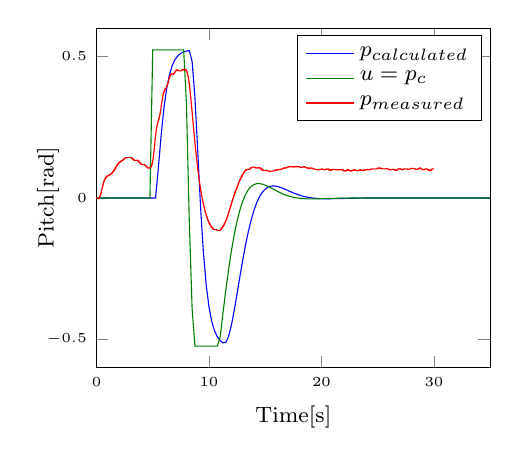
\begin{tikzpicture}

\begin{axis}[%
width = 5cm,
at={(0.772in,0.516in)},
scale only axis,
xmin=0,
xmax=35,
xlabel={\footnotesize{Time[s]}},
ymin=-0.6,
ymax=0.6,
ylabel={\footnotesize{Pitch[rad]}},
axis background/.style={fill=white},
ticklabel style = {font=\tiny},
ylabel shift = -0.4cm,
legend style={legend cell align=left, align=left, draw=black, font = \footnotesize}
]
\addplot [color=blue]
  table[row sep=crcr]{%
0	0\\
5.25	0\\
5.5	0.106028752059018\\
5.75	0.222660379323436\\
6	0.318881471816432\\
6.25	0.389443606311282\\
6.5	0.437955073776585\\
6.75	0.469972642303759\\
7	0.490517248775326\\
7.25	0.503431001414491\\
7.5	0.511421385860146\\
7.75	0.516304398576693\\
8	0.51925862126776\\
8.25	0.521031154883602\\
8.5	0.48281092448925\\
8.75	0.356835413424932\\
9	0.16746103620185\\
9.25	-0.029764323976778\\
9.5	-0.189426471823346\\
9.75	-0.305394163031721\\
10	-0.38466082364566\\
10.25	-0.436773923734016\\
10.5	-0.470120168998655\\
10.75	-0.491036826023787\\
11	-0.503957909562715\\
11.25	-0.511843812705287\\
11.5	-0.509873884142209\\
11.75	-0.488044662546464\\
12	-0.448317562621909\\
12.25	-0.396302164538795\\
12.5	-0.337841222779957\\
12.75	-0.277797273112583\\
13	-0.219777579686458\\
13.25	-0.166223560264768\\
13.5	-0.118614773398846\\
13.75	-0.0776857142937644\\
14	-0.0436189313642856\\
14.25	-0.0162051508067833\\
14.5	0.00502861402445376\\
14.75	0.0207188048747398\\
15	0.031588306158298\\
15.25	0.0383885280986647\\
15.5	0.0418570731669092\\
15.75	0.0426880532728404\\
16	0.0415125969082339\\
16.25	0.0388874620685513\\
16.5	0.0352899784891676\\
17	0.0266922100468321\\
17.5	0.0180198945219203\\
18	0.0105668753688875\\
18.25	0.00748975446614963\\
18.5	0.00487711066792684\\
18.75	0.00272129828724843\\
19.25	-0.000331544740703293\\
19.75	-0.00198440960986801\\
20.25	-0.00261678996314174\\
21	-0.0024224649675233\\
24	2.24482925688108e-05\\
26	0.000136959231831213\\
34.75	0\\
35	0\\
};
\addlegendentry{$p_{\text{calculated}}$}

\addplot [color=black!50!green]
  table[row sep=crcr]{%
0	0\\
4.75	0\\
5	0.523598775599787\\
7.75	0.52359877559762\\
8	0.329641417534724\\
8.25	-0.0821959464738384\\
8.5	-0.390161056333724\\
8.75	-0.523598771544535\\
10.75	-0.523598775597527\\
11	-0.490335594119088\\
11.25	-0.405017991769768\\
11.5	-0.324470537154674\\
11.75	-0.250796820123448\\
12	-0.18530817027365\\
12.25	-0.128658433716602\\
12.5	-0.0809755513755803\\
12.75	-0.0419846801294881\\
13	-0.0111188887049423\\
13.25	0.0123847380981346\\
13.5	0.0294043723738397\\
13.75	0.0408678771361295\\
14	0.0477014971566447\\
14.25	0.0507914633520414\\
14.5	0.0509569211776792\\
14.75	0.0489324928353057\\
15	0.0453587894876932\\
15.25	0.0407792717979873\\
16.5	0.0154955264225762\\
16.75	0.0114346776197891\\
17	0.00792142596289125\\
17.25	0.00496501724260412\\
17.5	0.00254888290762523\\
17.75	0.000637883187366128\\
18.25	-0.00186603813065034\\
18.75	-0.00298985344670655\\
19.25	-0.00318120213370321\\
20	-0.00253751205629271\\
22	-0.000305082336403473\\
23.5	0.000186665800157471\\
28.75	-1.13083054031904e-07\\
35	0\\
};
\addlegendentry{$u = p_c$}

\addplot [color=red]
  table[row sep=crcr]{%
0	0\\
0.0159999999999982	0\\
0.0180000000000007	-0.00153398078788669\\
0.186	-0.00153398078788669\\
0.187999999999999	0\\
0.23	0\\
0.231999999999999	0.00153398078788669\\
0.257999999999999	0.00153398078788669\\
0.260000000000002	0.00306796157576983\\
0.283999999999999	0.00306796157576983\\
0.286000000000001	0.00460194236365652\\
0.300000000000001	0.00460194236365652\\
0.302	0.00613592315154321\\
0.321999999999999	0.00613592315154321\\
0.324000000000002	0.0076699039394299\\
0.334	0.0076699039394299\\
0.335999999999999	0.00920388472731304\\
0.347999999999999	0.00920388472731304\\
0.350000000000001	0.0107378655151997\\
0.361999999999998	0.0107378655151997\\
0.364000000000001	0.0122718463030864\\
0.373999999999999	0.0122718463030864\\
0.376000000000001	0.0138058270909696\\
0.379999999999999	0.0138058270909696\\
0.382000000000001	0.0153398078788562\\
0.391999999999999	0.0153398078788562\\
0.393999999999998	0.0168737886667429\\
0.405999999999999	0.0168737886667429\\
0.408000000000001	0.0184077694546261\\
0.417999999999999	0.0184077694546261\\
0.420000000000002	0.0199417502425128\\
0.422000000000001	0.0199417502425128\\
0.423999999999999	0.0214757310303995\\
0.434000000000001	0.0214757310303995\\
0.436	0.0230097118182861\\
0.446000000000002	0.0230097118182861\\
0.448	0.0245436926061693\\
0.449999999999999	0.0245436926061693\\
0.452000000000002	0.026077673394056\\
0.462	0.026077673394056\\
0.463999999999999	0.0276116541819427\\
0.469999999999999	0.0276116541819427\\
0.472000000000001	0.0291456349698258\\
0.48	0.0291456349698258\\
0.481999999999999	0.0306796157577125\\
0.486000000000001	0.0306796157577125\\
0.488	0.0322135965455992\\
0.498000000000001	0.0322135965455992\\
0.5	0.0337475773334859\\
0.507999999999999	0.0337475773334859\\
0.510000000000002	0.035281558121369\\
0.513999999999999	0.035281558121369\\
0.516000000000002	0.0368155389092557\\
0.524000000000001	0.0368155389092557\\
0.526	0.0383495196971424\\
0.530000000000001	0.0383495196971424\\
0.532	0.0398835004850255\\
0.539999999999999	0.0398835004850255\\
0.542000000000002	0.0414174812729122\\
0.550000000000001	0.0414174812729122\\
0.552	0.0429514620607989\\
0.558	0.0429514620607989\\
0.559999999999999	0.0444854428486821\\
0.57	0.0444854428486821\\
0.571999999999999	0.0460194236365687\\
0.577999999999999	0.0460194236365687\\
0.579999999999998	0.0475534044244554\\
0.588000000000001	0.0475534044244554\\
0.59	0.0490873852123421\\
0.600000000000001	0.0490873852123421\\
0.602	0.0506213660002253\\
0.609999999999999	0.0506213660002253\\
0.611999999999998	0.052155346788112\\
0.617999999999999	0.052155346788112\\
0.620000000000001	0.0536893275759986\\
0.629999999999999	0.0536893275759986\\
0.632000000000001	0.0552233083638818\\
0.643999999999998	0.0552233083638818\\
0.646000000000001	0.0567572891517685\\
0.654	0.0567572891517685\\
0.655999999999999	0.0582912699396552\\
0.667999999999999	0.0582912699396552\\
0.670000000000002	0.0598252507275383\\
0.681999999999999	0.0598252507275383\\
0.684000000000001	0.061359231515425\\
0.698	0.061359231515425\\
0.699999999999999	0.0628932123033117\\
0.712	0.0628932123033117\\
0.713999999999999	0.0644271930911984\\
0.725999999999999	0.0644271930911984\\
0.728000000000002	0.0659611738790815\\
0.745999999999999	0.0659611738790815\\
0.748000000000001	0.0674951546669682\\
0.766000000000002	0.0674951546669682\\
0.768000000000001	0.0690291354548549\\
0.788	0.0690291354548549\\
0.789999999999999	0.070563116242738\\
0.809999999999999	0.070563116242738\\
0.812000000000001	0.0720970970306247\\
0.841999999999999	0.0720970970306247\\
0.844000000000001	0.0736310778185114\\
0.873999999999999	0.0736310778185114\\
0.876000000000001	0.0751650586063981\\
0.916	0.0751650586063981\\
0.917999999999999	0.0766990393942812\\
0.966000000000001	0.0766990393942812\\
0.968	0.0782330201821679\\
1.044	0.0782330201821679\\
1.046	0.0797670009700546\\
1.122	0.0797670009700546\\
1.124	0.0813009817579378\\
1.194	0.0813009817579378\\
1.196	0.0828349625458245\\
1.254	0.0828349625458245\\
1.256	0.0843689433337111\\
1.304	0.0843689433337111\\
1.306	0.0859029241215943\\
1.344	0.0859029241215943\\
1.346	0.087436904909481\\
1.382	0.087436904909481\\
1.384	0.0889708856973677\\
1.412	0.0889708856973677\\
1.414	0.0905048664852544\\
1.442	0.0905048664852544\\
1.444	0.0920388472731375\\
1.472	0.0920388472731375\\
1.474	0.0935728280610242\\
1.502	0.0935728280610242\\
1.504	0.0951068088489109\\
1.528	0.0951068088489109\\
1.53	0.096640789636794\\
1.556	0.096640789636794\\
1.558	0.0981747704246807\\
1.58	0.0981747704246807\\
1.582	0.0997087512125674\\
1.604	0.0997087512125674\\
1.606	0.101242732000454\\
1.624	0.101242732000454\\
1.626	0.102776712788337\\
1.648	0.102776712788337\\
1.65	0.104310693576224\\
1.672	0.104310693576224\\
1.674	0.105844674364111\\
1.7	0.105844674364111\\
1.702	0.107378655151994\\
1.72	0.107378655151994\\
1.722	0.10891263593988\\
1.742	0.10891263593988\\
1.744	0.110446616727767\\
1.762	0.110446616727767\\
1.764	0.11198059751565\\
1.784	0.11198059751565\\
1.786	0.113514578303537\\
1.804	0.113514578303537\\
1.806	0.115048559091424\\
1.826	0.115048559091424\\
1.828	0.11658253987931\\
1.854	0.11658253987931\\
1.856	0.118116520667193\\
1.88	0.118116520667193\\
1.882	0.11965050145508\\
1.904	0.11965050145508\\
1.906	0.121184482242967\\
1.94	0.121184482242967\\
1.942	0.12271846303085\\
1.978	0.12271846303085\\
1.98	0.124252443818737\\
2.018	0.124252443818737\\
2.02	0.125786424606623\\
2.06	0.125786424606623\\
2.062	0.127320405394507\\
2.122	0.127320405394507\\
2.124	0.128854386182393\\
2.184	0.128854386182393\\
2.186	0.13038836697028\\
2.238	0.13038836697028\\
2.24	0.131922347758167\\
2.284	0.131922347758167\\
2.286	0.13345632854605\\
2.346	0.13345632854605\\
2.348	0.134990309333936\\
2.394	0.134990309333936\\
2.396	0.136524290121823\\
2.44	0.136524290121823\\
2.442	0.138058270909706\\
2.476	0.138058270909706\\
2.478	0.139592251697593\\
2.528	0.139592251697593\\
2.53	0.14112623248548\\
2.58	0.14112623248548\\
2.582	0.142660213273366\\
3.122	0.142660213273366\\
3.124	0.14112623248548\\
3.166	0.14112623248548\\
3.168	0.139592251697593\\
3.208	0.139592251697593\\
3.21	0.138058270909706\\
3.244	0.138058270909706\\
3.246	0.136524290121823\\
3.28	0.136524290121823\\
3.282	0.134990309333936\\
3.332	0.134990309333936\\
3.334	0.13345632854605\\
3.654	0.13345632854605\\
3.656	0.131922347758167\\
3.7	0.131922347758167\\
3.702	0.13038836697028\\
3.734	0.13038836697028\\
3.736	0.128854386182393\\
3.776	0.128854386182393\\
3.778	0.127320405394507\\
3.806	0.127320405394507\\
3.808	0.125786424606623\\
3.846	0.125786424606623\\
3.848	0.124252443818737\\
3.878	0.124252443818737\\
3.88	0.12271846303085\\
3.908	0.12271846303085\\
3.91	0.121184482242967\\
3.95	0.121184482242967\\
3.952	0.11965050145508\\
4.008	0.11965050145508\\
4.01	0.118116520667193\\
4.258	0.118116520667193\\
4.26	0.11658253987931\\
4.33	0.11658253987931\\
4.332	0.115048559091424\\
4.384	0.115048559091424\\
4.386	0.113514578303537\\
4.416	0.113514578303537\\
4.418	0.11198059751565\\
4.454	0.11198059751565\\
4.456	0.110446616727767\\
4.482	0.110446616727767\\
4.484	0.10891263593988\\
4.518	0.10891263593988\\
4.52	0.107378655151994\\
4.56	0.107378655151994\\
4.562	0.105844674364111\\
4.754	0.105844674364111\\
4.756	0.107378655151994\\
4.798	0.107378655151994\\
4.8	0.10891263593988\\
4.836	0.10891263593988\\
4.838	0.110446616727767\\
4.862	0.110446616727767\\
4.864	0.11198059751565\\
4.88	0.11198059751565\\
4.882	0.113514578303537\\
4.896	0.113514578303537\\
4.898	0.115048559091424\\
4.91	0.115048559091424\\
4.912	0.11658253987931\\
4.922	0.11658253987931\\
4.924	0.118116520667193\\
4.934	0.118116520667193\\
4.936	0.11965050145508\\
4.944	0.11965050145508\\
4.946	0.121184482242967\\
4.954	0.121184482242967\\
4.956	0.12271846303085\\
4.964	0.12271846303085\\
4.966	0.124252443818737\\
4.972	0.124252443818737\\
4.974	0.125786424606623\\
4.978	0.125786424606623\\
4.98	0.127320405394507\\
4.986	0.127320405394507\\
4.988	0.128854386182393\\
4.994	0.128854386182393\\
4.996	0.13038836697028\\
5	0.13038836697028\\
5.002	0.131922347758167\\
5.006	0.131922347758167\\
5.008	0.13345632854605\\
5.014	0.13345632854605\\
5.016	0.134990309333936\\
5.018	0.134990309333936\\
5.02	0.136524290121823\\
5.026	0.136524290121823\\
5.028	0.138058270909706\\
5.03	0.138058270909706\\
5.032	0.139592251697593\\
5.036	0.139592251697593\\
5.038	0.14112623248548\\
5.042	0.14112623248548\\
5.044	0.142660213273366\\
5.048	0.142660213273366\\
5.05	0.144194194061249\\
5.052	0.144194194061249\\
5.054	0.145728174849136\\
5.058	0.145728174849136\\
5.06	0.147262155637023\\
5.062	0.147262155637023\\
5.064	0.148796136424906\\
5.068	0.148796136424906\\
5.07	0.150330117212793\\
5.072	0.150330117212793\\
5.074	0.151864098000679\\
5.076	0.151864098000679\\
5.078	0.153398078788562\\
5.082	0.153398078788562\\
5.084	0.154932059576449\\
5.086	0.154932059576449\\
5.088	0.156466040364336\\
5.09	0.156466040364336\\
5.092	0.158000021152223\\
5.094	0.158000021152223\\
5.096	0.159534001940106\\
5.098	0.159534001940106\\
5.1	0.161067982727992\\
5.104	0.161067982727992\\
5.106	0.162601963515879\\
5.108	0.162601963515879\\
5.11	0.164135944303762\\
5.112	0.164135944303762\\
5.114	0.165669925091649\\
5.116	0.165669925091649\\
5.118	0.167203905879536\\
5.12	0.167203905879536\\
5.122	0.168737886667422\\
5.124	0.168737886667422\\
5.126	0.170271867455305\\
5.128	0.170271867455305\\
5.13	0.171805848243192\\
5.132	0.171805848243192\\
5.134	0.173339829031079\\
5.136	0.173339829031079\\
5.138	0.174873809818962\\
5.14	0.174873809818962\\
5.142	0.176407790606849\\
5.144	0.176407790606849\\
5.146	0.177941771394735\\
5.148	0.177941771394735\\
5.15	0.179475752182618\\
5.152	0.179475752182618\\
5.154	0.181009732970505\\
5.156	0.181009732970505\\
5.158	0.182543713758392\\
5.16	0.182543713758392\\
5.162	0.184077694546279\\
5.164	0.184077694546279\\
5.166	0.185611675334162\\
5.168	0.185611675334162\\
5.172	0.188679636909935\\
5.174	0.188679636909935\\
5.176	0.190213617697818\\
5.178	0.190213617697818\\
5.18	0.191747598485705\\
5.182	0.191747598485705\\
5.184	0.193281579273592\\
5.186	0.193281579273592\\
5.188	0.194815560061475\\
5.19	0.194815560061475\\
5.192	0.196349540849361\\
5.194	0.196349540849361\\
5.196	0.197883521637248\\
5.198	0.197883521637248\\
5.2	0.199417502425135\\
5.202	0.199417502425135\\
5.204	0.200951483213018\\
5.206	0.200951483213018\\
5.208	0.202485464000905\\
5.21	0.202485464000905\\
5.212	0.204019444788791\\
5.214	0.204019444788791\\
5.216	0.205553425576674\\
5.218	0.205553425576674\\
5.22	0.207087406364561\\
5.222	0.207087406364561\\
5.224	0.208621387152448\\
5.226	0.208621387152448\\
5.228	0.210155367940335\\
5.23	0.210155367940335\\
5.232	0.211689348728218\\
5.234	0.211689348728218\\
5.236	0.213223329516104\\
5.24	0.213223329516104\\
5.242	0.214757310303991\\
5.244	0.214757310303991\\
5.246	0.216291291091874\\
5.248	0.216291291091874\\
5.25	0.217825271879761\\
5.252	0.217825271879761\\
5.254	0.219359252667648\\
5.256	0.219359252667648\\
5.258	0.220893233455531\\
5.26	0.220893233455531\\
5.262	0.222427214243417\\
5.264	0.222427214243417\\
5.266	0.223961195031304\\
5.27	0.223961195031304\\
5.272	0.225495175819191\\
5.274	0.225495175819191\\
5.276	0.227029156607074\\
5.278	0.227029156607074\\
5.28	0.228563137394961\\
5.282	0.228563137394961\\
5.284	0.230097118182847\\
5.288	0.230097118182847\\
5.29	0.23163109897073\\
5.294	0.23163109897073\\
5.296	0.233165079758617\\
5.298	0.233165079758617\\
5.3	0.234699060546504\\
5.302	0.234699060546504\\
5.304	0.23623304133439\\
5.308	0.23623304133439\\
5.31	0.237767022122274\\
5.312	0.237767022122274\\
5.314	0.23930100291016\\
5.318	0.23930100291016\\
5.32	0.240834983698047\\
5.324	0.240834983698047\\
5.326	0.24236896448593\\
5.33	0.24236896448593\\
5.332	0.243902945273817\\
5.336	0.243902945273817\\
5.338	0.245436926061704\\
5.342	0.245436926061704\\
5.344	0.246970906849587\\
5.35	0.246970906849587\\
5.352	0.248504887637473\\
5.354	0.248504887637473\\
5.356	0.25003886842536\\
5.362	0.25003886842536\\
5.364	0.251572849213247\\
5.368	0.251572849213247\\
5.37	0.25310683000113\\
5.376	0.25310683000113\\
5.378	0.254640810789017\\
5.382	0.254640810789017\\
5.384	0.256174791576903\\
5.392	0.256174791576903\\
5.394	0.257708772364786\\
5.4	0.257708772364786\\
5.402	0.259242753152673\\
5.408	0.259242753152673\\
5.41	0.26077673394056\\
5.418	0.26077673394056\\
5.42	0.262310714728443\\
5.428	0.262310714728443\\
5.43	0.26384469551633\\
5.436	0.26384469551633\\
5.438	0.265378676304216\\
5.448	0.265378676304216\\
5.45	0.266912657092103\\
5.458	0.266912657092103\\
5.46	0.268446637879986\\
5.47	0.268446637879986\\
5.472	0.269980618667873\\
5.48	0.269980618667873\\
5.482	0.27151459945576\\
5.492	0.27151459945576\\
5.494	0.273048580243643\\
5.504	0.273048580243643\\
5.506	0.274582561031529\\
5.518	0.274582561031529\\
5.52	0.276116541819416\\
5.528	0.276116541819416\\
5.53	0.277650522607303\\
5.538	0.277650522607303\\
5.54	0.279184503395186\\
5.548	0.279184503395186\\
5.55	0.280718484183073\\
5.56	0.280718484183073\\
5.562	0.282252464970959\\
5.57	0.282252464970959\\
5.572	0.283786445758842\\
5.58	0.283786445758842\\
5.582	0.285320426546729\\
5.588	0.285320426546729\\
5.59	0.286854407334616\\
5.598	0.286854407334616\\
5.6	0.288388388122499\\
5.608	0.288388388122499\\
5.61	0.289922368910386\\
5.616	0.289922368910386\\
5.618	0.291456349698272\\
5.624	0.291456349698272\\
5.626	0.292990330486159\\
5.632	0.292990330486159\\
5.634	0.294524311274042\\
5.64	0.294524311274042\\
5.642	0.296058292061929\\
5.646	0.296058292061929\\
5.648	0.297592272849815\\
5.654	0.297592272849815\\
5.656	0.299126253637699\\
5.66	0.299126253637699\\
5.662	0.300660234425585\\
5.668	0.300660234425585\\
5.67	0.302194215213472\\
5.674	0.302194215213472\\
5.676	0.303728196001359\\
5.682	0.303728196001359\\
5.684	0.305262176789242\\
5.688	0.305262176789242\\
5.69	0.306796157577129\\
5.696	0.306796157577129\\
5.698	0.308330138365015\\
5.7	0.308330138365015\\
5.702	0.309864119152898\\
5.708	0.309864119152898\\
5.71	0.311398099940785\\
5.714	0.311398099940785\\
5.716	0.312932080728672\\
5.72	0.312932080728672\\
5.722	0.314466061516555\\
5.726	0.314466061516555\\
5.728	0.316000042304442\\
5.73	0.316000042304442\\
5.732	0.317534023092328\\
5.738	0.317534023092328\\
5.74	0.319068003880215\\
5.742	0.319068003880215\\
5.744	0.320601984668098\\
5.748	0.320601984668098\\
5.75	0.322135965455985\\
5.754	0.322135965455985\\
5.756	0.323669946243871\\
5.758	0.323669946243871\\
5.76	0.325203927031755\\
5.764	0.325203927031755\\
5.766	0.326737907819641\\
5.77	0.326737907819641\\
5.772	0.328271888607528\\
5.776	0.328271888607528\\
5.778	0.329805869395411\\
5.782	0.329805869395411\\
5.784	0.331339850183298\\
5.786	0.331339850183298\\
5.788	0.332873830971185\\
5.792	0.332873830971185\\
5.794	0.334407811759071\\
5.798	0.334407811759071\\
5.8	0.335941792546954\\
5.804	0.335941792546954\\
5.806	0.337475773334841\\
5.81	0.337475773334841\\
5.812	0.339009754122728\\
5.814	0.339009754122728\\
5.816	0.340543734910611\\
5.82	0.340543734910611\\
5.822	0.342077715698498\\
5.828	0.342077715698498\\
5.83	0.343611696486384\\
5.832	0.343611696486384\\
5.834	0.345145677274271\\
5.838	0.345145677274271\\
5.84	0.346679658062154\\
5.844	0.346679658062154\\
5.846	0.348213638850041\\
5.85	0.348213638850041\\
5.852	0.349747619637927\\
5.858	0.349747619637927\\
5.86	0.351281600425811\\
5.862	0.351281600425811\\
5.864	0.352815581213697\\
5.87	0.352815581213697\\
5.872	0.354349562001584\\
5.874	0.354349562001584\\
5.876	0.355883542789467\\
5.882	0.355883542789467\\
5.884	0.357417523577354\\
5.888	0.357417523577354\\
5.89	0.35895150436524\\
5.896	0.35895150436524\\
5.898	0.360485485153127\\
5.902	0.360485485153127\\
5.904	0.36201946594101\\
5.912	0.36201946594101\\
5.914	0.363553446728897\\
5.918	0.363553446728897\\
5.92	0.365087427516784\\
5.926	0.365087427516784\\
5.928	0.366621408304667\\
5.936	0.366621408304667\\
5.938	0.368155389092554\\
5.944	0.368155389092554\\
5.946	0.36968936988044\\
5.954	0.36968936988044\\
5.956	0.371223350668327\\
5.966	0.371223350668327\\
5.968	0.37275733145621\\
5.978	0.37275733145621\\
5.98	0.374291312244097\\
5.992	0.374291312244097\\
5.994	0.375825293031983\\
6.008	0.375825293031983\\
6.01	0.377359273819867\\
6.022	0.377359273819867\\
6.024	0.378893254607753\\
6.038	0.378893254607753\\
6.04	0.38042723539564\\
6.058	0.38042723539564\\
6.06	0.381961216183523\\
6.084	0.381961216183523\\
6.086	0.38349519697141\\
6.11	0.38349519697141\\
6.112	0.385029177759296\\
6.14	0.385029177759296\\
6.142	0.386563158547183\\
6.168	0.386563158547183\\
6.17	0.388097139335066\\
6.186	0.388097139335066\\
6.188	0.389631120122953\\
6.21	0.389631120122953\\
6.212	0.39116510091084\\
6.226	0.39116510091084\\
6.228	0.392699081698723\\
6.242	0.392699081698723\\
6.244	0.394233062486609\\
6.258	0.394233062486609\\
6.26	0.395767043274496\\
6.272	0.395767043274496\\
6.274	0.397301024062379\\
6.286	0.397301024062379\\
6.288	0.398835004850266\\
6.3	0.398835004850266\\
6.302	0.400368985638153\\
6.312	0.400368985638153\\
6.314	0.401902966426039\\
6.322	0.401902966426039\\
6.324	0.403436947213923\\
6.334	0.403436947213923\\
6.336	0.404970928001809\\
6.346	0.404970928001809\\
6.348	0.406504908789696\\
6.358	0.406504908789696\\
6.36	0.408038889577579\\
6.366	0.408038889577579\\
6.368	0.409572870365466\\
6.378	0.409572870365466\\
6.38	0.411106851153352\\
6.39	0.411106851153352\\
6.392	0.412640831941239\\
6.4	0.412640831941239\\
6.402	0.414174812729122\\
6.408	0.414174812729122\\
6.41	0.415708793517009\\
6.42	0.415708793517009\\
6.422	0.417242774304896\\
6.432	0.417242774304896\\
6.434	0.418776755092779\\
6.442	0.418776755092779\\
6.444	0.420310735880665\\
6.452	0.420310735880665\\
6.454	0.421844716668552\\
6.464	0.421844716668552\\
6.466	0.423378697456435\\
6.476	0.423378697456435\\
6.478	0.424912678244322\\
6.49	0.424912678244322\\
6.492	0.426446659032209\\
6.5	0.426446659032209\\
6.502	0.427980639820095\\
6.512	0.427980639820095\\
6.514	0.429514620607979\\
6.526	0.429514620607979\\
6.528	0.431048601395865\\
6.544	0.431048601395865\\
6.546	0.432582582183752\\
6.56	0.432582582183752\\
6.562	0.434116562971635\\
6.586	0.434116562971635\\
6.588	0.435650543759522\\
6.616	0.435650543759522\\
6.618	0.437184524547408\\
6.692	0.437184524547408\\
6.694	0.438718505335295\\
6.696	0.438718505335295\\
6.698	0.437184524547408\\
6.704	0.437184524547408\\
6.706	0.438718505335295\\
6.71	0.438718505335295\\
6.712	0.437184524547408\\
6.828	0.437184524547408\\
6.83	0.438718505335295\\
6.872	0.438718505335295\\
6.874	0.440252486123178\\
6.908	0.440252486123178\\
6.91	0.441786466911065\\
6.938	0.441786466911065\\
6.94	0.443320447698952\\
6.966	0.443320447698952\\
6.968	0.444854428486835\\
6.984	0.444854428486835\\
6.986	0.446388409274721\\
7.012	0.446388409274721\\
7.014	0.447922390062608\\
7.04	0.447922390062608\\
7.042	0.449456370850491\\
7.082	0.449456370850491\\
7.084	0.450990351638378\\
7.126	0.450990351638378\\
7.128	0.452524332426265\\
7.208	0.452524332426265\\
7.21	0.450990351638378\\
7.214	0.450990351638378\\
7.216	0.452524332426265\\
7.218	0.452524332426265\\
7.22	0.450990351638378\\
7.28	0.450990351638378\\
7.282	0.449456370850491\\
7.54	0.449456370850491\\
7.542	0.450990351638378\\
7.608	0.450990351638378\\
7.61	0.452524332426265\\
7.668	0.452524332426265\\
7.67	0.454058313214151\\
7.91	0.454058313214151\\
7.912	0.452524332426265\\
7.956	0.452524332426265\\
7.958	0.450990351638378\\
7.98	0.450990351638378\\
7.982	0.449456370850491\\
8.004	0.449456370850491\\
8.006	0.447922390062608\\
8.02	0.447922390062608\\
8.022	0.446388409274721\\
8.036	0.446388409274721\\
8.038	0.444854428486835\\
8.05	0.444854428486835\\
8.052	0.443320447698952\\
8.064	0.443320447698952\\
8.066	0.441786466911065\\
8.076	0.441786466911065\\
8.078	0.440252486123178\\
8.09	0.440252486123178\\
8.092	0.438718505335295\\
8.096	0.438718505335295\\
8.098	0.437184524547408\\
8.108	0.437184524547408\\
8.11	0.435650543759522\\
8.118	0.435650543759522\\
8.12	0.434116562971635\\
8.124	0.434116562971635\\
8.126	0.432582582183752\\
8.134	0.432582582183752\\
8.136	0.431048601395865\\
8.142	0.431048601395865\\
8.144	0.429514620607979\\
8.15	0.429514620607979\\
8.152	0.427980639820095\\
8.156	0.427980639820095\\
8.158	0.426446659032209\\
8.164	0.426446659032209\\
8.166	0.424912678244322\\
8.172	0.424912678244322\\
8.174	0.423378697456435\\
8.178	0.423378697456435\\
8.18	0.421844716668552\\
8.184	0.421844716668552\\
8.186	0.420310735880665\\
8.19	0.420310735880665\\
8.192	0.418776755092779\\
8.196	0.418776755092779\\
8.198	0.417242774304896\\
8.204	0.417242774304896\\
8.206	0.415708793517009\\
8.208	0.415708793517009\\
8.21	0.414174812729122\\
8.214	0.414174812729122\\
8.216	0.412640831941239\\
8.22	0.412640831941239\\
8.222	0.411106851153352\\
8.224	0.411106851153352\\
8.226	0.409572870365466\\
8.23	0.409572870365466\\
8.232	0.408038889577579\\
8.236	0.408038889577579\\
8.238	0.406504908789696\\
8.24	0.406504908789696\\
8.242	0.404970928001809\\
8.246	0.404970928001809\\
8.248	0.403436947213923\\
8.25	0.403436947213923\\
8.252	0.401902966426039\\
8.256	0.401902966426039\\
8.258	0.400368985638153\\
8.26	0.400368985638153\\
8.262	0.398835004850266\\
8.266	0.398835004850266\\
8.268	0.397301024062379\\
8.27	0.397301024062379\\
8.272	0.395767043274496\\
8.274	0.395767043274496\\
8.276	0.394233062486609\\
8.28	0.394233062486609\\
8.282	0.392699081698723\\
8.284	0.392699081698723\\
8.286	0.39116510091084\\
8.288	0.39116510091084\\
8.29	0.389631120122953\\
8.292	0.389631120122953\\
8.294	0.388097139335066\\
8.298	0.388097139335066\\
8.3	0.386563158547183\\
8.302	0.386563158547183\\
8.304	0.385029177759296\\
8.306	0.385029177759296\\
8.308	0.38349519697141\\
8.31	0.38349519697141\\
8.312	0.381961216183523\\
8.314	0.381961216183523\\
8.316	0.38042723539564\\
8.318	0.38042723539564\\
8.32	0.378893254607753\\
8.322	0.378893254607753\\
8.324	0.377359273819867\\
8.326	0.377359273819867\\
8.328	0.375825293031983\\
8.33	0.375825293031983\\
8.332	0.374291312244097\\
8.334	0.374291312244097\\
8.336	0.37275733145621\\
8.338	0.37275733145621\\
8.34	0.371223350668327\\
8.342	0.371223350668327\\
8.344	0.36968936988044\\
8.346	0.36968936988044\\
8.348	0.368155389092554\\
8.35	0.368155389092554\\
8.352	0.366621408304667\\
8.354	0.366621408304667\\
8.356	0.365087427516784\\
8.358	0.365087427516784\\
8.362	0.36201946594101\\
8.364	0.36201946594101\\
8.366	0.360485485153127\\
8.37	0.360485485153127\\
8.374	0.357417523577354\\
8.376	0.357417523577354\\
8.378	0.355883542789467\\
8.38	0.355883542789467\\
8.382	0.354349562001584\\
8.384	0.354349562001584\\
8.386	0.352815581213697\\
8.388	0.352815581213697\\
8.392	0.349747619637927\\
8.394	0.349747619637927\\
8.396	0.348213638850041\\
8.4	0.348213638850041\\
8.404	0.345145677274271\\
8.406	0.345145677274271\\
8.408	0.343611696486384\\
8.41	0.343611696486384\\
8.412	0.342077715698498\\
8.414	0.342077715698498\\
8.418	0.339009754122728\\
8.42	0.339009754122728\\
8.422	0.337475773334841\\
8.424	0.337475773334841\\
8.426	0.335941792546954\\
8.428	0.335941792546954\\
8.432	0.332873830971185\\
8.434	0.332873830971185\\
8.436	0.331339850183298\\
8.438	0.331339850183298\\
8.44	0.329805869395411\\
8.442	0.329805869395411\\
8.444	0.328271888607528\\
8.446	0.328271888607528\\
8.45	0.325203927031755\\
8.452	0.325203927031755\\
8.454	0.323669946243871\\
8.456	0.323669946243871\\
8.458	0.322135965455985\\
8.46	0.322135965455985\\
8.464	0.319068003880215\\
8.466	0.319068003880215\\
8.468	0.317534023092328\\
8.47	0.317534023092328\\
8.472	0.316000042304442\\
8.474	0.316000042304442\\
8.478	0.312932080728672\\
8.48	0.312932080728672\\
8.482	0.311398099940785\\
8.484	0.311398099940785\\
8.486	0.309864119152898\\
8.488	0.309864119152898\\
8.492	0.306796157577129\\
8.494	0.306796157577129\\
8.496	0.305262176789242\\
8.498	0.305262176789242\\
8.5	0.303728196001359\\
8.502	0.303728196001359\\
8.506	0.300660234425585\\
8.508	0.300660234425585\\
8.51	0.299126253637699\\
8.512	0.299126253637699\\
8.516	0.296058292061929\\
8.518	0.296058292061929\\
8.522	0.292990330486159\\
8.524	0.292990330486159\\
8.526	0.291456349698272\\
8.528	0.291456349698272\\
8.53	0.289922368910386\\
8.532	0.289922368910386\\
8.536	0.286854407334616\\
8.538	0.286854407334616\\
8.54	0.285320426546729\\
8.542	0.285320426546729\\
8.544	0.283786445758842\\
8.546	0.283786445758842\\
8.55	0.280718484183073\\
8.552	0.280718484183073\\
8.554	0.279184503395186\\
8.556	0.279184503395186\\
8.558	0.277650522607303\\
8.56	0.277650522607303\\
8.564	0.274582561031529\\
8.566	0.274582561031529\\
8.568	0.273048580243643\\
8.57	0.273048580243643\\
8.572	0.27151459945576\\
8.574	0.27151459945576\\
8.578	0.268446637879986\\
8.58	0.268446637879986\\
8.582	0.266912657092103\\
8.584	0.266912657092103\\
8.586	0.265378676304216\\
8.588	0.265378676304216\\
8.592	0.262310714728443\\
8.594	0.262310714728443\\
8.596	0.26077673394056\\
8.598	0.26077673394056\\
8.602	0.257708772364786\\
8.604	0.257708772364786\\
8.606	0.256174791576903\\
8.608	0.256174791576903\\
8.61	0.254640810789017\\
8.612	0.254640810789017\\
8.616	0.251572849213247\\
8.618	0.251572849213247\\
8.62	0.25003886842536\\
8.622	0.25003886842536\\
8.624	0.248504887637473\\
8.626	0.248504887637473\\
8.628	0.246970906849587\\
8.63	0.246970906849587\\
8.634	0.243902945273817\\
8.636	0.243902945273817\\
8.638	0.24236896448593\\
8.64	0.24236896448593\\
8.642	0.240834983698047\\
8.644	0.240834983698047\\
8.648	0.237767022122274\\
8.65	0.237767022122274\\
8.652	0.23623304133439\\
8.654	0.23623304133439\\
8.656	0.234699060546504\\
8.658	0.234699060546504\\
8.66	0.233165079758617\\
8.662	0.233165079758617\\
8.664	0.23163109897073\\
8.666	0.23163109897073\\
8.67	0.228563137394961\\
8.672	0.228563137394961\\
8.674	0.227029156607074\\
8.676	0.227029156607074\\
8.678	0.225495175819191\\
8.68	0.225495175819191\\
8.682	0.223961195031304\\
8.684	0.223961195031304\\
8.688	0.220893233455531\\
8.69	0.220893233455531\\
8.692	0.219359252667648\\
8.694	0.219359252667648\\
8.696	0.217825271879761\\
8.698	0.217825271879761\\
8.7	0.216291291091874\\
8.702	0.216291291091874\\
8.704	0.214757310303991\\
8.706	0.214757310303991\\
8.708	0.213223329516104\\
8.71	0.213223329516104\\
8.712	0.211689348728218\\
8.714	0.211689348728218\\
8.718	0.208621387152448\\
8.72	0.208621387152448\\
8.722	0.207087406364561\\
8.724	0.207087406364561\\
8.726	0.205553425576674\\
8.728	0.205553425576674\\
8.73	0.204019444788791\\
8.732	0.204019444788791\\
8.734	0.202485464000905\\
8.736	0.202485464000905\\
8.738	0.200951483213018\\
8.74	0.200951483213018\\
8.742	0.199417502425135\\
8.744	0.199417502425135\\
8.746	0.197883521637248\\
8.748	0.197883521637248\\
8.75	0.196349540849361\\
8.752	0.196349540849361\\
8.754	0.194815560061475\\
8.756	0.194815560061475\\
8.758	0.193281579273592\\
8.76	0.193281579273592\\
8.762	0.191747598485705\\
8.764	0.191747598485705\\
8.766	0.190213617697818\\
8.768	0.190213617697818\\
8.77	0.188679636909935\\
8.772	0.188679636909935\\
8.776	0.185611675334162\\
8.78	0.185611675334162\\
8.782	0.184077694546279\\
8.784	0.184077694546279\\
8.786	0.182543713758392\\
8.788	0.182543713758392\\
8.792	0.179475752182618\\
8.796	0.179475752182618\\
8.798	0.177941771394735\\
8.8	0.177941771394735\\
8.804	0.174873809818962\\
8.806	0.174873809818962\\
8.808	0.173339829031079\\
8.81	0.173339829031079\\
8.812	0.171805848243192\\
8.816	0.171805848243192\\
8.82	0.168737886667422\\
8.822	0.168737886667422\\
8.824	0.167203905879536\\
8.828	0.167203905879536\\
8.83	0.165669925091649\\
8.832	0.165669925091649\\
8.836	0.162601963515879\\
8.84	0.162601963515879\\
8.842	0.161067982727992\\
8.844	0.161067982727992\\
8.846	0.159534001940106\\
8.848	0.159534001940106\\
8.85	0.158000021152223\\
8.852	0.158000021152223\\
8.854	0.156466040364336\\
8.856	0.156466040364336\\
8.858	0.154932059576449\\
8.86	0.154932059576449\\
8.862	0.153398078788562\\
8.864	0.153398078788562\\
8.866	0.151864098000679\\
8.868	0.151864098000679\\
8.87	0.150330117212793\\
8.872	0.150330117212793\\
8.874	0.148796136424906\\
8.876	0.148796136424906\\
8.878	0.147262155637023\\
8.88	0.147262155637023\\
8.882	0.145728174849136\\
8.886	0.145728174849136\\
8.888	0.144194194061249\\
8.89	0.144194194061249\\
8.892	0.142660213273366\\
8.894	0.142660213273366\\
8.896	0.14112623248548\\
8.898	0.14112623248548\\
8.9	0.139592251697593\\
8.902	0.139592251697593\\
8.904	0.138058270909706\\
8.906	0.138058270909706\\
8.908	0.136524290121823\\
8.91	0.136524290121823\\
8.912	0.134990309333936\\
8.914	0.134990309333936\\
8.916	0.13345632854605\\
8.918	0.13345632854605\\
8.92	0.131922347758167\\
8.922	0.131922347758167\\
8.924	0.13038836697028\\
8.926	0.13038836697028\\
8.928	0.128854386182393\\
8.932	0.128854386182393\\
8.934	0.127320405394507\\
8.936	0.127320405394507\\
8.938	0.125786424606623\\
8.94	0.125786424606623\\
8.942	0.124252443818737\\
8.944	0.124252443818737\\
8.946	0.12271846303085\\
8.948	0.12271846303085\\
8.95	0.121184482242967\\
8.952	0.121184482242967\\
8.954	0.11965050145508\\
8.958	0.11965050145508\\
8.96	0.118116520667193\\
8.962	0.118116520667193\\
8.964	0.11658253987931\\
8.966	0.11658253987931\\
8.968	0.115048559091424\\
8.97	0.115048559091424\\
8.972	0.113514578303537\\
8.974	0.113514578303537\\
8.976	0.11198059751565\\
8.98	0.11198059751565\\
8.982	0.110446616727767\\
8.984	0.110446616727767\\
8.986	0.10891263593988\\
8.988	0.10891263593988\\
8.99	0.107378655151994\\
8.992	0.107378655151994\\
8.994	0.105844674364111\\
8.998	0.105844674364111\\
9	0.104310693576224\\
9.002	0.104310693576224\\
9.004	0.102776712788337\\
9.006	0.102776712788337\\
9.008	0.101242732000454\\
9.01	0.101242732000454\\
9.012	0.0997087512125674\\
9.016	0.0997087512125674\\
9.018	0.0981747704246807\\
9.02	0.0981747704246807\\
9.022	0.096640789636794\\
9.024	0.096640789636794\\
9.026	0.0951068088489109\\
9.03	0.0951068088489109\\
9.032	0.0935728280610242\\
9.034	0.0935728280610242\\
9.036	0.0920388472731375\\
9.038	0.0920388472731375\\
9.04	0.0905048664852544\\
9.044	0.0905048664852544\\
9.046	0.0889708856973677\\
9.048	0.0889708856973677\\
9.05	0.087436904909481\\
9.054	0.087436904909481\\
9.056	0.0859029241215943\\
9.058	0.0859029241215943\\
9.06	0.0843689433337111\\
9.064	0.0843689433337111\\
9.066	0.0828349625458245\\
9.068	0.0828349625458245\\
9.07	0.0813009817579378\\
9.074	0.0813009817579378\\
9.076	0.0797670009700546\\
9.078	0.0797670009700546\\
9.08	0.0782330201821679\\
9.084	0.0782330201821679\\
9.086	0.0766990393942812\\
9.088	0.0766990393942812\\
9.09	0.0751650586063981\\
9.094	0.0751650586063981\\
9.096	0.0736310778185114\\
9.098	0.0736310778185114\\
9.1	0.0720970970306247\\
9.104	0.0720970970306247\\
9.106	0.070563116242738\\
9.11	0.070563116242738\\
9.112	0.0690291354548549\\
9.114	0.0690291354548549\\
9.116	0.0674951546669682\\
9.12	0.0674951546669682\\
9.122	0.0659611738790815\\
9.126	0.0659611738790815\\
9.128	0.0644271930911984\\
9.13	0.0644271930911984\\
9.132	0.0628932123033117\\
9.136	0.0628932123033117\\
9.138	0.061359231515425\\
9.142	0.061359231515425\\
9.144	0.0598252507275383\\
9.148	0.0598252507275383\\
9.15	0.0582912699396552\\
9.152	0.0582912699396552\\
9.154	0.0567572891517685\\
9.158	0.0567572891517685\\
9.16	0.0552233083638818\\
9.164	0.0552233083638818\\
9.166	0.0536893275759986\\
9.17	0.0536893275759986\\
9.172	0.052155346788112\\
9.176	0.052155346788112\\
9.178	0.0506213660002253\\
9.182	0.0506213660002253\\
9.184	0.0490873852123421\\
9.186	0.0490873852123421\\
9.188	0.0475534044244554\\
9.194	0.0475534044244554\\
9.196	0.0460194236365687\\
9.198	0.0460194236365687\\
9.2	0.0444854428486821\\
9.204	0.0444854428486821\\
9.206	0.0429514620607989\\
9.21	0.0429514620607989\\
9.212	0.0414174812729122\\
9.218	0.0414174812729122\\
9.22	0.0398835004850255\\
9.224	0.0398835004850255\\
9.226	0.0383495196971424\\
9.23	0.0383495196971424\\
9.232	0.0368155389092557\\
9.236	0.0368155389092557\\
9.238	0.035281558121369\\
9.242	0.035281558121369\\
9.244	0.0337475773334859\\
9.248	0.0337475773334859\\
9.25	0.0322135965455992\\
9.254	0.0322135965455992\\
9.256	0.0306796157577125\\
9.26	0.0306796157577125\\
9.262	0.0291456349698258\\
9.268	0.0291456349698258\\
9.27	0.0276116541819427\\
9.274	0.0276116541819427\\
9.276	0.026077673394056\\
9.28	0.026077673394056\\
9.282	0.0245436926061693\\
9.286	0.0245436926061693\\
9.288	0.0230097118182861\\
9.294	0.0230097118182861\\
9.296	0.0214757310303995\\
9.3	0.0214757310303995\\
9.302	0.0199417502425128\\
9.306	0.0199417502425128\\
9.308	0.0184077694546261\\
9.314	0.0184077694546261\\
9.316	0.0168737886667429\\
9.32	0.0168737886667429\\
9.322	0.0153398078788562\\
9.326	0.0153398078788562\\
9.328	0.0138058270909696\\
9.334	0.0138058270909696\\
9.336	0.0122718463030864\\
9.34	0.0122718463030864\\
9.342	0.0107378655151997\\
9.348	0.0107378655151997\\
9.35	0.00920388472731304\\
9.354	0.00920388472731304\\
9.356	0.0076699039394299\\
9.362	0.0076699039394299\\
9.364	0.00613592315154321\\
9.368	0.00613592315154321\\
9.37	0.00460194236365652\\
9.376	0.00460194236365652\\
9.378	0.00306796157576983\\
9.384	0.00306796157576983\\
9.386	0.00153398078788669\\
9.39	0.00153398078788669\\
9.392	0\\
9.398	0\\
9.4	-0.00153398078788669\\
9.404	-0.00153398078788669\\
9.406	-0.00306796157576983\\
9.412	-0.00306796157576983\\
9.414	-0.00460194236365652\\
9.42	-0.00460194236365652\\
9.422	-0.00613592315154321\\
9.428	-0.00613592315154321\\
9.43	-0.0076699039394299\\
9.436	-0.0076699039394299\\
9.438	-0.00920388472731304\\
9.444	-0.00920388472731304\\
9.446	-0.0107378655151997\\
9.45	-0.0107378655151997\\
9.452	-0.0122718463030864\\
9.46	-0.0122718463030864\\
9.462	-0.0138058270909696\\
9.468	-0.0138058270909696\\
9.47	-0.0153398078788562\\
9.476	-0.0153398078788562\\
9.478	-0.0168737886667429\\
9.484	-0.0168737886667429\\
9.486	-0.0184077694546261\\
9.492	-0.0184077694546261\\
9.494	-0.0199417502425128\\
9.502	-0.0199417502425128\\
9.504	-0.0214757310303995\\
9.508	-0.0214757310303995\\
9.51	-0.0230097118182861\\
9.518	-0.0230097118182861\\
9.52	-0.0245436926061693\\
9.526	-0.0245436926061693\\
9.528	-0.026077673394056\\
9.536	-0.026077673394056\\
9.538	-0.0276116541819427\\
9.546	-0.0276116541819427\\
9.548	-0.0291456349698258\\
9.554	-0.0291456349698258\\
9.556	-0.0306796157577125\\
9.562	-0.0306796157577125\\
9.564	-0.0322135965455992\\
9.574	-0.0322135965455992\\
9.576	-0.0337475773334859\\
9.582	-0.0337475773334859\\
9.584	-0.035281558121369\\
9.592	-0.035281558121369\\
9.594	-0.0368155389092557\\
9.602	-0.0368155389092557\\
9.604	-0.0383495196971424\\
9.612	-0.0383495196971424\\
9.614	-0.0398835004850255\\
9.622	-0.0398835004850255\\
9.624	-0.0414174812729122\\
9.632	-0.0414174812729122\\
9.634	-0.0429514620607989\\
9.642	-0.0429514620607989\\
9.644	-0.0444854428486821\\
9.652	-0.0444854428486821\\
9.654	-0.0460194236365687\\
9.662	-0.0460194236365687\\
9.664	-0.0475534044244554\\
9.672	-0.0475534044244554\\
9.674	-0.0490873852123421\\
9.684	-0.0490873852123421\\
9.686	-0.0506213660002253\\
9.694	-0.0506213660002253\\
9.696	-0.052155346788112\\
9.706	-0.052155346788112\\
9.708	-0.0536893275759986\\
9.716	-0.0536893275759986\\
9.718	-0.0552233083638818\\
9.728	-0.0552233083638818\\
9.73	-0.0567572891517685\\
9.74	-0.0567572891517685\\
9.742	-0.0582912699396552\\
9.752	-0.0582912699396552\\
9.754	-0.0598252507275383\\
9.76	-0.0598252507275383\\
9.762	-0.061359231515425\\
9.772	-0.061359231515425\\
9.774	-0.0628932123033117\\
9.786	-0.0628932123033117\\
9.788	-0.0644271930911984\\
9.798	-0.0644271930911984\\
9.8	-0.0659611738790815\\
9.812	-0.0659611738790815\\
9.814	-0.0674951546669682\\
9.824	-0.0674951546669682\\
9.826	-0.0690291354548549\\
9.838	-0.0690291354548549\\
9.84	-0.070563116242738\\
9.848	-0.070563116242738\\
9.85	-0.0720970970306247\\
9.86	-0.0720970970306247\\
9.862	-0.0736310778185114\\
9.874	-0.0736310778185114\\
9.876	-0.0751650586063981\\
9.89	-0.0751650586063981\\
9.892	-0.0766990393942812\\
9.902	-0.0766990393942812\\
9.904	-0.0782330201821679\\
9.918	-0.0782330201821679\\
9.92	-0.0797670009700546\\
9.934	-0.0797670009700546\\
9.936	-0.0813009817579378\\
9.95	-0.0813009817579378\\
9.952	-0.0828349625458245\\
9.964	-0.0828349625458245\\
9.966	-0.0843689433337111\\
9.982	-0.0843689433337111\\
9.984	-0.0859029241215943\\
10.002	-0.0859029241215943\\
10.004	-0.087436904909481\\
10.02	-0.087436904909481\\
10.022	-0.0889708856973677\\
10.036	-0.0889708856973677\\
10.038	-0.0905048664852544\\
10.06	-0.0905048664852544\\
10.062	-0.0920388472731375\\
10.08	-0.0920388472731375\\
10.082	-0.0935728280610242\\
10.104	-0.0935728280610242\\
10.106	-0.0951068088489109\\
10.126	-0.0951068088489109\\
10.128	-0.096640789636794\\
10.15	-0.096640789636794\\
10.152	-0.0981747704246807\\
10.17	-0.0981747704246807\\
10.172	-0.0997087512125674\\
10.198	-0.0997087512125674\\
10.2	-0.101242732000454\\
10.22	-0.101242732000454\\
10.222	-0.102776712788337\\
10.244	-0.102776712788337\\
10.246	-0.104310693576224\\
10.272	-0.104310693576224\\
10.274	-0.105844674364111\\
10.302	-0.105844674364111\\
10.304	-0.107378655151994\\
10.332	-0.107378655151994\\
10.334	-0.10891263593988\\
10.384	-0.10891263593988\\
10.386	-0.110446616727767\\
10.45	-0.110446616727767\\
10.452	-0.11198059751565\\
10.682	-0.11198059751565\\
10.684	-0.113514578303537\\
10.768	-0.113514578303537\\
10.77	-0.115048559091424\\
10.968	-0.115048559091424\\
10.97	-0.113514578303537\\
11.01	-0.113514578303537\\
11.012	-0.11198059751565\\
11.048	-0.11198059751565\\
11.05	-0.110446616727767\\
11.078	-0.110446616727767\\
11.08	-0.10891263593988\\
11.106	-0.10891263593988\\
11.108	-0.107378655151994\\
11.132	-0.107378655151994\\
11.134	-0.105844674364111\\
11.16	-0.105844674364111\\
11.162	-0.104310693576224\\
11.188	-0.104310693576224\\
11.19	-0.102776712788337\\
11.216	-0.102776712788337\\
11.218	-0.101242732000454\\
11.24	-0.101242732000454\\
11.242	-0.0997087512125674\\
11.268	-0.0997087512125674\\
11.27	-0.0981747704246807\\
11.294	-0.0981747704246807\\
11.296	-0.096640789636794\\
11.316	-0.096640789636794\\
11.318	-0.0951068088489109\\
11.336	-0.0951068088489109\\
11.338	-0.0935728280610242\\
11.356	-0.0935728280610242\\
11.358	-0.0920388472731375\\
11.376	-0.0920388472731375\\
11.378	-0.0905048664852544\\
11.396	-0.0905048664852544\\
11.398	-0.0889708856973677\\
11.414	-0.0889708856973677\\
11.416	-0.087436904909481\\
11.432	-0.087436904909481\\
11.434	-0.0859029241215943\\
11.45	-0.0859029241215943\\
11.452	-0.0843689433337111\\
11.468	-0.0843689433337111\\
11.47	-0.0828349625458245\\
11.484	-0.0828349625458245\\
11.486	-0.0813009817579378\\
11.5	-0.0813009817579378\\
11.502	-0.0797670009700546\\
11.516	-0.0797670009700546\\
11.518	-0.0782330201821679\\
11.532	-0.0782330201821679\\
11.534	-0.0766990393942812\\
11.546	-0.0766990393942812\\
11.548	-0.0751650586063981\\
11.56	-0.0751650586063981\\
11.562	-0.0736310778185114\\
11.576	-0.0736310778185114\\
11.578	-0.0720970970306247\\
11.59	-0.0720970970306247\\
11.592	-0.070563116242738\\
11.602	-0.070563116242738\\
11.604	-0.0690291354548549\\
11.616	-0.0690291354548549\\
11.618	-0.0674951546669682\\
11.63	-0.0674951546669682\\
11.632	-0.0659611738790815\\
11.644	-0.0659611738790815\\
11.646	-0.0644271930911984\\
11.658	-0.0644271930911984\\
11.66	-0.0628932123033117\\
11.67	-0.0628932123033117\\
11.672	-0.061359231515425\\
11.684	-0.061359231515425\\
11.686	-0.0598252507275383\\
11.694	-0.0598252507275383\\
11.696	-0.0582912699396552\\
11.704	-0.0582912699396552\\
11.706	-0.0567572891517685\\
11.718	-0.0567572891517685\\
11.72	-0.0552233083638818\\
11.73	-0.0552233083638818\\
11.732	-0.0536893275759986\\
11.742	-0.0536893275759986\\
11.744	-0.052155346788112\\
11.754	-0.052155346788112\\
11.756	-0.0506213660002253\\
11.766	-0.0506213660002253\\
11.768	-0.0490873852123421\\
11.776	-0.0490873852123421\\
11.778	-0.0475534044244554\\
11.788	-0.0475534044244554\\
11.79	-0.0460194236365687\\
11.8	-0.0460194236365687\\
11.802	-0.0444854428486821\\
11.814	-0.0444854428486821\\
11.816	-0.0429514620607989\\
11.826	-0.0429514620607989\\
11.828	-0.0414174812729122\\
11.838	-0.0414174812729122\\
11.84	-0.0398835004850255\\
11.848	-0.0398835004850255\\
11.85	-0.0383495196971424\\
11.86	-0.0383495196971424\\
11.862	-0.0368155389092557\\
11.872	-0.0368155389092557\\
11.874	-0.035281558121369\\
11.886	-0.035281558121369\\
11.888	-0.0337475773334859\\
11.898	-0.0337475773334859\\
11.9	-0.0322135965455992\\
11.912	-0.0322135965455992\\
11.914	-0.0306796157577125\\
11.922	-0.0306796157577125\\
11.924	-0.0291456349698258\\
11.934	-0.0291456349698258\\
11.936	-0.0276116541819427\\
11.944	-0.0276116541819427\\
11.946	-0.026077673394056\\
11.956	-0.026077673394056\\
11.958	-0.0245436926061693\\
11.97	-0.0245436926061693\\
11.972	-0.0230097118182861\\
11.98	-0.0230097118182861\\
11.982	-0.0214757310303995\\
11.99	-0.0214757310303995\\
11.992	-0.0199417502425128\\
12.002	-0.0199417502425128\\
12.004	-0.0184077694546261\\
12.014	-0.0184077694546261\\
12.016	-0.0168737886667429\\
12.026	-0.0168737886667429\\
12.028	-0.0153398078788562\\
12.036	-0.0153398078788562\\
12.038	-0.0138058270909696\\
12.048	-0.0138058270909696\\
12.05	-0.0122718463030864\\
12.06	-0.0122718463030864\\
12.062	-0.0107378655151997\\
12.072	-0.0107378655151997\\
12.074	-0.00920388472731304\\
12.084	-0.00920388472731304\\
12.086	-0.0076699039394299\\
12.096	-0.0076699039394299\\
12.098	-0.00613592315154321\\
12.108	-0.00613592315154321\\
12.11	-0.00460194236365652\\
12.12	-0.00460194236365652\\
12.122	-0.00306796157576983\\
12.13	-0.00306796157576983\\
12.132	-0.00153398078788669\\
12.144	-0.00153398078788669\\
12.146	0\\
12.156	0\\
12.158	0.00153398078788669\\
12.168	0.00153398078788669\\
12.17	0.00306796157576983\\
12.18	0.00306796157576983\\
12.182	0.00460194236365652\\
12.192	0.00460194236365652\\
12.194	0.00613592315154321\\
12.204	0.00613592315154321\\
12.206	0.0076699039394299\\
12.218	0.0076699039394299\\
12.22	0.00920388472731304\\
12.23	0.00920388472731304\\
12.232	0.0107378655151997\\
12.244	0.0107378655151997\\
12.246	0.0122718463030864\\
12.258	0.0122718463030864\\
12.26	0.0138058270909696\\
12.272	0.0138058270909696\\
12.274	0.0153398078788562\\
12.286	0.0153398078788562\\
12.288	0.0168737886667429\\
12.3	0.0168737886667429\\
12.302	0.0184077694546261\\
12.314	0.0184077694546261\\
12.316	0.0199417502425128\\
12.328	0.0199417502425128\\
12.33	0.0214757310303995\\
12.342	0.0214757310303995\\
12.344	0.0230097118182861\\
12.358	0.0230097118182861\\
12.36	0.0245436926061693\\
12.374	0.0245436926061693\\
12.376	0.026077673394056\\
12.39	0.026077673394056\\
12.392	0.0276116541819427\\
12.404	0.0276116541819427\\
12.406	0.0291456349698258\\
12.42	0.0291456349698258\\
12.422	0.0306796157577125\\
12.436	0.0306796157577125\\
12.438	0.0322135965455992\\
12.452	0.0322135965455992\\
12.454	0.0337475773334859\\
12.466	0.0337475773334859\\
12.468	0.035281558121369\\
12.482	0.035281558121369\\
12.484	0.0368155389092557\\
12.498	0.0368155389092557\\
12.5	0.0383495196971424\\
12.512	0.0383495196971424\\
12.514	0.0398835004850255\\
12.526	0.0398835004850255\\
12.528	0.0414174812729122\\
12.542	0.0414174812729122\\
12.544	0.0429514620607989\\
12.558	0.0429514620607989\\
12.56	0.0444854428486821\\
12.572	0.0444854428486821\\
12.574	0.0460194236365687\\
12.586	0.0460194236365687\\
12.588	0.0475534044244554\\
12.6	0.0475534044244554\\
12.602	0.0490873852123421\\
12.614	0.0490873852123421\\
12.616	0.0506213660002253\\
12.628	0.0506213660002253\\
12.63	0.052155346788112\\
12.642	0.052155346788112\\
12.644	0.0536893275759986\\
12.656	0.0536893275759986\\
12.658	0.0552233083638818\\
12.67	0.0552233083638818\\
12.672	0.0567572891517685\\
12.686	0.0567572891517685\\
12.688	0.0582912699396552\\
12.702	0.0582912699396552\\
12.704	0.0598252507275383\\
12.72	0.0598252507275383\\
12.722	0.061359231515425\\
12.736	0.061359231515425\\
12.738	0.0628932123033117\\
12.754	0.0628932123033117\\
12.756	0.0644271930911984\\
12.77	0.0644271930911984\\
12.772	0.0659611738790815\\
12.79	0.0659611738790815\\
12.792	0.0674951546669682\\
12.81	0.0674951546669682\\
12.812	0.0690291354548549\\
12.828	0.0690291354548549\\
12.83	0.070563116242738\\
12.846	0.070563116242738\\
12.848	0.0720970970306247\\
12.87	0.0720970970306247\\
12.872	0.0736310778185114\\
12.89	0.0736310778185114\\
12.892	0.0751650586063981\\
12.912	0.0751650586063981\\
12.914	0.0766990393942812\\
12.93	0.0766990393942812\\
12.932	0.0782330201821679\\
12.956	0.0782330201821679\\
12.958	0.0797670009700546\\
12.976	0.0797670009700546\\
12.978	0.0813009817579378\\
12.998	0.0813009817579378\\
13	0.0828349625458245\\
13.016	0.0828349625458245\\
13.018	0.0843689433337111\\
13.04	0.0843689433337111\\
13.042	0.0859029241215943\\
13.06	0.0859029241215943\\
13.062	0.087436904909481\\
13.082	0.087436904909481\\
13.084	0.0889708856973677\\
13.1	0.0889708856973677\\
13.102	0.0905048664852544\\
13.124	0.0905048664852544\\
13.126	0.0920388472731375\\
13.15	0.0920388472731375\\
13.152	0.0935728280610242\\
13.176	0.0935728280610242\\
13.178	0.0951068088489109\\
13.204	0.0951068088489109\\
13.206	0.096640789636794\\
13.248	0.096640789636794\\
13.25	0.0981747704246807\\
13.294	0.0981747704246807\\
13.296	0.0997087512125674\\
13.382	0.0997087512125674\\
13.384	0.101242732000454\\
13.596	0.101242732000454\\
13.598	0.102776712788337\\
13.654	0.102776712788337\\
13.656	0.104310693576224\\
13.706	0.104310693576224\\
13.708	0.105844674364111\\
13.752	0.105844674364111\\
13.754	0.107378655151994\\
13.81	0.107378655151994\\
13.812	0.10891263593988\\
14.052	0.10891263593988\\
14.054	0.107378655151994\\
14.162	0.107378655151994\\
14.164	0.105844674364111\\
14.372	0.105844674364111\\
14.374	0.107378655151994\\
14.498	0.107378655151994\\
14.5	0.105844674364111\\
14.57	0.105844674364111\\
14.572	0.104310693576224\\
14.624	0.104310693576224\\
14.626	0.102776712788337\\
14.67	0.102776712788337\\
14.672	0.101242732000454\\
14.712	0.101242732000454\\
14.714	0.0997087512125674\\
14.758	0.0997087512125674\\
14.76	0.0981747704246807\\
14.83	0.0981747704246807\\
14.832	0.096640789636794\\
15.01	0.096640789636794\\
15.012	0.0981747704246807\\
15.128	0.0981747704246807\\
15.13	0.096640789636794\\
15.232	0.096640789636794\\
15.234	0.0951068088489109\\
15.378	0.0951068088489109\\
15.38	0.0935728280610242\\
15.486	0.0935728280610242\\
15.488	0.0951068088489109\\
15.774	0.0951068088489109\\
15.776	0.096640789636794\\
15.862	0.096640789636794\\
15.864	0.0981747704246807\\
15.978	0.0981747704246807\\
15.98	0.0997087512125674\\
16.24	0.0997087512125674\\
16.242	0.101242732000454\\
16.44	0.101242732000454\\
16.442	0.102776712788337\\
16.54	0.102776712788337\\
16.542	0.104310693576224\\
16.646	0.104310693576224\\
16.648	0.105844674364111\\
16.844	0.105844674364111\\
16.846	0.107378655151994\\
16.974	0.107378655151994\\
16.976	0.10891263593988\\
17.048	0.10891263593988\\
17.05	0.110446616727767\\
17.516	0.110446616727767\\
17.518	0.10891263593988\\
17.584	0.10891263593988\\
17.586	0.110446616727767\\
17.818	0.110446616727767\\
17.82	0.11198059751565\\
17.922	0.11198059751565\\
17.924	0.110446616727767\\
18.022	0.110446616727767\\
18.024	0.10891263593988\\
18.124	0.10891263593988\\
18.126	0.107378655151994\\
18.234	0.107378655151994\\
18.236	0.10891263593988\\
18.414	0.10891263593988\\
18.416	0.110446616727767\\
18.49	0.110446616727767\\
18.492	0.10891263593988\\
18.606	0.10891263593988\\
18.608	0.107378655151994\\
18.678	0.107378655151994\\
18.68	0.105844674364111\\
18.85	0.105844674364111\\
18.852	0.104310693576224\\
18.914	0.104310693576224\\
18.916	0.105844674364111\\
19.154	0.105844674364111\\
19.156	0.104310693576224\\
19.256	0.104310693576224\\
19.258	0.102776712788337\\
19.386	0.102776712788337\\
19.388	0.101242732000454\\
19.604	0.101242732000454\\
19.606	0.0997087512125674\\
19.756	0.0997087512125674\\
19.758	0.101242732000454\\
20.002	0.101242732000454\\
20.004	0.102776712788337\\
20.052	0.102776712788337\\
20.054	0.101242732000454\\
20.214	0.101242732000454\\
20.216	0.0997087512125674\\
20.334	0.0997087512125674\\
20.336	0.101242732000454\\
20.45	0.101242732000454\\
20.452	0.102776712788337\\
20.602	0.102776712788337\\
20.604	0.101242732000454\\
20.662	0.101242732000454\\
20.664	0.0997087512125674\\
20.746	0.0997087512125674\\
20.748	0.0981747704246807\\
20.87	0.0981747704246807\\
20.872	0.0997087512125674\\
20.99	0.0997087512125674\\
20.992	0.101242732000454\\
21.296	0.101242732000454\\
21.298	0.0997087512125674\\
21.65	0.0997087512125674\\
21.652	0.101242732000454\\
21.826	0.101242732000454\\
21.828	0.0997087512125674\\
21.896	0.0997087512125674\\
21.898	0.0981747704246807\\
21.952	0.0981747704246807\\
21.954	0.096640789636794\\
22.014	0.096640789636794\\
22.016	0.0951068088489109\\
22.158	0.0951068088489109\\
22.16	0.096640789636794\\
22.222	0.096640789636794\\
22.224	0.0981747704246807\\
22.294	0.0981747704246807\\
22.296	0.0997087512125674\\
22.402	0.0997087512125674\\
22.404	0.0981747704246807\\
22.464	0.0981747704246807\\
22.466	0.096640789636794\\
22.564	0.096640789636794\\
22.566	0.0951068088489109\\
22.684	0.0951068088489109\\
22.686	0.096640789636794\\
22.772	0.096640789636794\\
22.774	0.0981747704246807\\
22.886	0.0981747704246807\\
22.888	0.0997087512125674\\
22.95	0.0997087512125674\\
22.952	0.0981747704246807\\
23.026	0.0981747704246807\\
23.028	0.096640789636794\\
23.288	0.096640789636794\\
23.29	0.0981747704246807\\
23.42	0.0981747704246807\\
23.422	0.0997087512125674\\
23.474	0.0997087512125674\\
23.476	0.0981747704246807\\
23.662	0.0981747704246807\\
23.664	0.096640789636794\\
23.736	0.096640789636794\\
23.738	0.0981747704246807\\
23.84	0.0981747704246807\\
23.842	0.0997087512125674\\
23.954	0.0997087512125674\\
23.956	0.101242732000454\\
24.078	0.101242732000454\\
24.08	0.0997087512125674\\
24.35	0.0997087512125674\\
24.352	0.101242732000454\\
24.446	0.101242732000454\\
24.448	0.102776712788337\\
24.924	0.102776712788337\\
24.926	0.104310693576224\\
25.026	0.104310693576224\\
25.028	0.105844674364111\\
25.248	0.105844674364111\\
25.25	0.104310693576224\\
25.408	0.104310693576224\\
25.41	0.102776712788337\\
25.748	0.102776712788337\\
25.75	0.104310693576224\\
25.844	0.104310693576224\\
25.846	0.102776712788337\\
25.942	0.102776712788337\\
25.944	0.101242732000454\\
26.024	0.101242732000454\\
26.026	0.0997087512125674\\
26.212	0.0997087512125674\\
26.214	0.101242732000454\\
26.474	0.101242732000454\\
26.476	0.0997087512125674\\
26.556	0.0997087512125674\\
26.558	0.0981747704246807\\
26.698	0.0981747704246807\\
26.7	0.0997087512125674\\
26.762	0.0997087512125674\\
26.764	0.101242732000454\\
26.808	0.101242732000454\\
26.81	0.102776712788337\\
26.906	0.102776712788337\\
26.908	0.104310693576224\\
26.968	0.104310693576224\\
26.97	0.102776712788337\\
27.056	0.102776712788337\\
27.058	0.101242732000454\\
27.16	0.101242732000454\\
27.162	0.0997087512125674\\
27.222	0.0997087512125674\\
27.224	0.101242732000454\\
27.314	0.101242732000454\\
27.316	0.102776712788337\\
27.638	0.102776712788337\\
27.64	0.101242732000454\\
27.808	0.101242732000454\\
27.81	0.102776712788337\\
27.922	0.102776712788337\\
27.924	0.104310693576224\\
28.28	0.104310693576224\\
28.282	0.102776712788337\\
28.39	0.102776712788337\\
28.392	0.101242732000454\\
28.548	0.101242732000454\\
28.55	0.102776712788337\\
28.626	0.102776712788337\\
28.628	0.104310693576224\\
28.71	0.104310693576224\\
28.712	0.105844674364111\\
28.778	0.105844674364111\\
28.78	0.104310693576224\\
28.858	0.104310693576224\\
28.86	0.102776712788337\\
28.92	0.102776712788337\\
28.922	0.101242732000454\\
28.992	0.101242732000454\\
28.994	0.0997087512125674\\
29.126	0.0997087512125674\\
29.128	0.101242732000454\\
29.214	0.101242732000454\\
29.216	0.102776712788337\\
29.398	0.102776712788337\\
29.4	0.101242732000454\\
29.45	0.101242732000454\\
29.452	0.0997087512125674\\
29.502	0.0997087512125674\\
29.504	0.0981747704246807\\
29.562	0.0981747704246807\\
29.564	0.096640789636794\\
29.688	0.096640789636794\\
29.69	0.0981747704246807\\
29.74	0.0981747704246807\\
29.742	0.0997087512125674\\
29.784	0.0997087512125674\\
29.786	0.101242732000454\\
29.834	0.101242732000454\\
29.836	0.102776712788337\\
30.004	0.102776712788337\\
};
\addlegendentry{$p_{\text{measured}}$}

\end{axis}
\end{tikzpicture}%

        \phantomcaption
        \label{fig:3_pitch}
    \end{subfigure}%
    ~
     \begin{subfigure}[t]{0.5\textwidth}
        \centering
        % This file was created by matlab2tikz.
%
%The latest updates can be retrieved from
%  http://www.mathworks.com/matlabcentral/fileexchange/22022-matlab2tikz-matlab2tikz
%where you can also make suggestions and rate matlab2tikz.
%
\definecolor{mycolor1}{rgb}{0.00000,0.44700,0.74100}%
\definecolor{mycolor2}{rgb}{0.85000,0.32500,0.09800}%
%
\begin{tikzpicture}

\begin{axis}[%
width=4.521in,
height=3.566in,
at={(0.758in,0.481in)},
scale only axis,
xmin=0,
xmax=20,
xlabel style={font=\color{white!15!black}},
xlabel={Time [s]},
ymin=-50,
ymax=200,
ylabel style={font=\color{white!15!black}},
ylabel={Travel [deg]},
axis background/.style={fill=white},
legend style={legend cell align=left, align=left, draw=white!15!black}
]
\addplot [color=mycolor1]
  table[row sep=crcr]{%
0	180\\
0.25	180\\
0.5	180\\
0.75	180\\
1	180\\
1.25	180\\
1.5	180\\
1.75	180\\
2	180\\
2.25	180\\
2.5	180\\
2.75	180\\
3	180\\
3.25	180\\
3.5	180\\
3.75	180\\
4	180\\
4.25	180\\
4.5	180\\
4.75	180\\
5	180\\
5.25	180\\
5.5	180\\
5.75	180\\
6	179.78511147818\\
6.25	179.118957061111\\
6.5	177.806525415227\\
6.75	175.704808229379\\
7	172.715487289654\\
7.25	168.773672574868\\
7.5	163.837726321428\\
7.75	157.881476220791\\
8	150.888728157045\\
8.25	142.849585726022\\
8.5	133.758061603205\\
8.75	123.610563393882\\
9	112.484552056959\\
9.25	100.635342219922\\
9.5	88.4467390221023\\
9.75	76.3184591936768\\
10	64.574090084733\\
10.25	53.448663469552\\
10.5	43.1028291264584\\
10.75	33.6422046998961\\
11	25.134373040817\\
11.25	17.6217259478455\\
11.5	11.1304505870633\\
11.75	5.67652932207608\\
12	1.25596969773919\\
12.25	-2.17546957961602\\
12.5	-4.69830344207981\\
12.75	-6.41795152139636\\
13	-7.45289663570704\\
13.25	-7.92482988602555\\
13.5	-7.95133981228997\\
13.75	-7.64096437083454\\
14	-7.09019231237829\\
14.25	-6.38197458024763\\
14.5	-5.58535433941834\\
14.75	-4.75589111183177\\
15	-3.93661937865204\\
15.25	-3.15933845705037\\
15.5	-2.4460775703872\\
15.75	-1.81061873166543\\
16	-1.2599916428052\\
16.25	-0.795880451577812\\
16.5	-0.415902860016602\\
16.75	-0.11473850610807\\
17	0.114903631809069\\
17.25	0.281479301660797\\
17.5	0.393957856864476\\
17.75	0.461314322577506\\
18	0.492149859593114\\
18.25	0.494424130049696\\
18.5	0.475282509229496\\
18.75	0.44096139951245\\
19	0.396755847312461\\
19.25	0.347035038594756\\
19.5	0.295292884844973\\
19.75	0.244222672977168\\
};
\addlegendentry{$\lambda{}_{\text{calculated}}$}

\addplot [color=mycolor2, forget plot]
  table[row sep=crcr]{%
0	165\\
0.002	165\\
0.004	165\\
0.006	165\\
0.008	165\\
0.01	165\\
0.012	165\\
0.014	165\\
0.016	165\\
0.018	165\\
0.02	165\\
0.022	165\\
0.024	165\\
0.026	165\\
0.028	165\\
0.03	165\\
0.032	165\\
0.034	165\\
0.036	165\\
0.038	165\\
0.04	165\\
0.042	165\\
0.044	165\\
0.046	165\\
0.048	165\\
0.05	165\\
0.052	165\\
0.054	165\\
0.056	165\\
0.058	165\\
0.06	165\\
0.062	165\\
0.064	165\\
0.066	165\\
0.068	165\\
0.07	165\\
0.072	165\\
0.074	165\\
0.076	165\\
0.078	165\\
0.08	165\\
0.082	165\\
0.084	165\\
0.086	165\\
0.088	165\\
0.09	165\\
0.092	165\\
0.094	165\\
0.096	165\\
0.098	165\\
0.1	165\\
0.102	165.0439453125\\
0.104	165.0439453125\\
0.106	165.0439453125\\
0.108	165.0439453125\\
0.11	165.0439453125\\
0.112	165.0439453125\\
0.114	165.0439453125\\
0.116	165.0439453125\\
0.118	165.0439453125\\
0.12	165.0439453125\\
0.122	165.0439453125\\
0.124	165.0439453125\\
0.126	165.0439453125\\
0.128	165.0439453125\\
0.13	165.0439453125\\
0.132	165.0439453125\\
0.134	165.0439453125\\
0.136	165.0439453125\\
0.138	165.087890625\\
0.14	165.087890625\\
0.142	165.087890625\\
0.144	165.087890625\\
0.146	165.087890625\\
0.148	165.087890625\\
0.15	165.087890625\\
0.152	165.087890625\\
0.154	165.087890625\\
0.156	165.087890625\\
0.158	165.087890625\\
0.16	165.087890625\\
0.162	165.087890625\\
0.164	165.1318359375\\
0.166	165.1318359375\\
0.168	165.1318359375\\
0.17	165.1318359375\\
0.172	165.1318359375\\
0.174	165.1318359375\\
0.176	165.1318359375\\
0.178	165.1318359375\\
0.18	165.1318359375\\
0.182	165.1318359375\\
0.184	165.1318359375\\
0.186	165.1318359375\\
0.188	165.1318359375\\
0.19	165.1318359375\\
0.192	165.17578125\\
0.194	165.17578125\\
0.196	165.17578125\\
0.198	165.17578125\\
0.2	165.17578125\\
0.202	165.17578125\\
0.204	165.17578125\\
0.206	165.2197265625\\
0.208	165.2197265625\\
0.21	165.2197265625\\
0.212	165.2197265625\\
0.214	165.2197265625\\
0.216	165.2197265625\\
0.218	165.2197265625\\
0.22	165.2197265625\\
0.222	165.2197265625\\
0.224	165.2197265625\\
0.226	165.2197265625\\
0.228	165.263671875\\
0.23	165.263671875\\
0.232	165.263671875\\
0.234	165.263671875\\
0.236	165.263671875\\
0.238	165.263671875\\
0.24	165.263671875\\
0.242	165.3076171875\\
0.244	165.3076171875\\
0.246	165.3076171875\\
0.248	165.3076171875\\
0.25	165.3076171875\\
0.252	165.3076171875\\
0.254	165.3076171875\\
0.256	165.3076171875\\
0.258	165.3076171875\\
0.26	165.3076171875\\
0.262	165.3515625\\
0.264	165.3515625\\
0.266	165.3515625\\
0.268	165.3515625\\
0.27	165.3515625\\
0.272	165.3515625\\
0.274	165.3955078125\\
0.276	165.3955078125\\
0.278	165.3955078125\\
0.28	165.3955078125\\
0.282	165.3955078125\\
0.284	165.3955078125\\
0.286	165.3955078125\\
0.288	165.3955078125\\
0.29	165.3955078125\\
0.292	165.439453125\\
0.294	165.439453125\\
0.296	165.439453125\\
0.298	165.439453125\\
0.3	165.439453125\\
0.302	165.439453125\\
0.304	165.4833984375\\
0.306	165.4833984375\\
0.308	165.4833984375\\
0.31	165.4833984375\\
0.312	165.4833984375\\
0.314	165.4833984375\\
0.316	165.4833984375\\
0.318	165.52734375\\
0.32	165.52734375\\
0.322	165.52734375\\
0.324	165.52734375\\
0.326	165.52734375\\
0.328	165.52734375\\
0.33	165.52734375\\
0.332	165.52734375\\
0.334	165.5712890625\\
0.336	165.5712890625\\
0.338	165.5712890625\\
0.34	165.615234375\\
0.342	165.615234375\\
0.344	165.615234375\\
0.346	165.615234375\\
0.348	165.615234375\\
0.35	165.615234375\\
0.352	165.6591796875\\
0.354	165.6591796875\\
0.356	165.6591796875\\
0.358	165.6591796875\\
0.36	165.6591796875\\
0.362	165.6591796875\\
0.364	165.6591796875\\
0.366	165.703125\\
0.368	165.703125\\
0.37	165.703125\\
0.372	165.703125\\
0.374	165.703125\\
0.376	165.703125\\
0.378	165.7470703125\\
0.38	165.7470703125\\
0.382	165.7470703125\\
0.384	165.7470703125\\
0.386	165.7470703125\\
0.388	165.7470703125\\
0.39	165.7470703125\\
0.392	165.791015625\\
0.394	165.791015625\\
0.396	165.791015625\\
0.398	165.791015625\\
0.4	165.791015625\\
0.402	165.791015625\\
0.404	165.791015625\\
0.406	165.8349609375\\
0.408	165.8349609375\\
0.41	165.8349609375\\
0.412	165.8349609375\\
0.414	165.8349609375\\
0.416	165.8349609375\\
0.418	165.87890625\\
0.42	165.87890625\\
0.422	165.87890625\\
0.424	165.9228515625\\
0.426	165.9228515625\\
0.428	165.9228515625\\
0.43	165.9228515625\\
0.432	165.9228515625\\
0.434	165.9228515625\\
0.436	165.966796875\\
0.438	165.966796875\\
0.44	165.966796875\\
0.442	165.966796875\\
0.444	165.966796875\\
0.446	165.966796875\\
0.448	166.0107421875\\
0.45	166.0107421875\\
0.452	166.0107421875\\
0.454	166.0107421875\\
0.456	166.0107421875\\
0.458	166.0107421875\\
0.46	166.0107421875\\
0.462	166.0546875\\
0.464	166.0546875\\
0.466	166.0546875\\
0.468	166.0546875\\
0.47	166.0546875\\
0.472	166.0546875\\
0.474	166.0986328125\\
0.476	166.0986328125\\
0.478	166.0986328125\\
0.48	166.142578125\\
0.482	166.142578125\\
0.484	166.142578125\\
0.486	166.142578125\\
0.488	166.142578125\\
0.49	166.142578125\\
0.492	166.1865234375\\
0.494	166.1865234375\\
0.496	166.1865234375\\
0.498	166.1865234375\\
0.5	166.1865234375\\
0.502	166.1865234375\\
0.504	166.1865234375\\
0.506	166.23046875\\
0.508	166.23046875\\
0.51	166.23046875\\
0.512	166.23046875\\
0.514	166.23046875\\
0.516	166.23046875\\
0.518	166.2744140625\\
0.52	166.2744140625\\
0.522	166.2744140625\\
0.524	166.318359375\\
0.526	166.318359375\\
0.528	166.318359375\\
0.53	166.318359375\\
0.532	166.318359375\\
0.534	166.318359375\\
0.536	166.318359375\\
0.538	166.3623046875\\
0.54	166.3623046875\\
0.542	166.3623046875\\
0.544	166.3623046875\\
0.546	166.3623046875\\
0.548	166.3623046875\\
0.55	166.40625\\
0.552	166.40625\\
0.554	166.40625\\
0.556	166.40625\\
0.558	166.40625\\
0.56	166.4501953125\\
0.562	166.4501953125\\
0.564	166.4501953125\\
0.566	166.4501953125\\
0.568	166.4501953125\\
0.57	166.494140625\\
0.572	166.494140625\\
0.574	166.494140625\\
0.576	166.494140625\\
0.578	166.494140625\\
0.58	166.494140625\\
0.582	166.5380859375\\
0.584	166.5380859375\\
0.586	166.5380859375\\
0.588	166.5380859375\\
0.59	166.5380859375\\
0.592	166.5380859375\\
0.594	166.58203125\\
0.596	166.58203125\\
0.598	166.58203125\\
0.6	166.58203125\\
0.602	166.58203125\\
0.604	166.6259765625\\
0.606	166.6259765625\\
0.608	166.6259765625\\
0.61	166.6259765625\\
0.612	166.6259765625\\
0.614	166.6259765625\\
0.616	166.6259765625\\
0.618	166.669921875\\
0.62	166.669921875\\
0.622	166.669921875\\
0.624	166.669921875\\
0.626	166.7138671875\\
0.628	166.7138671875\\
0.63	166.7138671875\\
0.632	166.7138671875\\
0.634	166.7138671875\\
0.636	166.7138671875\\
0.638	166.7578125\\
0.64	166.7578125\\
0.642	166.7578125\\
0.644	166.7578125\\
0.646	166.7578125\\
0.648	166.7578125\\
0.65	166.7578125\\
0.652	166.8017578125\\
0.654	166.8017578125\\
0.656	166.8017578125\\
0.658	166.8017578125\\
0.66	166.8017578125\\
0.662	166.845703125\\
0.664	166.845703125\\
0.666	166.845703125\\
0.668	166.845703125\\
0.67	166.845703125\\
0.672	166.845703125\\
0.674	166.8896484375\\
0.676	166.8896484375\\
0.678	166.8896484375\\
0.68	166.8896484375\\
0.682	166.8896484375\\
0.684	166.8896484375\\
0.686	166.8896484375\\
0.688	166.93359375\\
0.69	166.93359375\\
0.692	166.93359375\\
0.694	166.93359375\\
0.696	166.93359375\\
0.698	166.9775390625\\
0.7	166.9775390625\\
0.702	166.9775390625\\
0.704	166.9775390625\\
0.706	166.9775390625\\
0.708	166.9775390625\\
0.71	167.021484375\\
0.712	167.021484375\\
0.714	167.021484375\\
0.716	167.021484375\\
0.718	167.021484375\\
0.72	167.021484375\\
0.722	167.0654296875\\
0.724	167.0654296875\\
0.726	167.0654296875\\
0.728	167.0654296875\\
0.73	167.0654296875\\
0.732	167.0654296875\\
0.734	167.0654296875\\
0.736	167.109375\\
0.738	167.109375\\
0.74	167.109375\\
0.742	167.109375\\
0.744	167.109375\\
0.746	167.109375\\
0.748	167.1533203125\\
0.75	167.1533203125\\
0.752	167.1533203125\\
0.754	167.1533203125\\
0.756	167.1533203125\\
0.758	167.1533203125\\
0.76	167.197265625\\
0.762	167.197265625\\
0.764	167.197265625\\
0.766	167.197265625\\
0.768	167.197265625\\
0.77	167.197265625\\
0.772	167.2412109375\\
0.774	167.2412109375\\
0.776	167.2412109375\\
0.778	167.2412109375\\
0.78	167.2412109375\\
0.782	167.2412109375\\
0.784	167.2412109375\\
0.786	167.28515625\\
0.788	167.28515625\\
0.79	167.28515625\\
0.792	167.28515625\\
0.794	167.28515625\\
0.796	167.28515625\\
0.798	167.3291015625\\
0.8	167.3291015625\\
0.802	167.3291015625\\
0.804	167.3291015625\\
0.806	167.3291015625\\
0.808	167.3291015625\\
0.81	167.3291015625\\
0.812	167.3291015625\\
0.814	167.373046875\\
0.816	167.373046875\\
0.818	167.373046875\\
0.82	167.373046875\\
0.822	167.373046875\\
0.824	167.373046875\\
0.826	167.373046875\\
0.828	167.4169921875\\
0.83	167.4169921875\\
0.832	167.4169921875\\
0.834	167.4169921875\\
0.836	167.4169921875\\
0.838	167.4609375\\
0.84	167.4609375\\
0.842	167.4609375\\
0.844	167.4609375\\
0.846	167.4609375\\
0.848	167.4609375\\
0.85	167.4609375\\
0.852	167.4609375\\
0.854	167.5048828125\\
0.856	167.5048828125\\
0.858	167.5048828125\\
0.86	167.5048828125\\
0.862	167.5048828125\\
0.864	167.5048828125\\
0.866	167.5048828125\\
0.868	167.548828125\\
0.87	167.548828125\\
0.872	167.548828125\\
0.874	167.548828125\\
0.876	167.548828125\\
0.878	167.548828125\\
0.88	167.548828125\\
0.882	167.5927734375\\
0.884	167.5927734375\\
0.886	167.5927734375\\
0.888	167.5927734375\\
0.89	167.5927734375\\
0.892	167.5927734375\\
0.894	167.5927734375\\
0.896	167.5927734375\\
0.898	167.63671875\\
0.9	167.63671875\\
0.902	167.63671875\\
0.904	167.63671875\\
0.906	167.63671875\\
0.908	167.63671875\\
0.91	167.63671875\\
0.912	167.6806640625\\
0.914	167.6806640625\\
0.916	167.6806640625\\
0.918	167.6806640625\\
0.92	167.6806640625\\
0.922	167.6806640625\\
0.924	167.6806640625\\
0.926	167.724609375\\
0.928	167.724609375\\
0.93	167.724609375\\
0.932	167.724609375\\
0.934	167.724609375\\
0.936	167.724609375\\
0.938	167.724609375\\
0.94	167.724609375\\
0.942	167.7685546875\\
0.944	167.7685546875\\
0.946	167.7685546875\\
0.948	167.7685546875\\
0.95	167.7685546875\\
0.952	167.7685546875\\
0.954	167.7685546875\\
0.956	167.7685546875\\
0.958	167.8125\\
0.96	167.8125\\
0.962	167.8125\\
0.964	167.8125\\
0.966	167.8125\\
0.968	167.8125\\
0.97	167.8125\\
0.972	167.8564453125\\
0.974	167.8564453125\\
0.976	167.8564453125\\
0.978	167.8564453125\\
0.98	167.8564453125\\
0.982	167.8564453125\\
0.984	167.8564453125\\
0.986	167.8564453125\\
0.988	167.900390625\\
0.99	167.900390625\\
0.992	167.900390625\\
0.994	167.900390625\\
0.996	167.900390625\\
0.998	167.900390625\\
1	167.900390625\\
1.002	167.900390625\\
1.004	167.900390625\\
1.006	167.9443359375\\
1.008	167.9443359375\\
1.01	167.9443359375\\
1.012	167.9443359375\\
1.014	167.9443359375\\
1.016	167.9443359375\\
1.018	167.9443359375\\
1.02	167.9443359375\\
1.022	167.98828125\\
1.024	167.98828125\\
1.026	167.98828125\\
1.028	167.98828125\\
1.03	167.98828125\\
1.032	167.98828125\\
1.034	167.98828125\\
1.036	168.0322265625\\
1.038	168.0322265625\\
1.04	168.0322265625\\
1.042	168.0322265625\\
1.044	168.0322265625\\
1.046	168.0322265625\\
1.048	168.0322265625\\
1.05	168.0322265625\\
1.052	168.0322265625\\
1.054	168.076171875\\
1.056	168.076171875\\
1.058	168.076171875\\
1.06	168.076171875\\
1.062	168.076171875\\
1.064	168.076171875\\
1.066	168.076171875\\
1.068	168.076171875\\
1.07	168.1201171875\\
1.072	168.1201171875\\
1.074	168.1201171875\\
1.076	168.1201171875\\
1.078	168.1201171875\\
1.08	168.1201171875\\
1.082	168.1201171875\\
1.084	168.1201171875\\
1.086	168.1201171875\\
1.088	168.1640625\\
1.09	168.1640625\\
1.092	168.1640625\\
1.094	168.1640625\\
1.096	168.1640625\\
1.098	168.1640625\\
1.1	168.1640625\\
1.102	168.1640625\\
1.104	168.2080078125\\
1.106	168.2080078125\\
1.108	168.2080078125\\
1.11	168.2080078125\\
1.112	168.2080078125\\
1.114	168.2080078125\\
1.116	168.2080078125\\
1.118	168.2080078125\\
1.12	168.2080078125\\
1.122	168.251953125\\
1.124	168.251953125\\
1.126	168.251953125\\
1.128	168.251953125\\
1.13	168.251953125\\
1.132	168.251953125\\
1.134	168.251953125\\
1.136	168.251953125\\
1.138	168.2958984375\\
1.14	168.2958984375\\
1.142	168.2958984375\\
1.144	168.2958984375\\
1.146	168.2958984375\\
1.148	168.2958984375\\
1.15	168.2958984375\\
1.152	168.2958984375\\
1.154	168.2958984375\\
1.156	168.33984375\\
1.158	168.33984375\\
1.16	168.33984375\\
1.162	168.33984375\\
1.164	168.33984375\\
1.166	168.33984375\\
1.168	168.33984375\\
1.17	168.33984375\\
1.172	168.33984375\\
1.174	168.3837890625\\
1.176	168.3837890625\\
1.178	168.3837890625\\
1.18	168.3837890625\\
1.182	168.3837890625\\
1.184	168.3837890625\\
1.186	168.3837890625\\
1.188	168.3837890625\\
1.19	168.3837890625\\
1.192	168.427734375\\
1.194	168.427734375\\
1.196	168.427734375\\
1.198	168.427734375\\
1.2	168.427734375\\
1.202	168.427734375\\
1.204	168.427734375\\
1.206	168.427734375\\
1.208	168.427734375\\
1.21	168.4716796875\\
1.212	168.4716796875\\
1.214	168.4716796875\\
1.216	168.4716796875\\
1.218	168.4716796875\\
1.22	168.4716796875\\
1.222	168.4716796875\\
1.224	168.4716796875\\
1.226	168.4716796875\\
1.228	168.515625\\
1.23	168.515625\\
1.232	168.515625\\
1.234	168.515625\\
1.236	168.515625\\
1.238	168.515625\\
1.24	168.515625\\
1.242	168.515625\\
1.244	168.515625\\
1.246	168.5595703125\\
1.248	168.5595703125\\
1.25	168.5595703125\\
1.252	168.5595703125\\
1.254	168.5595703125\\
1.256	168.5595703125\\
1.258	168.5595703125\\
1.26	168.5595703125\\
1.262	168.5595703125\\
1.264	168.603515625\\
1.266	168.603515625\\
1.268	168.603515625\\
1.27	168.603515625\\
1.272	168.603515625\\
1.274	168.603515625\\
1.276	168.603515625\\
1.278	168.603515625\\
1.28	168.603515625\\
1.282	168.6474609375\\
1.284	168.6474609375\\
1.286	168.6474609375\\
1.288	168.6474609375\\
1.29	168.6474609375\\
1.292	168.6474609375\\
1.294	168.6474609375\\
1.296	168.6474609375\\
1.298	168.6474609375\\
1.3	168.69140625\\
1.302	168.69140625\\
1.304	168.69140625\\
1.306	168.69140625\\
1.308	168.69140625\\
1.31	168.69140625\\
1.312	168.69140625\\
1.314	168.69140625\\
1.316	168.69140625\\
1.318	168.7353515625\\
1.32	168.7353515625\\
1.322	168.7353515625\\
1.324	168.7353515625\\
1.326	168.7353515625\\
1.328	168.7353515625\\
1.33	168.7353515625\\
1.332	168.7353515625\\
1.334	168.7353515625\\
1.336	168.7353515625\\
1.338	168.779296875\\
1.34	168.779296875\\
1.342	168.779296875\\
1.344	168.779296875\\
1.346	168.779296875\\
1.348	168.779296875\\
1.35	168.779296875\\
1.352	168.779296875\\
1.354	168.779296875\\
1.356	168.8232421875\\
1.358	168.8232421875\\
1.36	168.8232421875\\
1.362	168.8232421875\\
1.364	168.8232421875\\
1.366	168.8232421875\\
1.368	168.8232421875\\
1.37	168.8232421875\\
1.372	168.8232421875\\
1.374	168.8671875\\
1.376	168.8671875\\
1.378	168.8671875\\
1.38	168.8671875\\
1.382	168.8671875\\
1.384	168.8671875\\
1.386	168.8671875\\
1.388	168.8671875\\
1.39	168.8671875\\
1.392	168.9111328125\\
1.394	168.9111328125\\
1.396	168.9111328125\\
1.398	168.9111328125\\
1.4	168.9111328125\\
1.402	168.9111328125\\
1.404	168.9111328125\\
1.406	168.9111328125\\
1.408	168.9111328125\\
1.41	168.955078125\\
1.412	168.955078125\\
1.414	168.955078125\\
1.416	168.955078125\\
1.418	168.955078125\\
1.42	168.955078125\\
1.422	168.955078125\\
1.424	168.955078125\\
1.426	168.9990234375\\
1.428	168.9990234375\\
1.43	168.9990234375\\
1.432	168.9990234375\\
1.434	168.9990234375\\
1.436	168.9990234375\\
1.438	168.9990234375\\
1.44	168.9990234375\\
1.442	168.9990234375\\
1.444	168.9990234375\\
1.446	169.04296875\\
1.448	169.04296875\\
1.45	169.04296875\\
1.452	169.04296875\\
1.454	169.04296875\\
1.456	169.04296875\\
1.458	169.04296875\\
1.46	169.04296875\\
1.462	169.04296875\\
1.464	169.0869140625\\
1.466	169.0869140625\\
1.468	169.0869140625\\
1.47	169.0869140625\\
1.472	169.0869140625\\
1.474	169.0869140625\\
1.476	169.0869140625\\
1.478	169.0869140625\\
1.48	169.0869140625\\
1.482	169.130859375\\
1.484	169.130859375\\
1.486	169.130859375\\
1.488	169.130859375\\
1.49	169.130859375\\
1.492	169.130859375\\
1.494	169.130859375\\
1.496	169.130859375\\
1.498	169.130859375\\
1.5	169.1748046875\\
1.502	169.1748046875\\
1.504	169.1748046875\\
1.506	169.1748046875\\
1.508	169.1748046875\\
1.51	169.1748046875\\
1.512	169.1748046875\\
1.514	169.1748046875\\
1.516	169.21875\\
1.518	169.21875\\
1.52	169.21875\\
1.522	169.21875\\
1.524	169.21875\\
1.526	169.21875\\
1.528	169.21875\\
1.53	169.21875\\
1.532	169.2626953125\\
1.534	169.2626953125\\
1.536	169.2626953125\\
1.538	169.2626953125\\
1.54	169.2626953125\\
1.542	169.2626953125\\
1.544	169.2626953125\\
1.546	169.2626953125\\
1.548	169.2626953125\\
1.55	169.2626953125\\
1.552	169.306640625\\
1.554	169.306640625\\
1.556	169.306640625\\
1.558	169.306640625\\
1.56	169.306640625\\
1.562	169.306640625\\
1.564	169.306640625\\
1.566	169.306640625\\
1.568	169.3505859375\\
1.57	169.3505859375\\
1.572	169.3505859375\\
1.574	169.3505859375\\
1.576	169.3505859375\\
1.578	169.3505859375\\
1.58	169.3505859375\\
1.582	169.3505859375\\
1.584	169.3505859375\\
1.586	169.39453125\\
1.588	169.39453125\\
1.59	169.39453125\\
1.592	169.39453125\\
1.594	169.39453125\\
1.596	169.39453125\\
1.598	169.39453125\\
1.6	169.4384765625\\
1.602	169.4384765625\\
1.604	169.4384765625\\
1.606	169.4384765625\\
1.608	169.4384765625\\
1.61	169.4384765625\\
1.612	169.4384765625\\
1.614	169.4384765625\\
1.616	169.4384765625\\
1.618	169.482421875\\
1.62	169.482421875\\
1.622	169.482421875\\
1.624	169.482421875\\
1.626	169.482421875\\
1.628	169.482421875\\
1.63	169.482421875\\
1.632	169.482421875\\
1.634	169.482421875\\
1.636	169.5263671875\\
1.638	169.5263671875\\
1.64	169.5263671875\\
1.642	169.5263671875\\
1.644	169.5263671875\\
1.646	169.5263671875\\
1.648	169.5263671875\\
1.65	169.5263671875\\
1.652	169.5703125\\
1.654	169.5703125\\
1.656	169.5703125\\
1.658	169.5703125\\
1.66	169.5703125\\
1.662	169.5703125\\
1.664	169.5703125\\
1.666	169.6142578125\\
1.668	169.6142578125\\
1.67	169.6142578125\\
1.672	169.6142578125\\
1.674	169.6142578125\\
1.676	169.6142578125\\
1.678	169.6142578125\\
1.68	169.6142578125\\
1.682	169.6142578125\\
1.684	169.658203125\\
1.686	169.658203125\\
1.688	169.658203125\\
1.69	169.658203125\\
1.692	169.658203125\\
1.694	169.658203125\\
1.696	169.658203125\\
1.698	169.658203125\\
1.7	169.7021484375\\
1.702	169.7021484375\\
1.704	169.7021484375\\
1.706	169.7021484375\\
1.708	169.7021484375\\
1.71	169.7021484375\\
1.712	169.7021484375\\
1.714	169.7021484375\\
1.716	169.74609375\\
1.718	169.74609375\\
1.72	169.74609375\\
1.722	169.74609375\\
1.724	169.74609375\\
1.726	169.74609375\\
1.728	169.7900390625\\
1.73	169.7900390625\\
1.732	169.7900390625\\
1.734	169.7900390625\\
1.736	169.7900390625\\
1.738	169.7900390625\\
1.74	169.7900390625\\
1.742	169.7900390625\\
1.744	169.833984375\\
1.746	169.833984375\\
1.748	169.833984375\\
1.75	169.833984375\\
1.752	169.833984375\\
1.754	169.833984375\\
1.756	169.833984375\\
1.758	169.833984375\\
1.76	169.833984375\\
1.762	169.8779296875\\
1.764	169.8779296875\\
1.766	169.8779296875\\
1.768	169.8779296875\\
1.77	169.8779296875\\
1.772	169.8779296875\\
1.774	169.8779296875\\
1.776	169.8779296875\\
1.778	169.921875\\
1.78	169.921875\\
1.782	169.921875\\
1.784	169.921875\\
1.786	169.921875\\
1.788	169.921875\\
1.79	169.9658203125\\
1.792	169.9658203125\\
1.794	169.9658203125\\
1.796	169.9658203125\\
1.798	169.9658203125\\
1.8	169.9658203125\\
1.802	169.9658203125\\
1.804	169.9658203125\\
1.806	170.009765625\\
1.808	170.009765625\\
1.81	170.009765625\\
1.812	170.009765625\\
1.814	170.009765625\\
1.816	170.009765625\\
1.818	170.009765625\\
1.82	170.0537109375\\
1.822	170.0537109375\\
1.824	170.0537109375\\
1.826	170.0537109375\\
1.828	170.0537109375\\
1.83	170.0537109375\\
1.832	170.0537109375\\
1.834	170.09765625\\
1.836	170.09765625\\
1.838	170.09765625\\
1.84	170.09765625\\
1.842	170.09765625\\
1.844	170.09765625\\
1.846	170.09765625\\
1.848	170.1416015625\\
1.85	170.1416015625\\
1.852	170.1416015625\\
1.854	170.1416015625\\
1.856	170.1416015625\\
1.858	170.1416015625\\
1.86	170.1416015625\\
1.862	170.1416015625\\
1.864	170.1416015625\\
1.866	170.185546875\\
1.868	170.185546875\\
1.87	170.185546875\\
1.872	170.185546875\\
1.874	170.185546875\\
1.876	170.185546875\\
1.878	170.185546875\\
1.88	170.2294921875\\
1.882	170.2294921875\\
1.884	170.2294921875\\
1.886	170.2294921875\\
1.888	170.2294921875\\
1.89	170.2294921875\\
1.892	170.2734375\\
1.894	170.2734375\\
1.896	170.2734375\\
1.898	170.2734375\\
1.9	170.2734375\\
1.902	170.2734375\\
1.904	170.2734375\\
1.906	170.3173828125\\
1.908	170.3173828125\\
1.91	170.3173828125\\
1.912	170.3173828125\\
1.914	170.3173828125\\
1.916	170.3173828125\\
1.918	170.3173828125\\
1.92	170.361328125\\
1.922	170.361328125\\
1.924	170.361328125\\
1.926	170.361328125\\
1.928	170.361328125\\
1.93	170.361328125\\
1.932	170.361328125\\
1.934	170.4052734375\\
1.936	170.4052734375\\
1.938	170.4052734375\\
1.94	170.4052734375\\
1.942	170.4052734375\\
1.944	170.4052734375\\
1.946	170.4052734375\\
1.948	170.4052734375\\
1.95	170.44921875\\
1.952	170.44921875\\
1.954	170.44921875\\
1.956	170.44921875\\
1.958	170.44921875\\
1.96	170.44921875\\
1.962	170.4931640625\\
1.964	170.4931640625\\
1.966	170.4931640625\\
1.968	170.4931640625\\
1.97	170.4931640625\\
1.972	170.4931640625\\
1.974	170.4931640625\\
1.976	170.537109375\\
1.978	170.537109375\\
1.98	170.537109375\\
1.982	170.537109375\\
1.984	170.537109375\\
1.986	170.537109375\\
1.988	170.537109375\\
1.99	170.5810546875\\
1.992	170.5810546875\\
1.994	170.5810546875\\
1.996	170.5810546875\\
1.998	170.5810546875\\
2	170.5810546875\\
2.002	170.5810546875\\
2.004	170.625\\
2.006	170.625\\
2.008	170.625\\
2.01	170.625\\
2.012	170.625\\
2.014	170.625\\
2.016	170.6689453125\\
2.018	170.6689453125\\
2.02	170.6689453125\\
2.022	170.6689453125\\
2.024	170.6689453125\\
2.026	170.6689453125\\
2.028	170.6689453125\\
2.03	170.6689453125\\
2.032	170.712890625\\
2.034	170.712890625\\
2.036	170.712890625\\
2.038	170.712890625\\
2.04	170.712890625\\
2.042	170.712890625\\
2.044	170.7568359375\\
2.046	170.7568359375\\
2.048	170.7568359375\\
2.05	170.7568359375\\
2.052	170.7568359375\\
2.054	170.7568359375\\
2.056	170.80078125\\
2.058	170.80078125\\
2.06	170.80078125\\
2.062	170.80078125\\
2.064	170.80078125\\
2.066	170.80078125\\
2.068	170.80078125\\
2.07	170.8447265625\\
2.072	170.8447265625\\
2.074	170.8447265625\\
2.076	170.8447265625\\
2.078	170.8447265625\\
2.08	170.8447265625\\
2.082	170.888671875\\
2.084	170.888671875\\
2.086	170.888671875\\
2.088	170.888671875\\
2.09	170.888671875\\
2.092	170.888671875\\
2.094	170.888671875\\
2.096	170.9326171875\\
2.098	170.9326171875\\
2.1	170.9326171875\\
2.102	170.9326171875\\
2.104	170.9326171875\\
2.106	170.9326171875\\
2.108	170.9326171875\\
2.11	170.9765625\\
2.112	170.9765625\\
2.114	170.9765625\\
2.116	170.9765625\\
2.118	170.9765625\\
2.12	170.9765625\\
2.122	171.0205078125\\
2.124	171.0205078125\\
2.126	171.0205078125\\
2.128	171.0205078125\\
2.13	171.0205078125\\
2.132	171.0205078125\\
2.134	171.0205078125\\
2.136	171.064453125\\
2.138	171.064453125\\
2.14	171.064453125\\
2.142	171.064453125\\
2.144	171.064453125\\
2.146	171.064453125\\
2.148	171.1083984375\\
2.15	171.1083984375\\
2.152	171.1083984375\\
2.154	171.1083984375\\
2.156	171.1083984375\\
2.158	171.1083984375\\
2.16	171.1083984375\\
2.162	171.15234375\\
2.164	171.15234375\\
2.166	171.15234375\\
2.168	171.15234375\\
2.17	171.15234375\\
2.172	171.1962890625\\
2.174	171.1962890625\\
2.176	171.1962890625\\
2.178	171.1962890625\\
2.18	171.1962890625\\
2.182	171.1962890625\\
2.184	171.1962890625\\
2.186	171.240234375\\
2.188	171.240234375\\
2.19	171.240234375\\
2.192	171.240234375\\
2.194	171.240234375\\
2.196	171.240234375\\
2.198	171.240234375\\
2.2	171.2841796875\\
2.202	171.2841796875\\
2.204	171.2841796875\\
2.206	171.2841796875\\
2.208	171.2841796875\\
2.21	171.2841796875\\
2.212	171.2841796875\\
2.214	171.328125\\
2.216	171.328125\\
2.218	171.328125\\
2.22	171.328125\\
2.222	171.328125\\
2.224	171.328125\\
2.226	171.3720703125\\
2.228	171.3720703125\\
2.23	171.3720703125\\
2.232	171.3720703125\\
2.234	171.3720703125\\
2.236	171.416015625\\
2.238	171.416015625\\
2.24	171.416015625\\
2.242	171.416015625\\
2.244	171.416015625\\
2.246	171.416015625\\
2.248	171.4599609375\\
2.25	171.4599609375\\
2.252	171.4599609375\\
2.254	171.4599609375\\
2.256	171.4599609375\\
2.258	171.4599609375\\
2.26	171.4599609375\\
2.262	171.50390625\\
2.264	171.50390625\\
2.266	171.50390625\\
2.268	171.50390625\\
2.27	171.50390625\\
2.272	171.50390625\\
2.274	171.50390625\\
2.276	171.5478515625\\
2.278	171.5478515625\\
2.28	171.5478515625\\
2.282	171.5478515625\\
2.284	171.5478515625\\
2.286	171.5478515625\\
2.288	171.5478515625\\
2.29	171.591796875\\
2.292	171.591796875\\
2.294	171.591796875\\
2.296	171.591796875\\
2.298	171.591796875\\
2.3	171.6357421875\\
2.302	171.6357421875\\
2.304	171.6357421875\\
2.306	171.6357421875\\
2.308	171.6357421875\\
2.31	171.6357421875\\
2.312	171.6796875\\
2.314	171.6796875\\
2.316	171.6796875\\
2.318	171.6796875\\
2.32	171.6796875\\
2.322	171.6796875\\
2.324	171.7236328125\\
2.326	171.7236328125\\
2.328	171.7236328125\\
2.33	171.7236328125\\
2.332	171.7236328125\\
2.334	171.7236328125\\
2.336	171.7236328125\\
2.338	171.767578125\\
2.34	171.767578125\\
2.342	171.767578125\\
2.344	171.767578125\\
2.346	171.767578125\\
2.348	171.767578125\\
2.35	171.767578125\\
2.352	171.8115234375\\
2.354	171.8115234375\\
2.356	171.8115234375\\
2.358	171.8115234375\\
2.36	171.8115234375\\
2.362	171.8115234375\\
2.364	171.85546875\\
2.366	171.85546875\\
2.368	171.85546875\\
2.37	171.85546875\\
2.372	171.85546875\\
2.374	171.8994140625\\
2.376	171.8994140625\\
2.378	171.8994140625\\
2.38	171.8994140625\\
2.382	171.8994140625\\
2.384	171.8994140625\\
2.386	171.943359375\\
2.388	171.943359375\\
2.39	171.943359375\\
2.392	171.943359375\\
2.394	171.943359375\\
2.396	171.943359375\\
2.398	171.943359375\\
2.4	171.9873046875\\
2.402	171.9873046875\\
2.404	171.9873046875\\
2.406	171.9873046875\\
2.408	171.9873046875\\
2.41	171.9873046875\\
2.412	171.9873046875\\
2.414	172.03125\\
2.416	172.03125\\
2.418	172.03125\\
2.42	172.03125\\
2.422	172.03125\\
2.424	172.0751953125\\
2.426	172.0751953125\\
2.428	172.0751953125\\
2.43	172.0751953125\\
2.432	172.0751953125\\
2.434	172.0751953125\\
2.436	172.119140625\\
2.438	172.119140625\\
2.44	172.119140625\\
2.442	172.119140625\\
2.444	172.119140625\\
2.446	172.119140625\\
2.448	172.1630859375\\
2.45	172.1630859375\\
2.452	172.1630859375\\
2.454	172.1630859375\\
2.456	172.1630859375\\
2.458	172.1630859375\\
2.46	172.20703125\\
2.462	172.20703125\\
2.464	172.20703125\\
2.466	172.20703125\\
2.468	172.20703125\\
2.47	172.20703125\\
2.472	172.20703125\\
2.474	172.2509765625\\
2.476	172.2509765625\\
2.478	172.2509765625\\
2.48	172.2509765625\\
2.482	172.2509765625\\
2.484	172.2509765625\\
2.486	172.294921875\\
2.488	172.294921875\\
2.49	172.294921875\\
2.492	172.294921875\\
2.494	172.294921875\\
2.496	172.3388671875\\
2.498	172.3388671875\\
2.5	172.3388671875\\
2.502	172.3388671875\\
2.504	172.3388671875\\
2.506	172.3388671875\\
2.508	172.3828125\\
2.51	172.3828125\\
2.512	172.3828125\\
2.514	172.3828125\\
2.516	172.3828125\\
2.518	172.3828125\\
2.52	172.3828125\\
2.522	172.4267578125\\
2.524	172.4267578125\\
2.526	172.4267578125\\
2.528	172.4267578125\\
2.53	172.4267578125\\
2.532	172.4267578125\\
2.534	172.470703125\\
2.536	172.470703125\\
2.538	172.470703125\\
2.54	172.470703125\\
2.542	172.470703125\\
2.544	172.470703125\\
2.546	172.5146484375\\
2.548	172.5146484375\\
2.55	172.5146484375\\
2.552	172.5146484375\\
2.554	172.5146484375\\
2.556	172.55859375\\
2.558	172.55859375\\
2.56	172.55859375\\
2.562	172.55859375\\
2.564	172.55859375\\
2.566	172.55859375\\
2.568	172.6025390625\\
2.57	172.6025390625\\
2.572	172.6025390625\\
2.574	172.6025390625\\
2.576	172.6025390625\\
2.578	172.6025390625\\
2.58	172.6025390625\\
2.582	172.646484375\\
2.584	172.646484375\\
2.586	172.646484375\\
2.588	172.646484375\\
2.59	172.646484375\\
2.592	172.646484375\\
2.594	172.646484375\\
2.596	172.6904296875\\
2.598	172.6904296875\\
2.6	172.6904296875\\
2.602	172.6904296875\\
2.604	172.734375\\
2.606	172.734375\\
2.608	172.734375\\
2.61	172.734375\\
2.612	172.734375\\
2.614	172.734375\\
2.616	172.7783203125\\
2.618	172.7783203125\\
2.62	172.7783203125\\
2.622	172.7783203125\\
2.624	172.7783203125\\
2.626	172.7783203125\\
2.628	172.822265625\\
2.63	172.822265625\\
2.632	172.822265625\\
2.634	172.822265625\\
2.636	172.822265625\\
2.638	172.822265625\\
2.64	172.822265625\\
2.642	172.8662109375\\
2.644	172.8662109375\\
2.646	172.8662109375\\
2.648	172.8662109375\\
2.65	172.8662109375\\
2.652	172.91015625\\
2.654	172.91015625\\
2.656	172.91015625\\
2.658	172.91015625\\
2.66	172.91015625\\
2.662	172.9541015625\\
2.664	172.9541015625\\
2.666	172.9541015625\\
2.668	172.9541015625\\
2.67	172.9541015625\\
2.672	172.9541015625\\
2.674	172.9541015625\\
2.676	172.998046875\\
2.678	172.998046875\\
2.68	172.998046875\\
2.682	172.998046875\\
2.684	172.998046875\\
2.686	172.998046875\\
2.688	173.0419921875\\
2.69	173.0419921875\\
2.692	173.0419921875\\
2.694	173.0419921875\\
2.696	173.0419921875\\
2.698	173.0419921875\\
2.7	173.0419921875\\
2.702	173.0859375\\
2.704	173.0859375\\
2.706	173.0859375\\
2.708	173.0859375\\
2.71	173.1298828125\\
2.712	173.1298828125\\
2.714	173.1298828125\\
2.716	173.1298828125\\
2.718	173.1298828125\\
2.72	173.1298828125\\
2.722	173.173828125\\
2.724	173.173828125\\
2.726	173.173828125\\
2.728	173.173828125\\
2.73	173.173828125\\
2.732	173.173828125\\
2.734	173.173828125\\
2.736	173.2177734375\\
2.738	173.2177734375\\
2.74	173.2177734375\\
2.742	173.2177734375\\
2.744	173.2177734375\\
2.746	173.2177734375\\
2.748	173.26171875\\
2.75	173.26171875\\
2.752	173.26171875\\
2.754	173.26171875\\
2.756	173.3056640625\\
2.758	173.3056640625\\
2.76	173.3056640625\\
2.762	173.3056640625\\
2.764	173.3056640625\\
2.766	173.3056640625\\
2.768	173.3056640625\\
2.77	173.349609375\\
2.772	173.349609375\\
2.774	173.349609375\\
2.776	173.349609375\\
2.778	173.349609375\\
2.78	173.349609375\\
2.782	173.3935546875\\
2.784	173.3935546875\\
2.786	173.3935546875\\
2.788	173.3935546875\\
2.79	173.3935546875\\
2.792	173.3935546875\\
2.794	173.3935546875\\
2.796	173.4375\\
2.798	173.4375\\
2.8	173.4375\\
2.802	173.4375\\
2.804	173.4814453125\\
2.806	173.4814453125\\
2.808	173.4814453125\\
2.81	173.4814453125\\
2.812	173.4814453125\\
2.814	173.4814453125\\
2.816	173.525390625\\
2.818	173.525390625\\
2.82	173.525390625\\
2.822	173.525390625\\
2.824	173.525390625\\
2.826	173.525390625\\
2.828	173.5693359375\\
2.83	173.5693359375\\
2.832	173.5693359375\\
2.834	173.5693359375\\
2.836	173.5693359375\\
2.838	173.5693359375\\
2.84	173.5693359375\\
2.842	173.61328125\\
2.844	173.61328125\\
2.846	173.61328125\\
2.848	173.61328125\\
2.85	173.61328125\\
2.852	173.6572265625\\
2.854	173.6572265625\\
2.856	173.6572265625\\
2.858	173.6572265625\\
2.86	173.6572265625\\
2.862	173.6572265625\\
2.864	173.701171875\\
2.866	173.701171875\\
2.868	173.701171875\\
2.87	173.701171875\\
2.872	173.701171875\\
2.874	173.701171875\\
2.876	173.7451171875\\
2.878	173.7451171875\\
2.88	173.7451171875\\
2.882	173.7451171875\\
2.884	173.7451171875\\
2.886	173.7451171875\\
2.888	173.7890625\\
2.89	173.7890625\\
2.892	173.7890625\\
2.894	173.7890625\\
2.896	173.7890625\\
2.898	173.8330078125\\
2.9	173.8330078125\\
2.902	173.8330078125\\
2.904	173.8330078125\\
2.906	173.8330078125\\
2.908	173.8330078125\\
2.91	173.876953125\\
2.912	173.876953125\\
2.914	173.876953125\\
2.916	173.876953125\\
2.918	173.876953125\\
2.92	173.876953125\\
2.922	173.9208984375\\
2.924	173.9208984375\\
2.926	173.9208984375\\
2.928	173.9208984375\\
2.93	173.9208984375\\
2.932	173.9208984375\\
2.934	173.9208984375\\
2.936	173.96484375\\
2.938	173.96484375\\
2.94	173.96484375\\
2.942	173.96484375\\
2.944	174.0087890625\\
2.946	174.0087890625\\
2.948	174.0087890625\\
2.95	174.0087890625\\
2.952	174.0087890625\\
2.954	174.0087890625\\
2.956	174.052734375\\
2.958	174.052734375\\
2.96	174.052734375\\
2.962	174.052734375\\
2.964	174.052734375\\
2.966	174.052734375\\
2.968	174.0966796875\\
2.97	174.0966796875\\
2.972	174.0966796875\\
2.974	174.0966796875\\
2.976	174.0966796875\\
2.978	174.0966796875\\
2.98	174.0966796875\\
2.982	174.140625\\
2.984	174.140625\\
2.986	174.140625\\
2.988	174.140625\\
2.99	174.1845703125\\
2.992	174.1845703125\\
2.994	174.1845703125\\
2.996	174.1845703125\\
2.998	174.1845703125\\
3	174.1845703125\\
3.002	174.228515625\\
3.004	174.228515625\\
3.006	174.228515625\\
3.008	174.228515625\\
3.01	174.228515625\\
3.012	174.228515625\\
3.014	174.228515625\\
3.016	174.2724609375\\
3.018	174.2724609375\\
3.02	174.2724609375\\
3.022	174.2724609375\\
3.024	174.2724609375\\
3.026	174.2724609375\\
3.028	174.31640625\\
3.03	174.31640625\\
3.032	174.31640625\\
3.034	174.31640625\\
3.036	174.31640625\\
3.038	174.3603515625\\
3.04	174.3603515625\\
3.042	174.3603515625\\
3.044	174.3603515625\\
3.046	174.3603515625\\
3.048	174.3603515625\\
3.05	174.404296875\\
3.052	174.404296875\\
3.054	174.404296875\\
3.056	174.404296875\\
3.058	174.404296875\\
3.06	174.404296875\\
3.062	174.4482421875\\
3.064	174.4482421875\\
3.066	174.4482421875\\
3.068	174.4482421875\\
3.07	174.4482421875\\
3.072	174.4482421875\\
3.074	174.4482421875\\
3.076	174.4921875\\
3.078	174.4921875\\
3.08	174.4921875\\
3.082	174.4921875\\
3.084	174.5361328125\\
3.086	174.5361328125\\
3.088	174.5361328125\\
3.09	174.5361328125\\
3.092	174.5361328125\\
3.094	174.5361328125\\
3.096	174.580078125\\
3.098	174.580078125\\
3.1	174.580078125\\
3.102	174.580078125\\
3.104	174.580078125\\
3.106	174.580078125\\
3.108	174.6240234375\\
3.11	174.6240234375\\
3.112	174.6240234375\\
3.114	174.6240234375\\
3.116	174.6240234375\\
3.118	174.6240234375\\
3.12	174.6240234375\\
3.122	174.66796875\\
3.124	174.66796875\\
3.126	174.66796875\\
3.128	174.66796875\\
3.13	174.66796875\\
3.132	174.7119140625\\
3.134	174.7119140625\\
3.136	174.7119140625\\
3.138	174.7119140625\\
3.14	174.7119140625\\
3.142	174.7119140625\\
3.144	174.755859375\\
3.146	174.755859375\\
3.148	174.755859375\\
3.15	174.755859375\\
3.152	174.755859375\\
3.154	174.755859375\\
3.156	174.7998046875\\
3.158	174.7998046875\\
3.16	174.7998046875\\
3.162	174.7998046875\\
3.164	174.7998046875\\
3.166	174.7998046875\\
3.168	174.84375\\
3.17	174.84375\\
3.172	174.84375\\
3.174	174.84375\\
3.176	174.84375\\
3.178	174.84375\\
3.18	174.8876953125\\
3.182	174.8876953125\\
3.184	174.8876953125\\
3.186	174.8876953125\\
3.188	174.8876953125\\
3.19	174.931640625\\
3.192	174.931640625\\
3.194	174.931640625\\
3.196	174.931640625\\
3.198	174.931640625\\
3.2	174.931640625\\
3.202	174.9755859375\\
3.204	174.9755859375\\
3.206	174.9755859375\\
3.208	174.9755859375\\
3.21	174.9755859375\\
3.212	174.9755859375\\
3.214	174.9755859375\\
3.216	175.01953125\\
3.218	175.01953125\\
3.22	175.01953125\\
3.222	175.01953125\\
3.224	175.01953125\\
3.226	175.01953125\\
3.228	175.0634765625\\
3.23	175.0634765625\\
3.232	175.0634765625\\
3.234	175.0634765625\\
3.236	175.0634765625\\
3.238	175.0634765625\\
3.24	175.107421875\\
3.242	175.107421875\\
3.244	175.107421875\\
3.246	175.107421875\\
3.248	175.107421875\\
3.25	175.1513671875\\
3.252	175.1513671875\\
3.254	175.1513671875\\
3.256	175.1513671875\\
3.258	175.1513671875\\
3.26	175.1513671875\\
3.262	175.1953125\\
3.264	175.1953125\\
3.266	175.1953125\\
3.268	175.1953125\\
3.27	175.1953125\\
3.272	175.1953125\\
3.274	175.2392578125\\
3.276	175.2392578125\\
3.278	175.2392578125\\
3.28	175.2392578125\\
3.282	175.2392578125\\
3.284	175.2392578125\\
3.286	175.2392578125\\
3.288	175.283203125\\
3.29	175.283203125\\
3.292	175.283203125\\
3.294	175.283203125\\
3.296	175.283203125\\
3.298	175.3271484375\\
3.3	175.3271484375\\
3.302	175.3271484375\\
3.304	175.3271484375\\
3.306	175.3271484375\\
3.308	175.3271484375\\
3.31	175.37109375\\
3.312	175.37109375\\
3.314	175.37109375\\
3.316	175.37109375\\
3.318	175.37109375\\
3.32	175.37109375\\
3.322	175.4150390625\\
3.324	175.4150390625\\
3.326	175.4150390625\\
3.328	175.4150390625\\
3.33	175.4150390625\\
3.332	175.4150390625\\
3.334	175.4150390625\\
3.336	175.458984375\\
3.338	175.458984375\\
3.34	175.458984375\\
3.342	175.458984375\\
3.344	175.458984375\\
3.346	175.458984375\\
3.348	175.5029296875\\
3.35	175.5029296875\\
3.352	175.5029296875\\
3.354	175.5029296875\\
3.356	175.5029296875\\
3.358	175.546875\\
3.36	175.546875\\
3.362	175.546875\\
3.364	175.546875\\
3.366	175.546875\\
3.368	175.546875\\
3.37	175.5908203125\\
3.372	175.5908203125\\
3.374	175.5908203125\\
3.376	175.5908203125\\
3.378	175.5908203125\\
3.38	175.5908203125\\
3.382	175.634765625\\
3.384	175.634765625\\
3.386	175.634765625\\
3.388	175.634765625\\
3.39	175.634765625\\
3.392	175.634765625\\
3.394	175.634765625\\
3.396	175.6787109375\\
3.398	175.6787109375\\
3.4	175.6787109375\\
3.402	175.6787109375\\
3.404	175.6787109375\\
3.406	175.6787109375\\
3.408	175.72265625\\
3.41	175.72265625\\
3.412	175.72265625\\
3.414	175.72265625\\
3.416	175.72265625\\
3.418	175.7666015625\\
3.42	175.7666015625\\
3.422	175.7666015625\\
3.424	175.7666015625\\
3.426	175.7666015625\\
3.428	175.7666015625\\
3.43	175.810546875\\
3.432	175.810546875\\
3.434	175.810546875\\
3.436	175.810546875\\
3.438	175.810546875\\
3.44	175.810546875\\
3.442	175.810546875\\
3.444	175.8544921875\\
3.446	175.8544921875\\
3.448	175.8544921875\\
3.45	175.8544921875\\
3.452	175.8544921875\\
3.454	175.8544921875\\
3.456	175.8984375\\
3.458	175.8984375\\
3.46	175.8984375\\
3.462	175.8984375\\
3.464	175.8984375\\
3.466	175.8984375\\
3.468	175.9423828125\\
3.47	175.9423828125\\
3.472	175.9423828125\\
3.474	175.9423828125\\
3.476	175.9423828125\\
3.478	175.9423828125\\
3.48	175.9423828125\\
3.482	175.986328125\\
3.484	175.986328125\\
3.486	175.986328125\\
3.488	175.986328125\\
3.49	175.986328125\\
3.492	176.0302734375\\
3.494	176.0302734375\\
3.496	176.0302734375\\
3.498	176.0302734375\\
3.5	176.0302734375\\
3.502	176.0302734375\\
3.504	176.0302734375\\
3.506	176.07421875\\
3.508	176.07421875\\
3.51	176.07421875\\
3.512	176.07421875\\
3.514	176.07421875\\
3.516	176.07421875\\
3.518	176.1181640625\\
3.52	176.1181640625\\
3.522	176.1181640625\\
3.524	176.1181640625\\
3.526	176.1181640625\\
3.528	176.1181640625\\
3.53	176.1181640625\\
3.532	176.162109375\\
3.534	176.162109375\\
3.536	176.162109375\\
3.538	176.162109375\\
3.54	176.162109375\\
3.542	176.162109375\\
3.544	176.2060546875\\
3.546	176.2060546875\\
3.548	176.2060546875\\
3.55	176.2060546875\\
3.552	176.2060546875\\
3.554	176.2060546875\\
3.556	176.2060546875\\
3.558	176.25\\
3.56	176.25\\
3.562	176.25\\
3.564	176.25\\
3.566	176.25\\
3.568	176.2939453125\\
3.57	176.2939453125\\
3.572	176.2939453125\\
3.574	176.2939453125\\
3.576	176.2939453125\\
3.578	176.2939453125\\
3.58	176.337890625\\
3.582	176.337890625\\
3.584	176.337890625\\
3.586	176.337890625\\
3.588	176.337890625\\
3.59	176.337890625\\
3.592	176.337890625\\
3.594	176.3818359375\\
3.596	176.3818359375\\
3.598	176.3818359375\\
3.6	176.3818359375\\
3.602	176.3818359375\\
3.604	176.3818359375\\
3.606	176.3818359375\\
3.608	176.42578125\\
3.61	176.42578125\\
3.612	176.42578125\\
3.614	176.42578125\\
3.616	176.42578125\\
3.618	176.42578125\\
3.62	176.4697265625\\
3.622	176.4697265625\\
3.624	176.4697265625\\
3.626	176.4697265625\\
3.628	176.4697265625\\
3.63	176.4697265625\\
3.632	176.4697265625\\
3.634	176.513671875\\
3.636	176.513671875\\
3.638	176.513671875\\
3.64	176.513671875\\
3.642	176.513671875\\
3.644	176.513671875\\
3.646	176.513671875\\
3.648	176.5576171875\\
3.65	176.5576171875\\
3.652	176.5576171875\\
3.654	176.5576171875\\
3.656	176.5576171875\\
3.658	176.5576171875\\
3.66	176.6015625\\
3.662	176.6015625\\
3.664	176.6015625\\
3.666	176.6015625\\
3.668	176.6015625\\
3.67	176.6455078125\\
3.672	176.6455078125\\
3.674	176.6455078125\\
3.676	176.6455078125\\
3.678	176.6455078125\\
3.68	176.6455078125\\
3.682	176.6455078125\\
3.684	176.689453125\\
3.686	176.689453125\\
3.688	176.689453125\\
3.69	176.689453125\\
3.692	176.689453125\\
3.694	176.689453125\\
3.696	176.689453125\\
3.698	176.7333984375\\
3.7	176.7333984375\\
3.702	176.7333984375\\
3.704	176.7333984375\\
3.706	176.7333984375\\
3.708	176.7333984375\\
3.71	176.7333984375\\
3.712	176.77734375\\
3.714	176.77734375\\
3.716	176.77734375\\
3.718	176.77734375\\
3.72	176.77734375\\
3.722	176.77734375\\
3.724	176.8212890625\\
3.726	176.8212890625\\
3.728	176.8212890625\\
3.73	176.8212890625\\
3.732	176.8212890625\\
3.734	176.8212890625\\
3.736	176.8212890625\\
3.738	176.865234375\\
3.74	176.865234375\\
3.742	176.865234375\\
3.744	176.865234375\\
3.746	176.865234375\\
3.748	176.865234375\\
3.75	176.865234375\\
3.752	176.9091796875\\
3.754	176.9091796875\\
3.756	176.9091796875\\
3.758	176.9091796875\\
3.76	176.9091796875\\
3.762	176.9091796875\\
3.764	176.9091796875\\
3.766	176.953125\\
3.768	176.953125\\
3.77	176.953125\\
3.772	176.953125\\
3.774	176.953125\\
3.776	176.953125\\
3.778	176.9970703125\\
3.78	176.9970703125\\
3.782	176.9970703125\\
3.784	176.9970703125\\
3.786	176.9970703125\\
3.788	176.9970703125\\
3.79	176.9970703125\\
3.792	177.041015625\\
3.794	177.041015625\\
3.796	177.041015625\\
3.798	177.041015625\\
3.8	177.041015625\\
3.802	177.041015625\\
3.804	177.041015625\\
3.806	177.0849609375\\
3.808	177.0849609375\\
3.81	177.0849609375\\
3.812	177.0849609375\\
3.814	177.0849609375\\
3.816	177.0849609375\\
3.818	177.0849609375\\
3.82	177.12890625\\
3.822	177.12890625\\
3.824	177.12890625\\
3.826	177.12890625\\
3.828	177.12890625\\
3.83	177.12890625\\
3.832	177.1728515625\\
3.834	177.1728515625\\
3.836	177.1728515625\\
3.838	177.1728515625\\
3.84	177.1728515625\\
3.842	177.1728515625\\
3.844	177.1728515625\\
3.846	177.216796875\\
3.848	177.216796875\\
3.85	177.216796875\\
3.852	177.216796875\\
3.854	177.216796875\\
3.856	177.216796875\\
3.858	177.216796875\\
3.86	177.2607421875\\
3.862	177.2607421875\\
3.864	177.2607421875\\
3.866	177.2607421875\\
3.868	177.2607421875\\
3.87	177.2607421875\\
3.872	177.2607421875\\
3.874	177.2607421875\\
3.876	177.3046875\\
3.878	177.3046875\\
3.88	177.3046875\\
3.882	177.3046875\\
3.884	177.3046875\\
3.886	177.3046875\\
3.888	177.3486328125\\
3.89	177.3486328125\\
3.892	177.3486328125\\
3.894	177.3486328125\\
3.896	177.3486328125\\
3.898	177.3486328125\\
3.9	177.3486328125\\
3.902	177.3486328125\\
3.904	177.392578125\\
3.906	177.392578125\\
3.908	177.392578125\\
3.91	177.392578125\\
3.912	177.392578125\\
3.914	177.392578125\\
3.916	177.392578125\\
3.918	177.4365234375\\
3.92	177.4365234375\\
3.922	177.4365234375\\
3.924	177.4365234375\\
3.926	177.4365234375\\
3.928	177.4365234375\\
3.93	177.4365234375\\
3.932	177.4365234375\\
3.934	177.48046875\\
3.936	177.48046875\\
3.938	177.48046875\\
3.94	177.48046875\\
3.942	177.48046875\\
3.944	177.48046875\\
3.946	177.48046875\\
3.948	177.5244140625\\
3.95	177.5244140625\\
3.952	177.5244140625\\
3.954	177.5244140625\\
3.956	177.5244140625\\
3.958	177.5244140625\\
3.96	177.5244140625\\
3.962	177.568359375\\
3.964	177.568359375\\
3.966	177.568359375\\
3.968	177.568359375\\
3.97	177.568359375\\
3.972	177.568359375\\
3.974	177.568359375\\
3.976	177.568359375\\
3.978	177.6123046875\\
3.98	177.6123046875\\
3.982	177.6123046875\\
3.984	177.6123046875\\
3.986	177.6123046875\\
3.988	177.6123046875\\
3.99	177.6123046875\\
3.992	177.65625\\
3.994	177.65625\\
3.996	177.65625\\
3.998	177.65625\\
4	177.65625\\
4.002	177.65625\\
4.004	177.65625\\
4.006	177.7001953125\\
4.008	177.7001953125\\
4.01	177.7001953125\\
4.012	177.7001953125\\
4.014	177.7001953125\\
4.016	177.7001953125\\
4.018	177.7001953125\\
4.02	177.7001953125\\
4.022	177.744140625\\
4.024	177.744140625\\
4.026	177.744140625\\
4.028	177.744140625\\
4.03	177.744140625\\
4.032	177.744140625\\
4.034	177.744140625\\
4.036	177.744140625\\
4.038	177.7880859375\\
4.04	177.7880859375\\
4.042	177.7880859375\\
4.044	177.7880859375\\
4.046	177.7880859375\\
4.048	177.7880859375\\
4.05	177.7880859375\\
4.052	177.83203125\\
4.054	177.83203125\\
4.056	177.83203125\\
4.058	177.83203125\\
4.06	177.83203125\\
4.062	177.83203125\\
4.064	177.83203125\\
4.066	177.83203125\\
4.068	177.8759765625\\
4.07	177.8759765625\\
4.072	177.8759765625\\
4.074	177.8759765625\\
4.076	177.8759765625\\
4.078	177.8759765625\\
4.08	177.8759765625\\
4.082	177.8759765625\\
4.084	177.919921875\\
4.086	177.919921875\\
4.088	177.919921875\\
4.09	177.919921875\\
4.092	177.919921875\\
4.094	177.919921875\\
4.096	177.919921875\\
4.098	177.9638671875\\
4.1	177.9638671875\\
4.102	177.9638671875\\
4.104	177.9638671875\\
4.106	177.9638671875\\
4.108	177.9638671875\\
4.11	177.9638671875\\
4.112	177.9638671875\\
4.114	177.9638671875\\
4.116	178.0078125\\
4.118	178.0078125\\
4.12	178.0078125\\
4.122	178.0078125\\
4.124	178.0078125\\
4.126	178.0078125\\
4.128	178.0078125\\
4.13	178.0517578125\\
4.132	178.0517578125\\
4.134	178.0517578125\\
4.136	178.0517578125\\
4.138	178.0517578125\\
4.14	178.0517578125\\
4.142	178.0517578125\\
4.144	178.0517578125\\
4.146	178.0517578125\\
4.148	178.095703125\\
4.15	178.095703125\\
4.152	178.095703125\\
4.154	178.095703125\\
4.156	178.095703125\\
4.158	178.095703125\\
4.16	178.095703125\\
4.162	178.095703125\\
4.164	178.1396484375\\
4.166	178.1396484375\\
4.168	178.1396484375\\
4.17	178.1396484375\\
4.172	178.1396484375\\
4.174	178.1396484375\\
4.176	178.1396484375\\
4.178	178.1396484375\\
4.18	178.1396484375\\
4.182	178.18359375\\
4.184	178.18359375\\
4.186	178.18359375\\
4.188	178.18359375\\
4.19	178.18359375\\
4.192	178.18359375\\
4.194	178.18359375\\
4.196	178.2275390625\\
4.198	178.2275390625\\
4.2	178.2275390625\\
4.202	178.2275390625\\
4.204	178.2275390625\\
4.206	178.2275390625\\
4.208	178.2275390625\\
4.21	178.2275390625\\
4.212	178.2275390625\\
4.214	178.271484375\\
4.216	178.271484375\\
4.218	178.271484375\\
4.22	178.271484375\\
4.222	178.271484375\\
4.224	178.271484375\\
4.226	178.271484375\\
4.228	178.271484375\\
4.23	178.3154296875\\
4.232	178.3154296875\\
4.234	178.3154296875\\
4.236	178.3154296875\\
4.238	178.3154296875\\
4.24	178.3154296875\\
4.242	178.3154296875\\
4.244	178.3154296875\\
4.246	178.3154296875\\
4.248	178.359375\\
4.25	178.359375\\
4.252	178.359375\\
4.254	178.359375\\
4.256	178.359375\\
4.258	178.359375\\
4.26	178.359375\\
4.262	178.359375\\
4.264	178.4033203125\\
4.266	178.4033203125\\
4.268	178.4033203125\\
4.27	178.4033203125\\
4.272	178.4033203125\\
4.274	178.4033203125\\
4.276	178.4033203125\\
4.278	178.4033203125\\
4.28	178.4033203125\\
4.282	178.4033203125\\
4.284	178.447265625\\
4.286	178.447265625\\
4.288	178.447265625\\
4.29	178.447265625\\
4.292	178.447265625\\
4.294	178.447265625\\
4.296	178.447265625\\
4.298	178.447265625\\
4.3	178.4912109375\\
4.302	178.4912109375\\
4.304	178.4912109375\\
4.306	178.4912109375\\
4.308	178.4912109375\\
4.31	178.4912109375\\
4.312	178.4912109375\\
4.314	178.4912109375\\
4.316	178.53515625\\
4.318	178.53515625\\
4.32	178.53515625\\
4.322	178.53515625\\
4.324	178.53515625\\
4.326	178.53515625\\
4.328	178.53515625\\
4.33	178.53515625\\
4.332	178.53515625\\
4.334	178.5791015625\\
4.336	178.5791015625\\
4.338	178.5791015625\\
4.34	178.5791015625\\
4.342	178.5791015625\\
4.344	178.5791015625\\
4.346	178.5791015625\\
4.348	178.5791015625\\
4.35	178.5791015625\\
4.352	178.623046875\\
4.354	178.623046875\\
4.356	178.623046875\\
4.358	178.623046875\\
4.36	178.623046875\\
4.362	178.623046875\\
4.364	178.623046875\\
4.366	178.623046875\\
4.368	178.623046875\\
4.37	178.623046875\\
4.372	178.6669921875\\
4.374	178.6669921875\\
4.376	178.6669921875\\
4.378	178.6669921875\\
4.38	178.6669921875\\
4.382	178.6669921875\\
4.384	178.6669921875\\
4.386	178.6669921875\\
4.388	178.6669921875\\
4.39	178.7109375\\
4.392	178.7109375\\
4.394	178.7109375\\
4.396	178.7109375\\
4.398	178.7109375\\
4.4	178.7109375\\
4.402	178.7109375\\
4.404	178.7109375\\
4.406	178.7109375\\
4.408	178.7548828125\\
4.41	178.7548828125\\
4.412	178.7548828125\\
4.414	178.7548828125\\
4.416	178.7548828125\\
4.418	178.7548828125\\
4.42	178.7548828125\\
4.422	178.7548828125\\
4.424	178.7548828125\\
4.426	178.7548828125\\
4.428	178.7548828125\\
4.43	178.798828125\\
4.432	178.798828125\\
4.434	178.798828125\\
4.436	178.798828125\\
4.438	178.798828125\\
4.44	178.798828125\\
4.442	178.798828125\\
4.444	178.798828125\\
4.446	178.798828125\\
4.448	178.8427734375\\
4.45	178.8427734375\\
4.452	178.8427734375\\
4.454	178.8427734375\\
4.456	178.8427734375\\
4.458	178.8427734375\\
4.46	178.8427734375\\
4.462	178.8427734375\\
4.464	178.8427734375\\
4.466	178.88671875\\
4.468	178.88671875\\
4.47	178.88671875\\
4.472	178.88671875\\
4.474	178.88671875\\
4.476	178.88671875\\
4.478	178.88671875\\
4.48	178.88671875\\
4.482	178.88671875\\
4.484	178.88671875\\
4.486	178.88671875\\
4.488	178.9306640625\\
4.49	178.9306640625\\
4.492	178.9306640625\\
4.494	178.9306640625\\
4.496	178.9306640625\\
4.498	178.9306640625\\
4.5	178.9306640625\\
4.502	178.9306640625\\
4.504	178.9306640625\\
4.506	178.9306640625\\
4.508	178.974609375\\
4.51	178.974609375\\
4.512	178.974609375\\
4.514	178.974609375\\
4.516	178.974609375\\
4.518	178.974609375\\
4.52	178.974609375\\
4.522	178.974609375\\
4.524	178.974609375\\
4.526	178.974609375\\
4.528	179.0185546875\\
4.53	179.0185546875\\
4.532	179.0185546875\\
4.534	179.0185546875\\
4.536	179.0185546875\\
4.538	179.0185546875\\
4.54	179.0185546875\\
4.542	179.0185546875\\
4.544	179.0185546875\\
4.546	179.0185546875\\
4.548	179.0185546875\\
4.55	179.0625\\
4.552	179.0625\\
4.554	179.0625\\
4.556	179.0625\\
4.558	179.0625\\
4.56	179.0625\\
4.562	179.0625\\
4.564	179.0625\\
4.566	179.0625\\
4.568	179.1064453125\\
4.57	179.1064453125\\
4.572	179.1064453125\\
4.574	179.1064453125\\
4.576	179.1064453125\\
4.578	179.1064453125\\
4.58	179.1064453125\\
4.582	179.1064453125\\
4.584	179.1064453125\\
4.586	179.1064453125\\
4.588	179.1064453125\\
4.59	179.1064453125\\
4.592	179.1064453125\\
4.594	179.150390625\\
4.596	179.150390625\\
4.598	179.150390625\\
4.6	179.150390625\\
4.602	179.150390625\\
4.604	179.150390625\\
4.606	179.150390625\\
4.608	179.150390625\\
4.61	179.150390625\\
4.612	179.1943359375\\
4.614	179.1943359375\\
4.616	179.1943359375\\
4.618	179.1943359375\\
4.62	179.1943359375\\
4.622	179.1943359375\\
4.624	179.1943359375\\
4.626	179.1943359375\\
4.628	179.1943359375\\
4.63	179.1943359375\\
4.632	179.1943359375\\
4.634	179.1943359375\\
4.636	179.1943359375\\
4.638	179.23828125\\
4.64	179.23828125\\
4.642	179.23828125\\
4.644	179.23828125\\
4.646	179.23828125\\
4.648	179.23828125\\
4.65	179.23828125\\
4.652	179.23828125\\
4.654	179.23828125\\
4.656	179.23828125\\
4.658	179.2822265625\\
4.66	179.2822265625\\
4.662	179.2822265625\\
4.664	179.2822265625\\
4.666	179.2822265625\\
4.668	179.2822265625\\
4.67	179.2822265625\\
4.672	179.2822265625\\
4.674	179.2822265625\\
4.676	179.2822265625\\
4.678	179.2822265625\\
4.68	179.2822265625\\
4.682	179.2822265625\\
4.684	179.326171875\\
4.686	179.326171875\\
4.688	179.326171875\\
4.69	179.326171875\\
4.692	179.326171875\\
4.694	179.326171875\\
4.696	179.326171875\\
4.698	179.326171875\\
4.7	179.326171875\\
4.702	179.326171875\\
4.704	179.326171875\\
4.706	179.326171875\\
4.708	179.326171875\\
4.71	179.3701171875\\
4.712	179.3701171875\\
4.714	179.3701171875\\
4.716	179.3701171875\\
4.718	179.3701171875\\
4.72	179.3701171875\\
4.722	179.3701171875\\
4.724	179.3701171875\\
4.726	179.3701171875\\
4.728	179.3701171875\\
4.73	179.3701171875\\
4.732	179.3701171875\\
4.734	179.4140625\\
4.736	179.4140625\\
4.738	179.4140625\\
4.74	179.4140625\\
4.742	179.4140625\\
4.744	179.4140625\\
4.746	179.4140625\\
4.748	179.4140625\\
4.75	179.4140625\\
4.752	179.4140625\\
4.754	179.4140625\\
4.756	179.4580078125\\
4.758	179.4580078125\\
4.76	179.4580078125\\
4.762	179.4580078125\\
4.764	179.4580078125\\
4.766	179.4580078125\\
4.768	179.4580078125\\
4.77	179.4580078125\\
4.772	179.4580078125\\
4.774	179.4580078125\\
4.776	179.4580078125\\
4.778	179.4580078125\\
4.78	179.4580078125\\
4.782	179.4580078125\\
4.784	179.4580078125\\
4.786	179.501953125\\
4.788	179.501953125\\
4.79	179.501953125\\
4.792	179.501953125\\
4.794	179.501953125\\
4.796	179.501953125\\
4.798	179.501953125\\
4.8	179.501953125\\
4.802	179.501953125\\
4.804	179.501953125\\
4.806	179.501953125\\
4.808	179.501953125\\
4.81	179.501953125\\
4.812	179.501953125\\
4.814	179.5458984375\\
4.816	179.5458984375\\
4.818	179.5458984375\\
4.82	179.5458984375\\
4.822	179.5458984375\\
4.824	179.5458984375\\
4.826	179.5458984375\\
4.828	179.5458984375\\
4.83	179.5458984375\\
4.832	179.5458984375\\
4.834	179.5458984375\\
4.836	179.5458984375\\
4.838	179.5458984375\\
4.84	179.5458984375\\
4.842	179.5458984375\\
4.844	179.58984375\\
4.846	179.58984375\\
4.848	179.58984375\\
4.85	179.58984375\\
4.852	179.58984375\\
4.854	179.58984375\\
4.856	179.58984375\\
4.858	179.58984375\\
4.86	179.58984375\\
4.862	179.58984375\\
4.864	179.58984375\\
4.866	179.58984375\\
4.868	179.58984375\\
4.87	179.58984375\\
4.872	179.6337890625\\
4.874	179.6337890625\\
4.876	179.6337890625\\
4.878	179.6337890625\\
4.88	179.6337890625\\
4.882	179.6337890625\\
4.884	179.6337890625\\
4.886	179.6337890625\\
4.888	179.6337890625\\
4.89	179.6337890625\\
4.892	179.6337890625\\
4.894	179.6337890625\\
4.896	179.6337890625\\
4.898	179.6337890625\\
4.9	179.6337890625\\
4.902	179.677734375\\
4.904	179.677734375\\
4.906	179.677734375\\
4.908	179.677734375\\
4.91	179.677734375\\
4.912	179.677734375\\
4.914	179.677734375\\
4.916	179.677734375\\
4.918	179.677734375\\
4.92	179.677734375\\
4.922	179.677734375\\
4.924	179.677734375\\
4.926	179.677734375\\
4.928	179.677734375\\
4.93	179.677734375\\
4.932	179.677734375\\
4.934	179.7216796875\\
4.936	179.7216796875\\
4.938	179.7216796875\\
4.94	179.7216796875\\
4.942	179.7216796875\\
4.944	179.7216796875\\
4.946	179.7216796875\\
4.948	179.7216796875\\
4.95	179.7216796875\\
4.952	179.7216796875\\
4.954	179.7216796875\\
4.956	179.7216796875\\
4.958	179.7216796875\\
4.96	179.7216796875\\
4.962	179.7216796875\\
4.964	179.7216796875\\
4.966	179.765625\\
4.968	179.765625\\
4.97	179.765625\\
4.972	179.765625\\
4.974	179.765625\\
4.976	179.765625\\
4.978	179.765625\\
4.98	179.765625\\
4.982	179.765625\\
4.984	179.765625\\
4.986	179.765625\\
4.988	179.765625\\
4.99	179.765625\\
4.992	179.765625\\
4.994	179.765625\\
4.996	179.765625\\
4.998	179.765625\\
5	179.8095703125\\
5.002	179.8095703125\\
5.004	179.8095703125\\
5.006	179.8095703125\\
5.008	179.8095703125\\
5.01	179.8095703125\\
5.012	179.8095703125\\
5.014	179.8095703125\\
5.016	179.8095703125\\
5.018	179.8095703125\\
5.02	179.8095703125\\
5.022	179.8095703125\\
5.024	179.8095703125\\
5.026	179.8095703125\\
5.028	179.8095703125\\
5.03	179.8095703125\\
5.032	179.8095703125\\
5.034	179.8095703125\\
5.036	179.8095703125\\
5.038	179.8095703125\\
5.04	179.8095703125\\
5.042	179.853515625\\
5.044	179.853515625\\
5.046	179.853515625\\
5.048	179.853515625\\
5.05	179.853515625\\
5.052	179.853515625\\
5.054	179.853515625\\
5.056	179.853515625\\
5.058	179.853515625\\
5.06	179.853515625\\
5.062	179.853515625\\
5.064	179.853515625\\
5.066	179.853515625\\
5.068	179.853515625\\
5.07	179.853515625\\
5.072	179.853515625\\
5.074	179.853515625\\
5.076	179.853515625\\
5.078	179.853515625\\
5.08	179.853515625\\
5.082	179.853515625\\
5.084	179.8974609375\\
5.086	179.8974609375\\
5.088	179.8974609375\\
5.09	179.8974609375\\
5.092	179.8974609375\\
5.094	179.8974609375\\
5.096	179.8974609375\\
5.098	179.8974609375\\
5.1	179.8974609375\\
5.102	179.8974609375\\
5.104	179.8974609375\\
5.106	179.8974609375\\
5.108	179.8974609375\\
5.11	179.8974609375\\
5.112	179.8974609375\\
5.114	179.8974609375\\
5.116	179.8974609375\\
5.118	179.8974609375\\
5.12	179.8974609375\\
5.122	179.8974609375\\
5.124	179.8974609375\\
5.126	179.8974609375\\
5.128	179.8974609375\\
5.13	179.8974609375\\
5.132	179.8974609375\\
5.134	179.8974609375\\
5.136	179.8974609375\\
5.138	179.8974609375\\
5.14	179.8974609375\\
5.142	179.8974609375\\
5.144	179.8974609375\\
5.146	179.8974609375\\
5.148	179.94140625\\
5.15	179.94140625\\
5.152	179.94140625\\
5.154	179.94140625\\
5.156	179.94140625\\
5.158	179.94140625\\
5.16	179.94140625\\
5.162	179.94140625\\
5.164	179.94140625\\
5.166	179.94140625\\
5.168	179.94140625\\
5.17	179.94140625\\
5.172	179.94140625\\
5.174	179.94140625\\
5.176	179.94140625\\
5.178	179.94140625\\
5.18	179.94140625\\
5.182	179.94140625\\
5.184	179.94140625\\
5.186	179.94140625\\
5.188	179.94140625\\
5.19	179.94140625\\
5.192	179.94140625\\
5.194	179.94140625\\
5.196	179.94140625\\
5.198	179.94140625\\
5.2	179.94140625\\
5.202	179.94140625\\
5.204	179.94140625\\
5.206	179.94140625\\
5.208	179.94140625\\
5.21	179.94140625\\
5.212	179.94140625\\
5.214	179.94140625\\
5.216	179.94140625\\
5.218	179.94140625\\
5.22	179.94140625\\
5.222	179.94140625\\
5.224	179.94140625\\
5.226	179.94140625\\
5.228	179.94140625\\
5.23	179.94140625\\
5.232	179.94140625\\
5.234	179.94140625\\
5.236	179.94140625\\
5.238	179.94140625\\
5.24	179.94140625\\
5.242	179.94140625\\
5.244	179.94140625\\
5.246	179.94140625\\
5.248	179.94140625\\
5.25	179.94140625\\
5.252	179.94140625\\
5.254	179.94140625\\
5.256	179.94140625\\
5.258	179.94140625\\
5.26	179.94140625\\
5.262	179.94140625\\
5.264	179.94140625\\
5.266	179.94140625\\
5.268	179.94140625\\
5.27	179.94140625\\
5.272	179.94140625\\
5.274	179.94140625\\
5.276	179.94140625\\
5.278	179.94140625\\
5.28	179.94140625\\
5.282	179.94140625\\
5.284	179.94140625\\
5.286	179.94140625\\
5.288	179.94140625\\
5.29	179.94140625\\
5.292	179.94140625\\
5.294	179.94140625\\
5.296	179.94140625\\
5.298	179.94140625\\
5.3	179.94140625\\
5.302	179.94140625\\
5.304	179.94140625\\
5.306	179.94140625\\
5.308	179.8974609375\\
5.31	179.8974609375\\
5.312	179.8974609375\\
5.314	179.8974609375\\
5.316	179.8974609375\\
5.318	179.8974609375\\
5.32	179.8974609375\\
5.322	179.8974609375\\
5.324	179.8974609375\\
5.326	179.8974609375\\
5.328	179.8974609375\\
5.33	179.8974609375\\
5.332	179.8974609375\\
5.334	179.8974609375\\
5.336	179.8974609375\\
5.338	179.8974609375\\
5.34	179.8974609375\\
5.342	179.8974609375\\
5.344	179.8974609375\\
5.346	179.8974609375\\
5.348	179.853515625\\
5.35	179.853515625\\
5.352	179.853515625\\
5.354	179.853515625\\
5.356	179.853515625\\
5.358	179.853515625\\
5.36	179.853515625\\
5.362	179.853515625\\
5.364	179.853515625\\
5.366	179.853515625\\
5.368	179.853515625\\
5.37	179.853515625\\
5.372	179.853515625\\
5.374	179.853515625\\
5.376	179.8095703125\\
5.378	179.8095703125\\
5.38	179.8095703125\\
5.382	179.8095703125\\
5.384	179.8095703125\\
5.386	179.8095703125\\
5.388	179.8095703125\\
5.39	179.8095703125\\
5.392	179.8095703125\\
5.394	179.8095703125\\
5.396	179.8095703125\\
5.398	179.8095703125\\
5.4	179.8095703125\\
5.402	179.8095703125\\
5.404	179.8095703125\\
5.406	179.765625\\
5.408	179.765625\\
5.41	179.765625\\
5.412	179.765625\\
5.414	179.765625\\
5.416	179.765625\\
5.418	179.765625\\
5.42	179.765625\\
5.422	179.765625\\
5.424	179.765625\\
5.426	179.765625\\
5.428	179.7216796875\\
5.43	179.7216796875\\
5.432	179.7216796875\\
5.434	179.7216796875\\
5.436	179.7216796875\\
5.438	179.7216796875\\
5.44	179.7216796875\\
5.442	179.7216796875\\
5.444	179.7216796875\\
5.446	179.7216796875\\
5.448	179.7216796875\\
5.45	179.7216796875\\
5.452	179.677734375\\
5.454	179.677734375\\
5.456	179.677734375\\
5.458	179.677734375\\
5.46	179.677734375\\
5.462	179.677734375\\
5.464	179.677734375\\
5.466	179.677734375\\
5.468	179.6337890625\\
5.47	179.6337890625\\
5.472	179.6337890625\\
5.474	179.6337890625\\
5.476	179.6337890625\\
5.478	179.6337890625\\
5.48	179.6337890625\\
5.482	179.6337890625\\
5.484	179.58984375\\
5.486	179.58984375\\
5.488	179.58984375\\
5.49	179.58984375\\
5.492	179.58984375\\
5.494	179.58984375\\
5.496	179.58984375\\
5.498	179.5458984375\\
5.5	179.5458984375\\
5.502	179.5458984375\\
5.504	179.5458984375\\
5.506	179.5458984375\\
5.508	179.5458984375\\
5.51	179.5458984375\\
5.512	179.5458984375\\
5.514	179.501953125\\
5.516	179.501953125\\
5.518	179.501953125\\
5.52	179.501953125\\
5.522	179.501953125\\
5.524	179.501953125\\
5.526	179.501953125\\
5.528	179.4580078125\\
5.53	179.4580078125\\
5.532	179.4580078125\\
5.534	179.4580078125\\
5.536	179.4580078125\\
5.538	179.4580078125\\
5.54	179.4140625\\
5.542	179.4140625\\
5.544	179.4140625\\
5.546	179.4140625\\
5.548	179.4140625\\
5.55	179.4140625\\
5.552	179.3701171875\\
5.554	179.3701171875\\
5.556	179.3701171875\\
5.558	179.3701171875\\
5.56	179.3701171875\\
5.562	179.3701171875\\
5.564	179.3701171875\\
5.566	179.326171875\\
5.568	179.326171875\\
5.57	179.326171875\\
5.572	179.326171875\\
5.574	179.326171875\\
5.576	179.326171875\\
5.578	179.2822265625\\
5.58	179.2822265625\\
5.582	179.2822265625\\
5.584	179.2822265625\\
5.586	179.23828125\\
5.588	179.23828125\\
5.59	179.23828125\\
5.592	179.23828125\\
5.594	179.23828125\\
5.596	179.23828125\\
5.598	179.1943359375\\
5.6	179.1943359375\\
5.602	179.1943359375\\
5.604	179.1943359375\\
5.606	179.1943359375\\
5.608	179.1943359375\\
5.61	179.150390625\\
5.612	179.150390625\\
5.614	179.150390625\\
5.616	179.150390625\\
5.618	179.1064453125\\
5.62	179.1064453125\\
5.622	179.1064453125\\
5.624	179.1064453125\\
5.626	179.1064453125\\
5.628	179.0625\\
5.63	179.0625\\
5.632	179.0625\\
5.634	179.0625\\
5.636	179.0625\\
5.638	179.0625\\
5.64	179.0185546875\\
5.642	179.0185546875\\
5.644	179.0185546875\\
5.646	178.974609375\\
5.648	178.974609375\\
5.65	178.974609375\\
5.652	178.974609375\\
5.654	178.974609375\\
5.656	178.974609375\\
5.658	178.9306640625\\
5.66	178.9306640625\\
5.662	178.9306640625\\
5.664	178.9306640625\\
5.666	178.88671875\\
5.668	178.88671875\\
5.67	178.88671875\\
5.672	178.88671875\\
5.674	178.8427734375\\
5.676	178.8427734375\\
5.678	178.8427734375\\
5.68	178.8427734375\\
5.682	178.8427734375\\
5.684	178.798828125\\
5.686	178.798828125\\
5.688	178.798828125\\
5.69	178.7548828125\\
5.692	178.7548828125\\
5.694	178.7548828125\\
5.696	178.7548828125\\
5.698	178.7548828125\\
5.7	178.7109375\\
5.702	178.7109375\\
5.704	178.7109375\\
5.706	178.6669921875\\
5.708	178.6669921875\\
5.71	178.6669921875\\
5.712	178.6669921875\\
5.714	178.6669921875\\
5.716	178.623046875\\
5.718	178.623046875\\
5.72	178.623046875\\
5.722	178.5791015625\\
5.724	178.5791015625\\
5.726	178.5791015625\\
5.728	178.5791015625\\
5.73	178.5791015625\\
5.732	178.53515625\\
5.734	178.53515625\\
5.736	178.53515625\\
5.738	178.4912109375\\
5.74	178.4912109375\\
5.742	178.4912109375\\
5.744	178.4912109375\\
5.746	178.447265625\\
5.748	178.447265625\\
5.75	178.447265625\\
5.752	178.4033203125\\
5.754	178.4033203125\\
5.756	178.4033203125\\
5.758	178.4033203125\\
5.76	178.359375\\
5.762	178.359375\\
5.764	178.359375\\
5.766	178.3154296875\\
5.768	178.3154296875\\
5.77	178.3154296875\\
5.772	178.3154296875\\
5.774	178.271484375\\
5.776	178.271484375\\
5.778	178.271484375\\
5.78	178.2275390625\\
5.782	178.2275390625\\
5.784	178.2275390625\\
5.786	178.18359375\\
5.788	178.18359375\\
5.79	178.18359375\\
5.792	178.18359375\\
5.794	178.1396484375\\
5.796	178.1396484375\\
5.798	178.1396484375\\
5.8	178.095703125\\
5.802	178.095703125\\
5.804	178.095703125\\
5.806	178.0517578125\\
5.808	178.0517578125\\
5.81	178.0517578125\\
5.812	178.0078125\\
5.814	178.0078125\\
5.816	178.0078125\\
5.818	177.9638671875\\
5.82	177.9638671875\\
5.822	177.9638671875\\
5.824	177.919921875\\
5.826	177.919921875\\
5.828	177.919921875\\
5.83	177.8759765625\\
5.832	177.8759765625\\
5.834	177.8759765625\\
5.836	177.8759765625\\
5.838	177.83203125\\
5.84	177.83203125\\
5.842	177.7880859375\\
5.844	177.7880859375\\
5.846	177.7880859375\\
5.848	177.744140625\\
5.85	177.744140625\\
5.852	177.744140625\\
5.854	177.7001953125\\
5.856	177.7001953125\\
5.858	177.7001953125\\
5.86	177.65625\\
5.862	177.65625\\
5.864	177.65625\\
5.866	177.6123046875\\
5.868	177.6123046875\\
5.87	177.568359375\\
5.872	177.568359375\\
5.874	177.568359375\\
5.876	177.5244140625\\
5.878	177.5244140625\\
5.88	177.5244140625\\
5.882	177.48046875\\
5.884	177.48046875\\
5.886	177.48046875\\
5.888	177.4365234375\\
5.89	177.4365234375\\
5.892	177.4365234375\\
5.894	177.392578125\\
5.896	177.392578125\\
5.898	177.3486328125\\
5.9	177.3486328125\\
5.902	177.3486328125\\
5.904	177.3046875\\
5.906	177.3046875\\
5.908	177.2607421875\\
5.91	177.2607421875\\
5.912	177.2607421875\\
5.914	177.216796875\\
5.916	177.216796875\\
5.918	177.1728515625\\
5.92	177.1728515625\\
5.922	177.1728515625\\
5.924	177.12890625\\
5.926	177.12890625\\
5.928	177.0849609375\\
5.93	177.0849609375\\
5.932	177.0849609375\\
5.934	177.041015625\\
5.936	177.041015625\\
5.938	176.9970703125\\
5.94	176.9970703125\\
5.942	176.9970703125\\
5.944	176.953125\\
5.946	176.953125\\
5.948	176.9091796875\\
5.95	176.9091796875\\
5.952	176.9091796875\\
5.954	176.865234375\\
5.956	176.865234375\\
5.958	176.8212890625\\
5.96	176.8212890625\\
5.962	176.77734375\\
5.964	176.77734375\\
5.966	176.77734375\\
5.968	176.7333984375\\
5.97	176.7333984375\\
5.972	176.689453125\\
5.974	176.689453125\\
5.976	176.6455078125\\
5.978	176.6455078125\\
5.98	176.6455078125\\
5.982	176.6015625\\
5.984	176.6015625\\
5.986	176.5576171875\\
5.988	176.5576171875\\
5.99	176.513671875\\
5.992	176.513671875\\
5.994	176.513671875\\
5.996	176.4697265625\\
5.998	176.4697265625\\
6	176.42578125\\
6.002	176.3818359375\\
6.004	176.3818359375\\
6.006	176.3818359375\\
6.008	176.337890625\\
6.01	176.337890625\\
6.012	176.2939453125\\
6.014	176.2939453125\\
6.016	176.25\\
6.018	176.25\\
6.02	176.2060546875\\
6.022	176.2060546875\\
6.024	176.2060546875\\
6.026	176.162109375\\
6.028	176.1181640625\\
6.03	176.1181640625\\
6.032	176.07421875\\
6.034	176.07421875\\
6.036	176.07421875\\
6.038	176.0302734375\\
6.04	176.0302734375\\
6.042	175.986328125\\
6.044	175.9423828125\\
6.046	175.9423828125\\
6.048	175.9423828125\\
6.05	175.8984375\\
6.052	175.8984375\\
6.054	175.8544921875\\
6.056	175.8544921875\\
6.058	175.810546875\\
6.06	175.7666015625\\
6.062	175.7666015625\\
6.064	175.7666015625\\
6.066	175.72265625\\
6.068	175.72265625\\
6.07	175.6787109375\\
6.072	175.634765625\\
6.074	175.634765625\\
6.076	175.5908203125\\
6.078	175.5908203125\\
6.08	175.5908203125\\
6.082	175.546875\\
6.084	175.5029296875\\
6.086	175.5029296875\\
6.088	175.458984375\\
6.09	175.458984375\\
6.092	175.4150390625\\
6.094	175.4150390625\\
6.096	175.37109375\\
6.098	175.37109375\\
6.1	175.3271484375\\
6.102	175.3271484375\\
6.104	175.283203125\\
6.106	175.283203125\\
6.108	175.2392578125\\
6.11	175.2392578125\\
6.112	175.1953125\\
6.114	175.1513671875\\
6.116	175.1513671875\\
6.118	175.107421875\\
6.12	175.107421875\\
6.122	175.0634765625\\
6.124	175.0634765625\\
6.126	175.01953125\\
6.128	174.9755859375\\
6.13	174.9755859375\\
6.132	174.931640625\\
6.134	174.931640625\\
6.136	174.8876953125\\
6.138	174.8876953125\\
6.14	174.84375\\
6.142	174.7998046875\\
6.144	174.7998046875\\
6.146	174.755859375\\
6.148	174.755859375\\
6.15	174.7119140625\\
6.152	174.7119140625\\
6.154	174.66796875\\
6.156	174.6240234375\\
6.158	174.6240234375\\
6.16	174.580078125\\
6.162	174.580078125\\
6.164	174.5361328125\\
6.166	174.5361328125\\
6.168	174.4921875\\
6.17	174.4482421875\\
6.172	174.4482421875\\
6.174	174.404296875\\
6.176	174.3603515625\\
6.178	174.3603515625\\
6.18	174.31640625\\
6.182	174.31640625\\
6.184	174.2724609375\\
6.186	174.228515625\\
6.188	174.228515625\\
6.19	174.1845703125\\
6.192	174.1845703125\\
6.194	174.140625\\
6.196	174.0966796875\\
6.198	174.0966796875\\
6.2	174.052734375\\
6.202	174.0087890625\\
6.204	174.0087890625\\
6.206	173.96484375\\
6.208	173.96484375\\
6.21	173.9208984375\\
6.212	173.876953125\\
6.214	173.876953125\\
6.216	173.8330078125\\
6.218	173.7890625\\
6.22	173.7890625\\
6.222	173.7451171875\\
6.224	173.7451171875\\
6.226	173.701171875\\
6.228	173.6572265625\\
6.23	173.61328125\\
6.232	173.61328125\\
6.234	173.5693359375\\
6.236	173.5693359375\\
6.238	173.525390625\\
6.24	173.4814453125\\
6.242	173.4814453125\\
6.244	173.4375\\
6.246	173.3935546875\\
6.248	173.3935546875\\
6.25	173.349609375\\
6.252	173.3056640625\\
6.254	173.3056640625\\
6.256	173.26171875\\
6.258	173.2177734375\\
6.26	173.2177734375\\
6.262	173.173828125\\
6.264	173.1298828125\\
6.266	173.1298828125\\
6.268	173.0859375\\
6.27	173.0419921875\\
6.272	172.998046875\\
6.274	172.998046875\\
6.276	172.9541015625\\
6.278	172.9541015625\\
6.28	172.91015625\\
6.282	172.8662109375\\
6.284	172.822265625\\
6.286	172.822265625\\
6.288	172.7783203125\\
6.29	172.734375\\
6.292	172.734375\\
6.294	172.6904296875\\
6.296	172.646484375\\
6.298	172.6025390625\\
6.3	172.6025390625\\
6.302	172.55859375\\
6.304	172.5146484375\\
6.306	172.5146484375\\
6.308	172.470703125\\
6.31	172.4267578125\\
6.312	172.3828125\\
6.314	172.3828125\\
6.316	172.3388671875\\
6.318	172.294921875\\
6.32	172.294921875\\
6.322	172.2509765625\\
6.324	172.20703125\\
6.326	172.1630859375\\
6.328	172.1630859375\\
6.33	172.119140625\\
6.332	172.0751953125\\
6.334	172.03125\\
6.336	172.03125\\
6.338	171.9873046875\\
6.34	171.943359375\\
6.342	171.8994140625\\
6.344	171.8994140625\\
6.346	171.85546875\\
6.348	171.8115234375\\
6.35	171.767578125\\
6.352	171.767578125\\
6.354	171.7236328125\\
6.356	171.6796875\\
6.358	171.6357421875\\
6.36	171.591796875\\
6.362	171.591796875\\
6.364	171.5478515625\\
6.366	171.50390625\\
6.368	171.50390625\\
6.37	171.4599609375\\
6.372	171.416015625\\
6.374	171.3720703125\\
6.376	171.328125\\
6.378	171.328125\\
6.38	171.2841796875\\
6.382	171.240234375\\
6.384	171.1962890625\\
6.386	171.15234375\\
6.388	171.15234375\\
6.39	171.1083984375\\
6.392	171.064453125\\
6.394	171.0205078125\\
6.396	171.0205078125\\
6.398	170.9765625\\
6.4	170.9326171875\\
6.402	170.888671875\\
6.404	170.8447265625\\
6.406	170.80078125\\
6.408	170.80078125\\
6.41	170.7568359375\\
6.412	170.712890625\\
6.414	170.6689453125\\
6.416	170.625\\
6.418	170.5810546875\\
6.42	170.5810546875\\
6.422	170.537109375\\
6.424	170.4931640625\\
6.426	170.44921875\\
6.428	170.4052734375\\
6.43	170.4052734375\\
6.432	170.361328125\\
6.434	170.3173828125\\
6.436	170.2734375\\
6.438	170.2294921875\\
6.44	170.2294921875\\
6.442	170.185546875\\
6.444	170.1416015625\\
6.446	170.09765625\\
6.448	170.0537109375\\
6.45	170.009765625\\
6.452	169.9658203125\\
6.454	169.9658203125\\
6.456	169.921875\\
6.458	169.8779296875\\
6.46	169.833984375\\
6.462	169.7900390625\\
6.464	169.74609375\\
6.466	169.7021484375\\
6.468	169.7021484375\\
6.47	169.658203125\\
6.472	169.6142578125\\
6.474	169.5703125\\
6.476	169.5263671875\\
6.478	169.482421875\\
6.48	169.4384765625\\
6.482	169.39453125\\
6.484	169.39453125\\
6.486	169.3505859375\\
6.488	169.306640625\\
6.49	169.2626953125\\
6.492	169.21875\\
6.494	169.1748046875\\
6.496	169.130859375\\
6.498	169.0869140625\\
6.5	169.0869140625\\
6.502	168.9990234375\\
6.504	168.9990234375\\
6.506	168.955078125\\
6.508	168.9111328125\\
6.51	168.8671875\\
6.512	168.8232421875\\
6.514	168.779296875\\
6.516	168.7353515625\\
6.518	168.69140625\\
6.52	168.6474609375\\
6.522	168.603515625\\
6.524	168.603515625\\
6.526	168.5595703125\\
6.528	168.515625\\
6.53	168.4716796875\\
6.532	168.427734375\\
6.534	168.3837890625\\
6.536	168.33984375\\
6.538	168.2958984375\\
6.54	168.251953125\\
6.542	168.2080078125\\
6.544	168.1640625\\
6.546	168.1201171875\\
6.548	168.076171875\\
6.55	168.0322265625\\
6.552	168.0322265625\\
6.554	167.98828125\\
6.556	167.9443359375\\
6.558	167.900390625\\
6.56	167.8564453125\\
6.562	167.8125\\
6.564	167.7685546875\\
6.566	167.724609375\\
6.568	167.6806640625\\
6.57	167.63671875\\
6.572	167.5927734375\\
6.574	167.548828125\\
6.576	167.5048828125\\
6.578	167.4609375\\
6.58	167.4169921875\\
6.582	167.373046875\\
6.584	167.3291015625\\
6.586	167.28515625\\
6.588	167.2412109375\\
6.59	167.197265625\\
6.592	167.1533203125\\
6.594	167.109375\\
6.596	167.0654296875\\
6.598	167.021484375\\
6.6	166.9775390625\\
6.602	166.93359375\\
6.604	166.8896484375\\
6.606	166.845703125\\
6.608	166.8017578125\\
6.61	166.7578125\\
6.612	166.7138671875\\
6.614	166.669921875\\
6.616	166.6259765625\\
6.618	166.58203125\\
6.62	166.5380859375\\
6.622	166.494140625\\
6.624	166.4501953125\\
6.626	166.40625\\
6.628	166.3623046875\\
6.63	166.318359375\\
6.632	166.2744140625\\
6.634	166.23046875\\
6.636	166.1865234375\\
6.638	166.142578125\\
6.64	166.0986328125\\
6.642	166.0546875\\
6.644	166.0107421875\\
6.646	165.966796875\\
6.648	165.9228515625\\
6.65	165.87890625\\
6.652	165.8349609375\\
6.654	165.791015625\\
6.656	165.7470703125\\
6.658	165.703125\\
6.66	165.6591796875\\
6.662	165.615234375\\
6.664	165.5712890625\\
6.666	165.4833984375\\
6.668	165.4833984375\\
6.67	165.439453125\\
6.672	165.3955078125\\
6.674	165.3076171875\\
6.676	165.263671875\\
6.678	165.2197265625\\
6.68	165.17578125\\
6.682	165.1318359375\\
6.684	165.087890625\\
6.686	165.0439453125\\
6.688	165\\
6.69	164.9560546875\\
6.692	164.912109375\\
6.694	164.8681640625\\
6.696	164.7802734375\\
6.698	164.7802734375\\
6.7	164.736328125\\
6.702	164.6923828125\\
6.704	164.6044921875\\
6.706	164.560546875\\
6.708	164.5166015625\\
6.71	164.47265625\\
6.712	164.4287109375\\
6.714	164.384765625\\
6.716	164.3408203125\\
6.718	164.296875\\
6.72	164.2529296875\\
6.722	164.1650390625\\
6.724	164.12109375\\
6.726	164.0771484375\\
6.728	164.033203125\\
6.73	163.9892578125\\
6.732	163.9453125\\
6.734	163.9013671875\\
6.736	163.857421875\\
6.738	163.76953125\\
6.74	163.7255859375\\
6.742	163.681640625\\
6.744	163.6376953125\\
6.746	163.59375\\
6.748	163.5498046875\\
6.75	163.505859375\\
6.752	163.41796875\\
6.754	163.3740234375\\
6.756	163.330078125\\
6.758	163.2861328125\\
6.76	163.2421875\\
6.762	163.1982421875\\
6.764	163.154296875\\
6.766	163.06640625\\
6.768	163.0224609375\\
6.77	162.978515625\\
6.772	162.9345703125\\
6.774	162.890625\\
6.776	162.8466796875\\
6.778	162.802734375\\
6.78	162.71484375\\
6.782	162.6708984375\\
6.784	162.626953125\\
6.786	162.5830078125\\
6.788	162.5390625\\
6.79	162.4951171875\\
6.792	162.451171875\\
6.794	162.36328125\\
6.796	162.3193359375\\
6.798	162.275390625\\
6.8	162.2314453125\\
6.802	162.1875\\
6.804	162.1435546875\\
6.806	162.0556640625\\
6.808	162.01171875\\
6.81	161.9677734375\\
6.812	161.923828125\\
6.814	161.8359375\\
6.816	161.7919921875\\
6.818	161.748046875\\
6.82	161.7041015625\\
6.822	161.66015625\\
6.824	161.572265625\\
6.826	161.5283203125\\
6.828	161.484375\\
6.83	161.4404296875\\
6.832	161.396484375\\
6.834	161.3525390625\\
6.836	161.2646484375\\
6.838	161.220703125\\
6.84	161.1767578125\\
6.842	161.0888671875\\
6.844	161.044921875\\
6.846	161.0009765625\\
6.848	160.95703125\\
6.85	160.9130859375\\
6.852	160.8251953125\\
6.854	160.78125\\
6.856	160.7373046875\\
6.858	160.693359375\\
6.86	160.6494140625\\
6.862	160.5615234375\\
6.864	160.517578125\\
6.866	160.4736328125\\
6.868	160.3857421875\\
6.87	160.341796875\\
6.872	160.2978515625\\
6.874	160.25390625\\
6.876	160.2099609375\\
6.878	160.1220703125\\
6.88	160.078125\\
6.882	160.0341796875\\
6.884	159.9462890625\\
6.886	159.90234375\\
6.888	159.8583984375\\
6.89	159.814453125\\
6.892	159.7265625\\
6.894	159.6826171875\\
6.896	159.638671875\\
6.898	159.55078125\\
6.9	159.5068359375\\
6.902	159.462890625\\
6.904	159.4189453125\\
6.906	159.3310546875\\
6.908	159.287109375\\
6.91	159.2431640625\\
6.912	159.1552734375\\
6.914	159.111328125\\
6.916	159.0673828125\\
6.918	159.0234375\\
6.92	158.935546875\\
6.922	158.8916015625\\
6.924	158.84765625\\
6.926	158.759765625\\
6.928	158.7158203125\\
6.93	158.671875\\
6.932	158.6279296875\\
6.934	158.5400390625\\
6.936	158.49609375\\
6.938	158.4521484375\\
6.94	158.3642578125\\
6.942	158.3203125\\
6.944	158.2763671875\\
6.946	158.1884765625\\
6.948	158.14453125\\
6.95	158.1005859375\\
6.952	158.0126953125\\
6.954	157.96875\\
6.956	157.9248046875\\
6.958	157.8369140625\\
6.96	157.79296875\\
6.962	157.7490234375\\
6.964	157.6611328125\\
6.966	157.6171875\\
6.968	157.5732421875\\
6.97	157.4853515625\\
6.972	157.44140625\\
6.974	157.3974609375\\
6.976	157.3095703125\\
6.978	157.265625\\
6.98	157.2216796875\\
6.982	157.1337890625\\
6.984	157.08984375\\
6.986	157.001953125\\
6.988	156.9580078125\\
6.99	156.9140625\\
6.992	156.826171875\\
6.994	156.7822265625\\
6.996	156.73828125\\
6.998	156.650390625\\
7	156.6064453125\\
7.002	156.5185546875\\
7.004	156.474609375\\
7.006	156.4306640625\\
7.008	156.3427734375\\
7.01	156.298828125\\
7.012	156.2548828125\\
7.014	156.1669921875\\
7.016	156.123046875\\
7.018	156.03515625\\
7.02	155.9912109375\\
7.022	155.947265625\\
7.024	155.859375\\
7.026	155.8154296875\\
7.028	155.7275390625\\
7.03	155.68359375\\
7.032	155.6396484375\\
7.034	155.5517578125\\
7.036	155.5078125\\
7.038	155.4638671875\\
7.04	155.3759765625\\
7.042	155.33203125\\
7.044	155.244140625\\
7.046	155.2001953125\\
7.048	155.1123046875\\
7.05	155.068359375\\
7.052	155.0244140625\\
7.054	154.9365234375\\
7.056	154.892578125\\
7.058	154.8046875\\
7.06	154.7607421875\\
7.062	154.6728515625\\
7.064	154.62890625\\
7.066	154.541015625\\
7.068	154.4970703125\\
7.07	154.453125\\
7.072	154.365234375\\
7.074	154.3212890625\\
7.076	154.2333984375\\
7.078	154.189453125\\
7.08	154.1015625\\
7.082	154.0576171875\\
7.084	154.013671875\\
7.086	153.92578125\\
7.088	153.8818359375\\
7.09	153.7939453125\\
7.092	153.7060546875\\
7.094	153.662109375\\
7.096	153.6181640625\\
7.098	153.5302734375\\
7.1	153.486328125\\
7.102	153.3984375\\
7.104	153.3544921875\\
7.106	153.2666015625\\
7.108	153.22265625\\
7.11	153.134765625\\
7.112	153.0908203125\\
7.114	153.0029296875\\
7.116	152.958984375\\
7.118	152.87109375\\
7.12	152.8271484375\\
7.122	152.7392578125\\
7.124	152.6953125\\
7.126	152.6513671875\\
7.128	152.5634765625\\
7.13	152.51953125\\
7.132	152.431640625\\
7.134	152.34375\\
7.136	152.2998046875\\
7.138	152.2119140625\\
7.14	152.16796875\\
7.142	152.1240234375\\
7.144	152.0361328125\\
7.146	151.9482421875\\
7.148	151.904296875\\
7.15	151.81640625\\
7.152	151.7724609375\\
7.154	151.6845703125\\
7.156	151.640625\\
7.158	151.552734375\\
7.16	151.5087890625\\
7.162	151.4208984375\\
7.164	151.376953125\\
7.166	151.2890625\\
7.168	151.2451171875\\
7.17	151.1572265625\\
7.172	151.11328125\\
7.174	151.025390625\\
7.176	150.9814453125\\
7.178	150.8935546875\\
7.18	150.8056640625\\
7.182	150.76171875\\
7.184	150.673828125\\
7.186	150.6298828125\\
7.188	150.5419921875\\
7.19	150.498046875\\
7.192	150.41015625\\
7.194	150.3662109375\\
7.196	150.2783203125\\
7.198	150.1904296875\\
7.2	150.146484375\\
7.202	150.05859375\\
7.204	150.0146484375\\
7.206	149.9267578125\\
7.208	149.8828125\\
7.21	149.794921875\\
7.212	149.70703125\\
7.214	149.6630859375\\
7.216	149.5751953125\\
7.218	149.53125\\
7.22	149.443359375\\
7.222	149.3994140625\\
7.224	149.3115234375\\
7.226	149.2236328125\\
7.228	149.1796875\\
7.23	149.091796875\\
7.232	149.0478515625\\
7.234	148.9599609375\\
7.236	148.8720703125\\
7.238	148.828125\\
7.24	148.740234375\\
7.242	148.6962890625\\
7.244	148.6083984375\\
7.246	148.5205078125\\
7.248	148.4765625\\
7.25	148.388671875\\
7.252	148.3447265625\\
7.254	148.2568359375\\
7.256	148.1689453125\\
7.258	148.125\\
7.26	148.037109375\\
7.262	147.9931640625\\
7.264	147.9052734375\\
7.266	147.8173828125\\
7.268	147.7734375\\
7.27	147.685546875\\
7.272	147.59765625\\
7.274	147.5537109375\\
7.276	147.4658203125\\
7.278	147.3779296875\\
7.28	147.333984375\\
7.282	147.24609375\\
7.284	147.158203125\\
7.286	147.1142578125\\
7.288	147.0263671875\\
7.29	146.982421875\\
7.292	146.89453125\\
7.294	146.806640625\\
7.296	146.7626953125\\
7.298	146.6748046875\\
7.3	146.5869140625\\
7.302	146.4990234375\\
7.304	146.455078125\\
7.306	146.3671875\\
7.308	146.3232421875\\
7.31	146.2353515625\\
7.312	146.1474609375\\
7.314	146.0595703125\\
7.316	146.015625\\
7.318	145.927734375\\
7.32	145.8837890625\\
7.322	145.7958984375\\
7.324	145.7080078125\\
7.326	145.6201171875\\
7.328	145.576171875\\
7.33	145.48828125\\
7.332	145.400390625\\
7.334	145.3564453125\\
7.336	145.2685546875\\
7.338	145.1806640625\\
7.34	145.13671875\\
7.342	145.048828125\\
7.344	144.9609375\\
7.346	144.873046875\\
7.348	144.8291015625\\
7.35	144.7412109375\\
7.352	144.6533203125\\
7.354	144.609375\\
7.356	144.521484375\\
7.358	144.43359375\\
7.36	144.345703125\\
7.362	144.3017578125\\
7.364	144.2138671875\\
7.366	144.1259765625\\
7.368	144.08203125\\
7.37	143.994140625\\
7.372	143.90625\\
7.374	143.818359375\\
7.376	143.7744140625\\
7.378	143.6865234375\\
7.38	143.5986328125\\
7.382	143.5546875\\
7.384	143.466796875\\
7.386	143.37890625\\
7.388	143.291015625\\
7.39	143.203125\\
7.392	143.1591796875\\
7.394	143.0712890625\\
7.396	142.9833984375\\
7.398	142.939453125\\
7.4	142.8515625\\
7.402	142.763671875\\
7.404	142.67578125\\
7.406	142.587890625\\
7.408	142.5439453125\\
7.41	142.4560546875\\
7.412	142.3681640625\\
7.414	142.2802734375\\
7.416	142.236328125\\
7.418	142.1484375\\
7.42	142.060546875\\
7.422	141.97265625\\
7.424	141.9287109375\\
7.426	141.8408203125\\
7.428	141.7529296875\\
7.43	141.6650390625\\
7.432	141.5771484375\\
7.434	141.533203125\\
7.436	141.4453125\\
7.438	141.357421875\\
7.44	141.26953125\\
7.442	141.181640625\\
7.444	141.1376953125\\
7.446	141.0498046875\\
7.448	140.9619140625\\
7.45	140.8740234375\\
7.452	140.7861328125\\
7.454	140.7421875\\
7.456	140.654296875\\
7.458	140.56640625\\
7.46	140.478515625\\
7.462	140.390625\\
7.464	140.3466796875\\
7.466	140.2587890625\\
7.468	140.1708984375\\
7.47	140.0830078125\\
7.472	139.9951171875\\
7.474	139.9072265625\\
7.476	139.86328125\\
7.478	139.775390625\\
7.48	139.6875\\
7.482	139.599609375\\
7.484	139.51171875\\
7.486	139.4677734375\\
7.488	139.3798828125\\
7.49	139.2919921875\\
7.492	139.2041015625\\
7.494	139.1162109375\\
7.496	139.0283203125\\
7.498	138.9404296875\\
7.5	138.896484375\\
7.502	138.80859375\\
7.504	138.720703125\\
7.506	138.6328125\\
7.508	138.544921875\\
7.51	138.45703125\\
7.512	138.369140625\\
7.514	138.3251953125\\
7.516	138.2373046875\\
7.518	138.1494140625\\
7.52	138.0615234375\\
7.522	137.9736328125\\
7.524	137.8857421875\\
7.526	137.7978515625\\
7.528	137.7099609375\\
7.53	137.666015625\\
7.532	137.578125\\
7.534	137.490234375\\
7.536	137.40234375\\
7.538	137.314453125\\
7.54	137.2265625\\
7.542	137.138671875\\
7.544	137.05078125\\
7.546	137.0068359375\\
7.548	136.9189453125\\
7.55	136.8310546875\\
7.552	136.7431640625\\
7.554	136.6552734375\\
7.556	136.5673828125\\
7.558	136.4794921875\\
7.56	136.3916015625\\
7.562	136.3037109375\\
7.564	136.2158203125\\
7.566	136.1279296875\\
7.568	136.0400390625\\
7.57	135.9521484375\\
7.572	135.908203125\\
7.574	135.8203125\\
7.576	135.732421875\\
7.578	135.64453125\\
7.58	135.556640625\\
7.582	135.46875\\
7.584	135.380859375\\
7.586	135.29296875\\
7.588	135.205078125\\
7.59	135.1171875\\
7.592	135.029296875\\
7.594	134.94140625\\
7.596	134.853515625\\
7.598	134.765625\\
7.6	134.677734375\\
7.602	134.6337890625\\
7.604	134.5458984375\\
7.606	134.4580078125\\
7.608	134.3701171875\\
7.61	134.2822265625\\
7.612	134.1943359375\\
7.614	134.1064453125\\
7.616	134.0185546875\\
7.618	133.9306640625\\
7.62	133.8427734375\\
7.622	133.7548828125\\
7.624	133.6669921875\\
7.626	133.5791015625\\
7.628	133.4912109375\\
7.63	133.4033203125\\
7.632	133.3154296875\\
7.634	133.2275390625\\
7.636	133.1396484375\\
7.638	133.0517578125\\
7.64	132.9638671875\\
7.642	132.8759765625\\
7.644	132.7880859375\\
7.646	132.7001953125\\
7.648	132.6123046875\\
7.65	132.5244140625\\
7.652	132.4365234375\\
7.654	132.3486328125\\
7.656	132.2607421875\\
7.658	132.1728515625\\
7.66	132.0849609375\\
7.662	131.9970703125\\
7.664	131.9091796875\\
7.666	131.8212890625\\
7.668	131.7333984375\\
7.67	131.6455078125\\
7.672	131.5576171875\\
7.674	131.4697265625\\
7.676	131.3818359375\\
7.678	131.2939453125\\
7.68	131.2060546875\\
7.682	131.1181640625\\
7.684	131.0302734375\\
7.686	130.9423828125\\
7.688	130.8544921875\\
7.69	130.7666015625\\
7.692	130.6787109375\\
7.694	130.5908203125\\
7.696	130.5029296875\\
7.698	130.4150390625\\
7.7	130.3271484375\\
7.702	130.2392578125\\
7.704	130.1513671875\\
7.706	130.0634765625\\
7.708	129.9755859375\\
7.71	129.8876953125\\
7.712	129.7998046875\\
7.714	129.7119140625\\
7.716	129.580078125\\
7.718	129.4921875\\
7.72	129.404296875\\
7.722	129.31640625\\
7.724	129.228515625\\
7.726	129.140625\\
7.728	129.052734375\\
7.73	128.96484375\\
7.732	128.876953125\\
7.734	128.7890625\\
7.736	128.701171875\\
7.738	128.61328125\\
7.74	128.525390625\\
7.742	128.4375\\
7.744	128.3056640625\\
7.746	128.2177734375\\
7.748	128.1298828125\\
7.75	128.0419921875\\
7.752	127.9541015625\\
7.754	127.8662109375\\
7.756	127.7783203125\\
7.758	127.6904296875\\
7.76	127.6025390625\\
7.762	127.470703125\\
7.764	127.3828125\\
7.766	127.294921875\\
7.768	127.20703125\\
7.77	127.119140625\\
7.772	127.03125\\
7.774	126.943359375\\
7.776	126.85546875\\
7.778	126.767578125\\
7.78	126.6357421875\\
7.782	126.5478515625\\
7.784	126.4599609375\\
7.786	126.3720703125\\
7.788	126.2841796875\\
7.79	126.1962890625\\
7.792	126.1083984375\\
7.794	126.0205078125\\
7.796	125.9326171875\\
7.798	125.80078125\\
7.8	125.712890625\\
7.802	125.625\\
7.804	125.537109375\\
7.806	125.44921875\\
7.808	125.361328125\\
7.81	125.2294921875\\
7.812	125.1416015625\\
7.814	125.0537109375\\
7.816	124.9658203125\\
7.818	124.8779296875\\
7.82	124.7900390625\\
7.822	124.7021484375\\
7.824	124.5703125\\
7.826	124.482421875\\
7.828	124.39453125\\
7.83	124.306640625\\
7.832	124.21875\\
7.834	124.130859375\\
7.836	124.04296875\\
7.838	123.9111328125\\
7.84	123.8232421875\\
7.842	123.7353515625\\
7.844	123.6474609375\\
7.846	123.5595703125\\
7.848	123.4716796875\\
7.85	123.33984375\\
7.852	123.251953125\\
7.854	123.1640625\\
7.856	123.076171875\\
7.858	122.98828125\\
7.86	122.8564453125\\
7.862	122.7685546875\\
7.864	122.6806640625\\
7.866	122.5927734375\\
7.868	122.5048828125\\
7.87	122.373046875\\
7.872	122.28515625\\
7.874	122.197265625\\
7.876	122.109375\\
7.878	122.021484375\\
7.88	121.8896484375\\
7.882	121.8017578125\\
7.884	121.7138671875\\
7.886	121.6259765625\\
7.888	121.5380859375\\
7.89	121.40625\\
7.892	121.318359375\\
7.894	121.23046875\\
7.896	121.142578125\\
7.898	121.0107421875\\
7.9	120.9228515625\\
7.902	120.8349609375\\
7.904	120.7470703125\\
7.906	120.6591796875\\
7.908	120.52734375\\
7.91	120.439453125\\
7.912	120.3515625\\
7.914	120.2197265625\\
7.916	120.1318359375\\
7.918	120.0439453125\\
7.92	119.9560546875\\
7.922	119.8681640625\\
7.924	119.736328125\\
7.926	119.6484375\\
7.928	119.560546875\\
7.93	119.4287109375\\
7.932	119.3408203125\\
7.934	119.2529296875\\
7.936	119.1650390625\\
7.938	119.0771484375\\
7.94	118.9453125\\
7.942	118.857421875\\
7.944	118.76953125\\
7.946	118.6376953125\\
7.948	118.5498046875\\
7.95	118.4619140625\\
7.952	118.3740234375\\
7.954	118.2421875\\
7.956	118.154296875\\
7.958	118.06640625\\
7.96	117.9345703125\\
7.962	117.8466796875\\
7.964	117.7587890625\\
7.966	117.6708984375\\
7.968	117.5390625\\
7.97	117.451171875\\
7.972	117.36328125\\
7.974	117.2314453125\\
7.976	117.1435546875\\
7.978	117.0556640625\\
7.98	116.9677734375\\
7.982	116.8359375\\
7.984	116.748046875\\
7.986	116.66015625\\
7.988	116.5283203125\\
7.99	116.4404296875\\
7.992	116.3525390625\\
7.994	116.2646484375\\
7.996	116.1328125\\
7.998	116.044921875\\
8	115.9130859375\\
};
\addplot [color=mycolor2, forget plot]
  table[row sep=crcr]{%
8	115.9130859375\\
8.002	115.8251953125\\
8.004	115.7373046875\\
8.006	115.6494140625\\
8.008	115.517578125\\
8.01	115.4296875\\
8.012	115.341796875\\
8.014	115.2099609375\\
8.016	115.1220703125\\
8.018	115.0341796875\\
8.02	114.90234375\\
8.022	114.814453125\\
8.024	114.7265625\\
8.026	114.5947265625\\
8.028	114.5068359375\\
8.03	114.375\\
8.032	114.287109375\\
8.034	114.19921875\\
8.036	114.111328125\\
8.038	113.9794921875\\
8.04	113.8916015625\\
8.042	113.759765625\\
8.044	113.671875\\
8.046	113.583984375\\
8.048	113.4521484375\\
8.05	113.3642578125\\
8.052	113.2763671875\\
8.054	113.14453125\\
8.056	113.056640625\\
8.058	112.9248046875\\
8.06	112.8369140625\\
8.062	112.7490234375\\
8.064	112.6611328125\\
8.066	112.529296875\\
8.068	112.44140625\\
8.07	112.3095703125\\
8.072	112.2216796875\\
8.074	112.08984375\\
8.076	112.001953125\\
8.078	111.9140625\\
8.08	111.7822265625\\
8.082	111.6943359375\\
8.084	111.6064453125\\
8.086	111.474609375\\
8.088	111.38671875\\
8.09	111.2548828125\\
8.092	111.1669921875\\
8.094	111.0791015625\\
8.096	110.947265625\\
8.098	110.859375\\
8.1	110.7275390625\\
8.102	110.6396484375\\
8.104	110.5078125\\
8.106	110.419921875\\
8.108	110.33203125\\
8.11	110.2001953125\\
8.112	110.1123046875\\
8.114	109.98046875\\
8.116	109.892578125\\
8.118	109.7607421875\\
8.12	109.6728515625\\
8.122	109.5849609375\\
8.124	109.4970703125\\
8.126	109.365234375\\
8.128	109.2333984375\\
8.13	109.1455078125\\
8.132	109.0576171875\\
8.134	108.92578125\\
8.136	108.837890625\\
8.138	108.7060546875\\
8.14	108.6181640625\\
8.142	108.486328125\\
8.144	108.3984375\\
8.146	108.2666015625\\
8.148	108.1787109375\\
8.15	108.0908203125\\
8.152	107.958984375\\
8.154	107.87109375\\
8.156	107.7392578125\\
8.158	107.6513671875\\
8.16	107.51953125\\
8.162	107.431640625\\
8.164	107.34375\\
8.166	107.2119140625\\
8.168	107.1240234375\\
8.17	106.9921875\\
8.172	106.904296875\\
8.174	106.7724609375\\
8.176	106.6845703125\\
8.178	106.552734375\\
8.18	106.46484375\\
8.182	106.3330078125\\
8.184	106.2451171875\\
8.186	106.11328125\\
8.188	106.025390625\\
8.19	105.8935546875\\
8.192	105.8056640625\\
8.194	105.7177734375\\
8.196	105.5859375\\
8.198	105.4541015625\\
8.2	105.3662109375\\
8.202	105.234375\\
8.204	105.146484375\\
8.206	105.0146484375\\
8.208	104.9267578125\\
8.21	104.8388671875\\
8.212	104.70703125\\
8.214	104.5751953125\\
8.216	104.4873046875\\
8.218	104.3994140625\\
8.22	104.267578125\\
8.222	104.1796875\\
8.224	104.0478515625\\
8.226	103.916015625\\
8.228	103.828125\\
8.23	103.6962890625\\
8.232	103.6083984375\\
8.234	103.5205078125\\
8.236	103.388671875\\
8.238	103.2568359375\\
8.24	103.1689453125\\
8.242	103.037109375\\
8.244	102.94921875\\
8.246	102.8173828125\\
8.248	102.7294921875\\
8.25	102.59765625\\
8.252	102.509765625\\
8.254	102.3779296875\\
8.256	102.2900390625\\
8.258	102.158203125\\
8.26	102.0703125\\
8.262	101.9384765625\\
8.264	101.8505859375\\
8.266	101.71875\\
8.268	101.5869140625\\
8.27	101.4990234375\\
8.272	101.3671875\\
8.274	101.279296875\\
8.276	101.1474609375\\
8.278	101.0595703125\\
8.28	100.927734375\\
8.282	100.83984375\\
8.284	100.7080078125\\
8.286	100.6201171875\\
8.288	100.48828125\\
8.29	100.400390625\\
8.292	100.2685546875\\
8.294	100.1806640625\\
8.296	100.048828125\\
8.298	99.9169921875\\
8.3	99.8291015625\\
8.302	99.697265625\\
8.304	99.609375\\
8.306	99.4775390625\\
8.308	99.3896484375\\
8.31	99.2578125\\
8.312	99.1259765625\\
8.314	99.0380859375\\
8.316	98.90625\\
8.318	98.818359375\\
8.32	98.6865234375\\
8.322	98.5986328125\\
8.324	98.466796875\\
8.326	98.3349609375\\
8.328	98.2470703125\\
8.33	98.115234375\\
8.332	98.02734375\\
8.334	97.8955078125\\
8.336	97.8076171875\\
8.338	97.67578125\\
8.34	97.5439453125\\
8.342	97.4560546875\\
8.344	97.32421875\\
8.346	97.236328125\\
8.348	97.1044921875\\
8.35	97.0166015625\\
8.352	96.884765625\\
8.354	96.7529296875\\
8.356	96.6650390625\\
8.358	96.533203125\\
8.36	96.4013671875\\
8.362	96.3134765625\\
8.364	96.181640625\\
8.366	96.09375\\
8.368	95.9619140625\\
8.37	95.830078125\\
8.372	95.7421875\\
8.374	95.6103515625\\
8.376	95.5224609375\\
8.378	95.390625\\
8.38	95.302734375\\
8.382	95.1708984375\\
8.384	95.0390625\\
8.386	94.951171875\\
8.388	94.8193359375\\
8.39	94.6875\\
8.392	94.599609375\\
8.394	94.4677734375\\
8.396	94.3798828125\\
8.398	94.248046875\\
8.4	94.1162109375\\
8.402	94.0283203125\\
8.404	93.896484375\\
8.406	93.80859375\\
8.408	93.6767578125\\
8.41	93.544921875\\
8.412	93.45703125\\
8.414	93.3251953125\\
8.416	93.193359375\\
8.418	93.10546875\\
8.42	92.9736328125\\
8.422	92.8857421875\\
8.424	92.75390625\\
8.426	92.6220703125\\
8.428	92.5341796875\\
8.43	92.40234375\\
8.432	92.2705078125\\
8.434	92.1826171875\\
8.436	92.05078125\\
8.438	91.962890625\\
8.44	91.8310546875\\
8.442	91.69921875\\
8.444	91.611328125\\
8.446	91.4794921875\\
8.448	91.34765625\\
8.45	91.259765625\\
8.452	91.1279296875\\
8.454	91.0400390625\\
8.456	90.908203125\\
8.458	90.7763671875\\
8.46	90.64453125\\
8.462	90.556640625\\
8.464	90.4248046875\\
8.466	90.3369140625\\
8.468	90.205078125\\
8.47	90.0732421875\\
8.472	89.9853515625\\
8.474	89.853515625\\
8.476	89.7216796875\\
8.478	89.6337890625\\
8.48	89.501953125\\
8.482	89.3701171875\\
8.484	89.2822265625\\
8.486	89.150390625\\
8.488	89.0185546875\\
8.49	88.9306640625\\
8.492	88.798828125\\
8.494	88.6669921875\\
8.496	88.5791015625\\
8.498	88.447265625\\
8.5	88.359375\\
8.502	88.2275390625\\
8.504	88.095703125\\
8.506	87.9638671875\\
8.508	87.8759765625\\
8.51	87.744140625\\
8.512	87.65625\\
8.514	87.5244140625\\
8.516	87.392578125\\
8.518	87.2607421875\\
8.52	87.1728515625\\
8.522	87.041015625\\
8.524	86.953125\\
8.526	86.8212890625\\
8.528	86.689453125\\
8.53	86.6015625\\
8.532	86.4697265625\\
8.534	86.337890625\\
8.536	86.25\\
8.538	86.1181640625\\
8.54	85.986328125\\
8.542	85.8984375\\
8.544	85.7666015625\\
8.546	85.634765625\\
8.548	85.546875\\
8.55	85.4150390625\\
8.552	85.283203125\\
8.554	85.1953125\\
8.556	85.0634765625\\
8.558	84.931640625\\
8.56	84.84375\\
8.562	84.7119140625\\
8.564	84.580078125\\
8.566	84.4921875\\
8.568	84.3603515625\\
8.57	84.228515625\\
8.572	84.140625\\
8.574	84.0087890625\\
8.576	83.876953125\\
8.578	83.7451171875\\
8.58	83.6572265625\\
8.582	83.525390625\\
8.584	83.3935546875\\
8.586	83.3056640625\\
8.588	83.173828125\\
8.59	83.0419921875\\
8.592	82.9541015625\\
8.594	82.822265625\\
8.596	82.6904296875\\
8.598	82.6025390625\\
8.6	82.470703125\\
8.602	82.3388671875\\
8.604	82.2509765625\\
8.606	82.119140625\\
8.608	81.9873046875\\
8.61	81.8994140625\\
8.612	81.767578125\\
8.614	81.6357421875\\
8.616	81.5478515625\\
8.618	81.416015625\\
8.62	81.2841796875\\
8.622	81.1962890625\\
8.624	81.064453125\\
8.626	80.9326171875\\
8.628	80.8447265625\\
8.63	80.712890625\\
8.632	80.5810546875\\
8.634	80.4931640625\\
8.636	80.361328125\\
8.638	80.2294921875\\
8.64	80.09765625\\
8.642	80.009765625\\
8.644	79.8779296875\\
8.646	79.74609375\\
8.648	79.658203125\\
8.65	79.5263671875\\
8.652	79.39453125\\
8.654	79.306640625\\
8.656	79.1748046875\\
8.658	79.04296875\\
8.66	78.9111328125\\
8.662	78.8232421875\\
8.664	78.69140625\\
8.666	78.603515625\\
8.668	78.4716796875\\
8.67	78.33984375\\
8.672	78.2080078125\\
8.674	78.1201171875\\
8.676	77.98828125\\
8.678	77.8564453125\\
8.68	77.7685546875\\
8.682	77.63671875\\
8.684	77.5048828125\\
8.686	77.4169921875\\
8.688	77.28515625\\
8.69	77.1533203125\\
8.692	77.021484375\\
8.694	76.93359375\\
8.696	76.8017578125\\
8.698	76.7138671875\\
8.7	76.58203125\\
8.702	76.4501953125\\
8.704	76.318359375\\
8.706	76.23046875\\
8.708	76.0986328125\\
8.71	75.966796875\\
8.712	75.87890625\\
8.714	75.7470703125\\
8.716	75.615234375\\
8.718	75.4833984375\\
8.72	75.3955078125\\
8.722	75.263671875\\
8.724	75.1318359375\\
8.726	75.0439453125\\
8.728	74.912109375\\
8.73	74.7802734375\\
8.732	74.6923828125\\
8.734	74.560546875\\
8.736	74.4287109375\\
8.738	74.3408203125\\
8.74	74.208984375\\
8.742	74.0771484375\\
8.744	73.9892578125\\
8.746	73.857421875\\
8.748	73.7255859375\\
8.75	73.59375\\
8.752	73.505859375\\
8.754	73.3740234375\\
8.756	73.2421875\\
8.758	73.154296875\\
8.76	73.0224609375\\
8.762	72.890625\\
8.764	72.7587890625\\
8.766	72.6708984375\\
8.768	72.5390625\\
8.77	72.4072265625\\
8.772	72.3193359375\\
8.774	72.1875\\
8.776	72.0556640625\\
8.778	71.9677734375\\
8.78	71.8359375\\
8.782	71.7041015625\\
8.784	71.6162109375\\
8.786	71.484375\\
8.788	71.3525390625\\
8.79	71.220703125\\
8.792	71.1328125\\
8.794	71.0009765625\\
8.796	70.869140625\\
8.798	70.78125\\
8.8	70.6494140625\\
8.802	70.517578125\\
8.804	70.4296875\\
8.806	70.2978515625\\
8.808	70.166015625\\
8.81	70.078125\\
8.812	69.9462890625\\
8.814	69.814453125\\
8.816	69.6826171875\\
8.818	69.5947265625\\
8.82	69.462890625\\
8.822	69.3310546875\\
8.824	69.2431640625\\
8.826	69.111328125\\
8.828	68.9794921875\\
8.83	68.8916015625\\
8.832	68.759765625\\
8.834	68.6279296875\\
8.836	68.5400390625\\
8.838	68.408203125\\
8.84	68.2763671875\\
8.842	68.1884765625\\
8.844	68.056640625\\
8.846	67.9248046875\\
8.848	67.79296875\\
8.85	67.705078125\\
8.852	67.5732421875\\
8.854	67.44140625\\
8.856	67.353515625\\
8.858	67.2216796875\\
8.86	67.08984375\\
8.862	67.001953125\\
8.864	66.8701171875\\
8.866	66.73828125\\
8.868	66.650390625\\
8.87	66.5185546875\\
8.872	66.38671875\\
8.874	66.298828125\\
8.876	66.1669921875\\
8.878	66.03515625\\
8.88	65.9033203125\\
8.882	65.8154296875\\
8.884	65.68359375\\
8.886	65.5517578125\\
8.888	65.4638671875\\
8.89	65.33203125\\
8.892	65.2001953125\\
8.894	65.1123046875\\
8.896	64.98046875\\
8.898	64.8486328125\\
8.9	64.7607421875\\
8.902	64.62890625\\
8.904	64.4970703125\\
8.906	64.4091796875\\
8.908	64.27734375\\
8.91	64.1455078125\\
8.912	64.013671875\\
8.914	63.92578125\\
8.916	63.7939453125\\
8.918	63.7060546875\\
8.92	63.57421875\\
8.922	63.4423828125\\
8.924	63.310546875\\
8.926	63.22265625\\
8.928	63.0908203125\\
8.93	62.958984375\\
8.932	62.87109375\\
8.934	62.7392578125\\
8.936	62.607421875\\
8.938	62.51953125\\
8.94	62.3876953125\\
8.942	62.255859375\\
8.944	62.16796875\\
8.946	62.0361328125\\
8.948	61.904296875\\
8.95	61.81640625\\
8.952	61.6845703125\\
8.954	61.552734375\\
8.956	61.46484375\\
8.958	61.3330078125\\
8.96	61.201171875\\
8.962	61.11328125\\
8.964	60.9814453125\\
8.966	60.849609375\\
8.968	60.76171875\\
8.97	60.6298828125\\
8.972	60.498046875\\
8.974	60.41015625\\
8.976	60.2783203125\\
8.978	60.146484375\\
8.98	60.05859375\\
8.982	59.9267578125\\
8.984	59.794921875\\
8.986	59.70703125\\
8.988	59.5751953125\\
8.99	59.443359375\\
8.992	59.35546875\\
8.994	59.2236328125\\
8.996	59.091796875\\
8.998	59.00390625\\
9	58.8720703125\\
9.002	58.740234375\\
9.004	58.65234375\\
9.006	58.5205078125\\
9.008	58.388671875\\
9.01	58.30078125\\
9.012	58.1689453125\\
9.014	58.037109375\\
9.016	57.94921875\\
9.018	57.8173828125\\
9.02	57.685546875\\
9.022	57.59765625\\
9.024	57.4658203125\\
9.026	57.333984375\\
9.028	57.24609375\\
9.03	57.1142578125\\
9.032	56.982421875\\
9.034	56.89453125\\
9.036	56.7626953125\\
9.038	56.630859375\\
9.04	56.54296875\\
9.042	56.4111328125\\
9.044	56.3232421875\\
9.046	56.19140625\\
9.048	56.0595703125\\
9.05	55.9716796875\\
9.052	55.83984375\\
9.054	55.7080078125\\
9.056	55.6201171875\\
9.058	55.48828125\\
9.06	55.3564453125\\
9.062	55.2685546875\\
9.064	55.13671875\\
9.066	55.0048828125\\
9.068	54.9169921875\\
9.07	54.78515625\\
9.072	54.6533203125\\
9.074	54.5654296875\\
9.076	54.43359375\\
9.078	54.345703125\\
9.08	54.2138671875\\
9.082	54.08203125\\
9.084	53.994140625\\
9.086	53.8623046875\\
9.088	53.73046875\\
9.09	53.642578125\\
9.092	53.5107421875\\
9.094	53.37890625\\
9.096	53.291015625\\
9.098	53.1591796875\\
9.1	53.0712890625\\
9.102	52.939453125\\
9.104	52.8076171875\\
9.106	52.7197265625\\
9.108	52.587890625\\
9.11	52.4560546875\\
9.112	52.3681640625\\
9.114	52.236328125\\
9.116	52.1044921875\\
9.118	52.0166015625\\
9.12	51.884765625\\
9.122	51.7529296875\\
9.124	51.6650390625\\
9.126	51.533203125\\
9.128	51.4453125\\
9.13	51.3134765625\\
9.132	51.2255859375\\
9.134	51.09375\\
9.136	50.9619140625\\
9.138	50.8740234375\\
9.14	50.7421875\\
9.142	50.6103515625\\
9.144	50.5224609375\\
9.146	50.390625\\
9.148	50.302734375\\
9.15	50.1708984375\\
9.152	50.0390625\\
9.154	49.951171875\\
9.156	49.8193359375\\
9.158	49.7314453125\\
9.16	49.599609375\\
9.162	49.4677734375\\
9.164	49.3798828125\\
9.166	49.248046875\\
9.168	49.1162109375\\
9.17	49.0283203125\\
9.172	48.896484375\\
9.174	48.80859375\\
9.176	48.6767578125\\
9.178	48.5888671875\\
9.18	48.45703125\\
9.182	48.3251953125\\
9.184	48.2373046875\\
9.186	48.10546875\\
9.188	47.9736328125\\
9.19	47.8857421875\\
9.192	47.75390625\\
9.194	47.666015625\\
9.196	47.5341796875\\
9.198	47.40234375\\
9.2	47.314453125\\
9.202	47.1826171875\\
9.204	47.0947265625\\
9.206	46.962890625\\
9.208	46.875\\
9.21	46.7431640625\\
9.212	46.611328125\\
9.214	46.5234375\\
9.216	46.3916015625\\
9.218	46.3037109375\\
9.22	46.171875\\
9.222	46.0400390625\\
9.224	45.9521484375\\
9.226	45.8203125\\
9.228	45.732421875\\
9.23	45.6005859375\\
9.232	45.5126953125\\
9.234	45.380859375\\
9.236	45.2490234375\\
9.238	45.1611328125\\
9.24	45.029296875\\
9.242	44.94140625\\
9.244	44.8095703125\\
9.246	44.7216796875\\
9.248	44.58984375\\
9.25	44.4580078125\\
9.252	44.3701171875\\
9.254	44.23828125\\
9.256	44.150390625\\
9.258	44.0185546875\\
9.26	43.9306640625\\
9.262	43.798828125\\
9.264	43.6669921875\\
9.266	43.5791015625\\
9.268	43.447265625\\
9.27	43.359375\\
9.272	43.2275390625\\
9.274	43.1396484375\\
9.276	43.0078125\\
9.278	42.8759765625\\
9.28	42.7880859375\\
9.282	42.65625\\
9.284	42.568359375\\
9.286	42.4365234375\\
9.288	42.3486328125\\
9.29	42.216796875\\
9.292	42.12890625\\
9.294	41.9970703125\\
9.296	41.9091796875\\
9.298	41.77734375\\
9.3	41.6455078125\\
9.302	41.5576171875\\
9.304	41.42578125\\
9.306	41.337890625\\
9.308	41.2060546875\\
9.31	41.1181640625\\
9.312	40.986328125\\
9.314	40.8984375\\
9.316	40.7666015625\\
9.318	40.6787109375\\
9.32	40.546875\\
9.322	40.458984375\\
9.324	40.3271484375\\
9.326	40.1953125\\
9.328	40.107421875\\
9.33	39.9755859375\\
9.332	39.8876953125\\
9.334	39.755859375\\
9.336	39.66796875\\
9.338	39.5361328125\\
9.34	39.4482421875\\
9.342	39.31640625\\
9.344	39.228515625\\
9.346	39.0966796875\\
9.348	39.0087890625\\
9.35	38.876953125\\
9.352	38.7890625\\
9.354	38.6572265625\\
9.356	38.5693359375\\
9.358	38.4375\\
9.36	38.349609375\\
9.362	38.2177734375\\
9.364	38.1298828125\\
9.366	37.998046875\\
9.368	37.8662109375\\
9.37	37.7783203125\\
9.372	37.6904296875\\
9.374	37.55859375\\
9.376	37.4267578125\\
9.378	37.3388671875\\
9.38	37.20703125\\
9.382	37.119140625\\
9.384	36.9873046875\\
9.386	36.8994140625\\
9.388	36.8115234375\\
9.39	36.6796875\\
9.392	36.5478515625\\
9.394	36.4599609375\\
9.396	36.3720703125\\
9.398	36.240234375\\
9.4	36.1083984375\\
9.402	36.0205078125\\
9.404	35.9326171875\\
9.406	35.80078125\\
9.408	35.712890625\\
9.41	35.5810546875\\
9.412	35.4931640625\\
9.414	35.361328125\\
9.416	35.2734375\\
9.418	35.1416015625\\
9.42	35.0537109375\\
9.422	34.921875\\
9.424	34.833984375\\
9.426	34.7021484375\\
9.428	34.6142578125\\
9.43	34.482421875\\
9.432	34.39453125\\
9.434	34.2626953125\\
9.436	34.1748046875\\
9.438	34.04296875\\
9.44	33.955078125\\
9.442	33.8232421875\\
9.444	33.7353515625\\
9.446	33.6474609375\\
9.448	33.515625\\
9.45	33.427734375\\
9.452	33.2958984375\\
9.454	33.2080078125\\
9.456	33.076171875\\
9.458	32.98828125\\
9.46	32.8564453125\\
9.462	32.7685546875\\
9.464	32.63671875\\
9.466	32.548828125\\
9.468	32.4609375\\
9.47	32.3291015625\\
9.472	32.2412109375\\
9.474	32.109375\\
9.476	32.021484375\\
9.478	31.8896484375\\
9.48	31.8017578125\\
9.482	31.669921875\\
9.484	31.58203125\\
9.486	31.494140625\\
9.488	31.3623046875\\
9.49	31.2744140625\\
9.492	31.142578125\\
9.494	31.0546875\\
9.496	30.9228515625\\
9.498	30.8349609375\\
9.5	30.7470703125\\
9.502	30.615234375\\
9.504	30.52734375\\
9.506	30.3955078125\\
9.508	30.3076171875\\
9.51	30.17578125\\
9.512	30.087890625\\
9.514	29.9560546875\\
9.516	29.8681640625\\
9.518	29.7802734375\\
9.52	29.6484375\\
9.522	29.560546875\\
9.524	29.4287109375\\
9.526	29.3408203125\\
9.528	29.2529296875\\
9.53	29.12109375\\
9.532	29.033203125\\
9.534	28.9013671875\\
9.536	28.8134765625\\
9.538	28.7255859375\\
9.54	28.59375\\
9.542	28.505859375\\
9.544	28.3740234375\\
9.546	28.2861328125\\
9.548	28.1982421875\\
9.55	28.06640625\\
9.552	27.978515625\\
9.554	27.8466796875\\
9.556	27.7587890625\\
9.558	27.6708984375\\
9.56	27.5390625\\
9.562	27.451171875\\
9.564	27.3193359375\\
9.566	27.2314453125\\
9.568	27.1435546875\\
9.57	27.01171875\\
9.572	26.923828125\\
9.574	26.7919921875\\
9.576	26.7041015625\\
9.578	26.6162109375\\
9.58	26.484375\\
9.582	26.396484375\\
9.584	26.30859375\\
9.586	26.1767578125\\
9.588	26.0888671875\\
9.59	26.0009765625\\
9.592	25.869140625\\
9.594	25.78125\\
9.596	25.6494140625\\
9.598	25.5615234375\\
9.6	25.4736328125\\
9.602	25.341796875\\
9.604	25.25390625\\
9.606	25.166015625\\
9.608	25.0341796875\\
9.61	24.9462890625\\
9.612	24.814453125\\
9.614	24.7265625\\
9.616	24.638671875\\
9.618	24.5068359375\\
9.62	24.4189453125\\
9.622	24.3310546875\\
9.624	24.19921875\\
9.626	24.111328125\\
9.628	24.0234375\\
9.63	23.8916015625\\
9.632	23.8037109375\\
9.634	23.7158203125\\
9.636	23.583984375\\
9.638	23.49609375\\
9.64	23.408203125\\
9.642	23.2763671875\\
9.644	23.1884765625\\
9.646	23.1005859375\\
9.648	22.96875\\
9.65	22.880859375\\
9.652	22.79296875\\
9.654	22.6611328125\\
9.656	22.5732421875\\
9.658	22.4853515625\\
9.66	22.353515625\\
9.662	22.265625\\
9.664	22.177734375\\
9.666	22.0458984375\\
9.668	21.9580078125\\
9.67	21.8701171875\\
9.672	21.7822265625\\
9.674	21.650390625\\
9.676	21.5625\\
9.678	21.474609375\\
9.68	21.3427734375\\
9.682	21.2548828125\\
9.684	21.1669921875\\
9.686	21.03515625\\
9.688	20.947265625\\
9.69	20.859375\\
9.692	20.771484375\\
9.694	20.6396484375\\
9.696	20.5517578125\\
9.698	20.4638671875\\
9.7	20.33203125\\
9.702	20.244140625\\
9.704	20.15625\\
9.706	20.0244140625\\
9.708	19.9365234375\\
9.71	19.8486328125\\
9.712	19.7607421875\\
9.714	19.62890625\\
9.716	19.541015625\\
9.718	19.453125\\
9.72	19.3212890625\\
9.722	19.2333984375\\
9.724	19.1455078125\\
9.726	19.0576171875\\
9.728	18.92578125\\
9.73	18.837890625\\
9.732	18.75\\
9.734	18.662109375\\
9.736	18.5302734375\\
9.738	18.4423828125\\
9.74	18.3544921875\\
9.742	18.2666015625\\
9.744	18.134765625\\
9.746	18.046875\\
9.748	17.958984375\\
9.75	17.8271484375\\
9.752	17.7392578125\\
9.754	17.6513671875\\
9.756	17.5634765625\\
9.758	17.4755859375\\
9.76	17.34375\\
9.762	17.255859375\\
9.764	17.16796875\\
9.766	17.080078125\\
9.768	16.9482421875\\
9.77	16.8603515625\\
9.772	16.7724609375\\
9.774	16.6845703125\\
9.776	16.552734375\\
9.778	16.46484375\\
9.78	16.376953125\\
9.782	16.2890625\\
9.784	16.1572265625\\
9.786	16.0693359375\\
9.788	15.9814453125\\
9.79	15.8935546875\\
9.792	15.76171875\\
9.794	15.673828125\\
9.796	15.5859375\\
9.798	15.498046875\\
9.8	15.41015625\\
9.802	15.2783203125\\
9.804	15.1904296875\\
9.806	15.1025390625\\
9.808	15.0146484375\\
9.81	14.9267578125\\
9.812	14.794921875\\
9.814	14.70703125\\
9.816	14.619140625\\
9.818	14.53125\\
9.82	14.443359375\\
9.822	14.3115234375\\
9.824	14.2236328125\\
9.826	14.1357421875\\
9.828	14.0478515625\\
9.83	13.9599609375\\
9.832	13.828125\\
9.834	13.740234375\\
9.836	13.65234375\\
9.838	13.564453125\\
9.84	13.4765625\\
9.842	13.388671875\\
9.844	13.2568359375\\
9.846	13.1689453125\\
9.848	13.0810546875\\
9.85	12.9931640625\\
9.852	12.9052734375\\
9.854	12.8173828125\\
9.856	12.685546875\\
9.858	12.59765625\\
9.86	12.509765625\\
9.862	12.421875\\
9.864	12.333984375\\
9.866	12.24609375\\
9.868	12.1142578125\\
9.87	12.0263671875\\
9.872	11.9384765625\\
9.874	11.8505859375\\
9.876	11.7626953125\\
9.878	11.6748046875\\
9.88	11.54296875\\
9.882	11.455078125\\
9.884	11.3671875\\
9.886	11.279296875\\
9.888	11.19140625\\
9.89	11.103515625\\
9.892	11.015625\\
9.894	10.8837890625\\
9.896	10.7958984375\\
9.898	10.7080078125\\
9.9	10.6201171875\\
9.902	10.5322265625\\
9.904	10.4443359375\\
9.906	10.3564453125\\
9.908	10.2685546875\\
9.91	10.13671875\\
9.912	10.048828125\\
9.914	9.9609375\\
9.916	9.873046875\\
9.918	9.78515625\\
9.92	9.697265625\\
9.922	9.609375\\
9.924	9.521484375\\
9.926	9.43359375\\
9.928	9.345703125\\
9.93	9.2138671875\\
9.932	9.1259765625\\
9.934	9.0380859375\\
9.936	8.9501953125\\
9.938	8.8623046875\\
9.94	8.7744140625\\
9.942	8.6865234375\\
9.944	8.5986328125\\
9.946	8.5107421875\\
9.948	8.37890625\\
9.95	8.291015625\\
9.952	8.203125\\
9.954	8.115234375\\
9.956	8.02734375\\
9.958	7.939453125\\
9.96	7.8515625\\
9.962	7.763671875\\
9.964	7.67578125\\
9.966	7.587890625\\
9.968	7.5\\
9.97	7.412109375\\
9.972	7.32421875\\
9.974	7.1923828125\\
9.976	7.1044921875\\
9.978	7.0166015625\\
9.98	6.9287109375\\
9.982	6.8408203125\\
9.984	6.7529296875\\
9.986	6.6650390625\\
9.988	6.5771484375\\
9.99	6.4892578125\\
9.992	6.4013671875\\
9.994	6.3134765625\\
9.996	6.2255859375\\
9.998	6.1376953125\\
10	6.0498046875\\
10.002	5.9619140625\\
10.004	5.8740234375\\
10.006	5.7861328125\\
10.008	5.6982421875\\
10.01	5.56640625\\
10.012	5.478515625\\
10.014	5.4345703125\\
10.016	5.3466796875\\
10.018	5.2587890625\\
10.02	5.126953125\\
10.022	5.0390625\\
10.024	4.951171875\\
10.026	4.86328125\\
10.028	4.775390625\\
10.03	4.6875\\
10.032	4.599609375\\
10.034	4.51171875\\
10.036	4.423828125\\
10.038	4.3359375\\
10.04	4.248046875\\
10.042	4.16015625\\
10.044	4.072265625\\
10.046	3.984375\\
10.048	3.896484375\\
10.05	3.80859375\\
10.052	3.720703125\\
10.054	3.6328125\\
10.056	3.544921875\\
10.058	3.45703125\\
10.06	3.369140625\\
10.062	3.28125\\
10.064	3.193359375\\
10.066	3.10546875\\
10.068	3.017578125\\
10.07	2.9296875\\
10.072	2.841796875\\
10.074	2.75390625\\
10.076	2.666015625\\
10.078	2.578125\\
10.08	2.490234375\\
10.082	2.40234375\\
10.084	2.314453125\\
10.086	2.2265625\\
10.088	2.1826171875\\
10.09	2.0947265625\\
10.092	2.0068359375\\
10.094	1.9189453125\\
10.096	1.8310546875\\
10.098	1.7431640625\\
10.1	1.6552734375\\
10.102	1.5673828125\\
10.104	1.4794921875\\
10.106	1.3916015625\\
10.108	1.3037109375\\
10.11	1.2158203125\\
10.112	1.1279296875\\
10.114	1.0400390625\\
10.116	0.9521484375\\
10.118	0.8642578125\\
10.12	0.7763671875\\
10.122	0.6884765625\\
10.124	0.6005859375\\
10.126	0.5126953125\\
10.128	0.4248046875\\
10.13	0.380859375\\
10.132	0.29296875\\
10.134	0.205078125\\
10.136	0.1171875\\
10.138	0.029296875\\
10.14	-0.05859375\\
10.142	-0.146484375\\
10.144	-0.234375\\
10.146	-0.322265625\\
10.148	-0.41015625\\
10.15	-0.498046875\\
10.152	-0.5419921875\\
10.154	-0.6298828125\\
10.156	-0.7177734375\\
10.158	-0.8056640625\\
10.16	-0.8935546875\\
10.162	-0.9814453125\\
10.164	-1.0693359375\\
10.166	-1.1572265625\\
10.168	-1.2451171875\\
10.17	-1.3330078125\\
10.172	-1.4208984375\\
10.174	-1.46484375\\
10.176	-1.552734375\\
10.178	-1.640625\\
10.18	-1.728515625\\
10.182	-1.81640625\\
10.184	-1.904296875\\
10.186	-1.9921875\\
10.188	-2.080078125\\
10.19	-2.1240234375\\
10.192	-2.2119140625\\
10.194	-2.2998046875\\
10.196	-2.3876953125\\
10.198	-2.4755859375\\
10.2	-2.5634765625\\
10.202	-2.6513671875\\
10.204	-2.7392578125\\
10.206	-2.783203125\\
10.208	-2.87109375\\
10.21	-2.958984375\\
10.212	-3.046875\\
10.214	-3.134765625\\
10.216	-3.22265625\\
10.218	-3.2666015625\\
10.22	-3.3544921875\\
10.222	-3.4423828125\\
10.224	-3.5302734375\\
10.226	-3.6181640625\\
10.228	-3.7060546875\\
10.23	-3.75\\
10.232	-3.837890625\\
10.234	-3.92578125\\
10.236	-4.013671875\\
10.238	-4.1015625\\
10.24	-4.189453125\\
10.242	-4.2333984375\\
10.244	-4.3212890625\\
10.246	-4.4091796875\\
10.248	-4.4970703125\\
10.25	-4.5849609375\\
10.252	-4.6728515625\\
10.254	-4.716796875\\
10.256	-4.8046875\\
10.258	-4.892578125\\
10.26	-4.98046875\\
10.262	-5.068359375\\
10.264	-5.1123046875\\
10.266	-5.2001953125\\
10.268	-5.2880859375\\
10.27	-5.3759765625\\
10.272	-5.4638671875\\
10.274	-5.5078125\\
10.276	-5.595703125\\
10.278	-5.68359375\\
10.28	-5.771484375\\
10.282	-5.859375\\
10.284	-5.9033203125\\
10.286	-5.9912109375\\
10.288	-6.0791015625\\
10.29	-6.1669921875\\
10.292	-6.2548828125\\
10.294	-6.298828125\\
10.296	-6.38671875\\
10.298	-6.474609375\\
10.3	-6.5625\\
10.302	-6.6064453125\\
10.304	-6.6943359375\\
10.306	-6.7822265625\\
10.308	-6.8701171875\\
10.31	-6.9140625\\
10.312	-7.001953125\\
10.314	-7.08984375\\
10.316	-7.177734375\\
10.318	-7.2216796875\\
10.32	-7.3095703125\\
10.322	-7.3974609375\\
10.324	-7.4853515625\\
10.326	-7.529296875\\
10.328	-7.6171875\\
10.33	-7.705078125\\
10.332	-7.79296875\\
10.334	-7.8369140625\\
10.336	-7.9248046875\\
10.338	-8.0126953125\\
10.34	-8.1005859375\\
10.342	-8.14453125\\
10.344	-8.232421875\\
10.346	-8.3203125\\
10.348	-8.3642578125\\
10.35	-8.4521484375\\
10.352	-8.5400390625\\
10.354	-8.6279296875\\
10.356	-8.671875\\
10.358	-8.759765625\\
10.36	-8.84765625\\
10.362	-8.8916015625\\
10.364	-8.9794921875\\
10.366	-9.0673828125\\
10.368	-9.1552734375\\
10.37	-9.19921875\\
10.372	-9.287109375\\
10.374	-9.375\\
10.376	-9.4189453125\\
10.378	-9.5068359375\\
10.38	-9.5947265625\\
10.382	-9.638671875\\
10.384	-9.7265625\\
10.386	-9.814453125\\
10.388	-9.8583984375\\
10.39	-9.9462890625\\
10.392	-10.0341796875\\
10.394	-10.1220703125\\
10.396	-10.166015625\\
10.398	-10.25390625\\
10.4	-10.341796875\\
10.402	-10.3857421875\\
10.404	-10.4736328125\\
10.406	-10.517578125\\
10.408	-10.60546875\\
10.41	-10.693359375\\
10.412	-10.78125\\
10.414	-10.8251953125\\
10.416	-10.9130859375\\
10.418	-10.95703125\\
10.42	-11.044921875\\
10.422	-11.1328125\\
10.424	-11.1767578125\\
10.426	-11.2646484375\\
10.428	-11.3525390625\\
10.43	-11.396484375\\
10.432	-11.484375\\
10.434	-11.572265625\\
10.436	-11.6162109375\\
10.438	-11.7041015625\\
10.44	-11.7919921875\\
10.442	-11.8359375\\
10.444	-11.923828125\\
10.446	-11.9677734375\\
10.448	-12.0556640625\\
10.45	-12.1435546875\\
10.452	-12.1875\\
10.454	-12.275390625\\
10.456	-12.36328125\\
10.458	-12.4072265625\\
10.46	-12.4951171875\\
10.462	-12.5390625\\
10.464	-12.626953125\\
10.466	-12.6708984375\\
10.468	-12.7587890625\\
10.47	-12.8466796875\\
10.472	-12.890625\\
10.474	-12.978515625\\
10.476	-13.0224609375\\
10.478	-13.1103515625\\
10.48	-13.1982421875\\
10.482	-13.2421875\\
10.484	-13.330078125\\
10.486	-13.3740234375\\
10.488	-13.4619140625\\
10.49	-13.5498046875\\
10.492	-13.59375\\
10.494	-13.681640625\\
10.496	-13.7255859375\\
10.498	-13.8134765625\\
10.5	-13.9013671875\\
10.502	-13.9453125\\
10.504	-14.033203125\\
10.506	-14.0771484375\\
10.508	-14.1650390625\\
10.51	-14.208984375\\
10.512	-14.296875\\
10.514	-14.3408203125\\
10.516	-14.4287109375\\
10.518	-14.5166015625\\
10.52	-14.560546875\\
10.522	-14.6484375\\
10.524	-14.6923828125\\
10.526	-14.7802734375\\
10.528	-14.82421875\\
10.53	-14.912109375\\
10.532	-14.9560546875\\
10.534	-15.0439453125\\
10.536	-15.087890625\\
10.538	-15.17578125\\
10.54	-15.2197265625\\
10.542	-15.3076171875\\
10.544	-15.3955078125\\
10.546	-15.439453125\\
10.548	-15.4833984375\\
10.55	-15.5712890625\\
10.552	-15.6591796875\\
10.554	-15.703125\\
10.556	-15.791015625\\
10.558	-15.8349609375\\
10.56	-15.9228515625\\
10.562	-15.966796875\\
10.564	-16.0546875\\
10.566	-16.0986328125\\
10.568	-16.1865234375\\
10.57	-16.23046875\\
10.572	-16.318359375\\
10.574	-16.3623046875\\
10.576	-16.4501953125\\
10.578	-16.494140625\\
10.58	-16.5380859375\\
10.582	-16.6259765625\\
10.584	-16.669921875\\
10.586	-16.7578125\\
10.588	-16.8017578125\\
10.59	-16.8896484375\\
10.592	-16.93359375\\
10.594	-17.021484375\\
10.596	-17.0654296875\\
10.598	-17.1533203125\\
10.6	-17.197265625\\
10.602	-17.28515625\\
10.604	-17.3291015625\\
10.606	-17.4169921875\\
10.608	-17.4609375\\
10.61	-17.548828125\\
10.612	-17.5927734375\\
10.614	-17.63671875\\
10.616	-17.724609375\\
10.618	-17.7685546875\\
10.62	-17.8564453125\\
10.622	-17.900390625\\
10.624	-17.98828125\\
10.626	-18.0322265625\\
10.628	-18.1201171875\\
10.63	-18.1640625\\
10.632	-18.2080078125\\
10.634	-18.2958984375\\
10.636	-18.33984375\\
10.638	-18.427734375\\
10.64	-18.4716796875\\
10.642	-18.5595703125\\
10.644	-18.603515625\\
10.646	-18.6474609375\\
10.648	-18.7353515625\\
10.65	-18.779296875\\
10.652	-18.8671875\\
10.654	-18.9111328125\\
10.656	-18.955078125\\
10.658	-19.04296875\\
10.66	-19.0869140625\\
10.662	-19.1748046875\\
10.664	-19.21875\\
10.666	-19.2626953125\\
10.668	-19.3505859375\\
10.67	-19.39453125\\
10.672	-19.482421875\\
10.674	-19.5263671875\\
10.676	-19.5703125\\
10.678	-19.658203125\\
10.68	-19.7021484375\\
10.682	-19.74609375\\
10.684	-19.833984375\\
10.686	-19.8779296875\\
10.688	-19.9658203125\\
10.69	-20.009765625\\
10.692	-20.0537109375\\
10.694	-20.1416015625\\
10.696	-20.185546875\\
10.698	-20.2294921875\\
10.7	-20.3173828125\\
10.702	-20.361328125\\
10.704	-20.4052734375\\
10.706	-20.4931640625\\
10.708	-20.537109375\\
10.71	-20.5810546875\\
10.712	-20.6689453125\\
10.714	-20.712890625\\
10.716	-20.7568359375\\
10.718	-20.8447265625\\
10.72	-20.888671875\\
10.722	-20.9765625\\
10.724	-21.0205078125\\
10.726	-21.064453125\\
10.728	-21.15234375\\
10.73	-21.1962890625\\
10.732	-21.240234375\\
10.734	-21.2841796875\\
10.736	-21.3720703125\\
10.738	-21.416015625\\
10.74	-21.4599609375\\
10.742	-21.5478515625\\
10.744	-21.591796875\\
10.746	-21.6357421875\\
10.748	-21.7236328125\\
10.75	-21.767578125\\
10.752	-21.8115234375\\
10.754	-21.8994140625\\
10.756	-21.943359375\\
10.758	-21.9873046875\\
10.76	-22.03125\\
10.762	-22.119140625\\
10.764	-22.1630859375\\
10.766	-22.20703125\\
10.768	-22.294921875\\
10.77	-22.3388671875\\
10.772	-22.3828125\\
10.774	-22.4267578125\\
10.776	-22.5146484375\\
10.778	-22.55859375\\
10.78	-22.6025390625\\
10.782	-22.6904296875\\
10.784	-22.734375\\
10.786	-22.7783203125\\
10.788	-22.822265625\\
10.79	-22.91015625\\
10.792	-22.9541015625\\
10.794	-22.998046875\\
10.796	-23.0419921875\\
10.798	-23.1298828125\\
10.8	-23.173828125\\
10.802	-23.2177734375\\
10.804	-23.26171875\\
10.806	-23.349609375\\
10.808	-23.3935546875\\
10.81	-23.4375\\
10.812	-23.4814453125\\
10.814	-23.5693359375\\
10.816	-23.61328125\\
10.818	-23.6572265625\\
10.82	-23.701171875\\
10.822	-23.7890625\\
10.824	-23.8330078125\\
10.826	-23.876953125\\
10.828	-23.9208984375\\
10.83	-23.96484375\\
10.832	-24.052734375\\
10.834	-24.0966796875\\
10.836	-24.140625\\
10.838	-24.1845703125\\
10.84	-24.2724609375\\
10.842	-24.31640625\\
10.844	-24.3603515625\\
10.846	-24.404296875\\
10.848	-24.4482421875\\
10.85	-24.5361328125\\
10.852	-24.580078125\\
10.854	-24.6240234375\\
10.856	-24.66796875\\
10.858	-24.7119140625\\
10.86	-24.755859375\\
10.862	-24.84375\\
10.864	-24.8876953125\\
10.866	-24.931640625\\
10.868	-24.9755859375\\
10.87	-25.01953125\\
10.872	-25.107421875\\
10.874	-25.1513671875\\
10.876	-25.1953125\\
10.878	-25.2392578125\\
10.88	-25.283203125\\
10.882	-25.3271484375\\
10.884	-25.4150390625\\
10.886	-25.458984375\\
10.888	-25.5029296875\\
10.89	-25.546875\\
10.892	-25.5908203125\\
10.894	-25.634765625\\
10.896	-25.72265625\\
10.898	-25.7666015625\\
10.9	-25.810546875\\
10.902	-25.8544921875\\
10.904	-25.8984375\\
10.906	-25.9423828125\\
10.908	-25.986328125\\
10.91	-26.07421875\\
10.912	-26.1181640625\\
10.914	-26.162109375\\
10.916	-26.2060546875\\
10.918	-26.25\\
10.92	-26.2939453125\\
10.922	-26.337890625\\
10.924	-26.3818359375\\
10.926	-26.4697265625\\
10.928	-26.513671875\\
10.93	-26.5576171875\\
10.932	-26.6015625\\
10.934	-26.6455078125\\
10.936	-26.689453125\\
10.938	-26.7333984375\\
10.94	-26.77734375\\
10.942	-26.8212890625\\
10.944	-26.865234375\\
10.946	-26.9091796875\\
10.948	-26.9970703125\\
10.95	-27.041015625\\
10.952	-27.0849609375\\
10.954	-27.12890625\\
10.956	-27.1728515625\\
10.958	-27.216796875\\
10.96	-27.2607421875\\
10.962	-27.3046875\\
10.964	-27.3486328125\\
10.966	-27.392578125\\
10.968	-27.4365234375\\
10.97	-27.5244140625\\
10.972	-27.568359375\\
10.974	-27.6123046875\\
10.976	-27.65625\\
10.978	-27.7001953125\\
10.98	-27.744140625\\
10.982	-27.7880859375\\
10.984	-27.83203125\\
10.986	-27.8759765625\\
10.988	-27.919921875\\
10.99	-27.9638671875\\
10.992	-28.0078125\\
10.994	-28.0517578125\\
10.996	-28.095703125\\
10.998	-28.1396484375\\
11	-28.18359375\\
11.002	-28.2275390625\\
11.004	-28.271484375\\
11.006	-28.3154296875\\
11.008	-28.359375\\
11.01	-28.4033203125\\
11.012	-28.4912109375\\
11.014	-28.4912109375\\
11.016	-28.53515625\\
11.018	-28.5791015625\\
11.02	-28.623046875\\
11.022	-28.6669921875\\
11.024	-28.7548828125\\
11.026	-28.798828125\\
11.028	-28.8427734375\\
11.03	-28.88671875\\
11.032	-28.88671875\\
11.034	-28.9306640625\\
11.036	-29.0185546875\\
11.038	-29.0625\\
11.04	-29.1064453125\\
11.042	-29.150390625\\
11.044	-29.1943359375\\
11.046	-29.1943359375\\
11.048	-29.23828125\\
11.05	-29.2822265625\\
11.052	-29.326171875\\
11.054	-29.3701171875\\
11.056	-29.4140625\\
11.058	-29.4580078125\\
11.06	-29.501953125\\
11.062	-29.5458984375\\
11.064	-29.58984375\\
11.066	-29.6337890625\\
11.068	-29.677734375\\
11.07	-29.7216796875\\
11.072	-29.765625\\
11.074	-29.8095703125\\
11.076	-29.853515625\\
11.078	-29.8974609375\\
11.08	-29.94140625\\
11.082	-29.9853515625\\
11.084	-30.029296875\\
11.086	-30.0732421875\\
11.088	-30.1171875\\
11.09	-30.1611328125\\
11.092	-30.1611328125\\
11.094	-30.205078125\\
11.096	-30.2490234375\\
11.098	-30.29296875\\
11.1	-30.3369140625\\
11.102	-30.380859375\\
11.104	-30.4248046875\\
11.106	-30.46875\\
11.108	-30.5126953125\\
11.11	-30.556640625\\
11.112	-30.6005859375\\
11.114	-30.64453125\\
11.116	-30.6884765625\\
11.118	-30.6884765625\\
11.12	-30.732421875\\
11.122	-30.7763671875\\
11.124	-30.8203125\\
11.126	-30.8642578125\\
11.128	-30.908203125\\
11.13	-30.9521484375\\
11.132	-30.99609375\\
11.134	-31.0400390625\\
11.136	-31.0400390625\\
11.138	-31.083984375\\
11.14	-31.1279296875\\
11.142	-31.171875\\
11.144	-31.2158203125\\
11.146	-31.259765625\\
11.148	-31.3037109375\\
11.15	-31.34765625\\
11.152	-31.3916015625\\
11.154	-31.3916015625\\
11.156	-31.435546875\\
11.158	-31.4794921875\\
11.16	-31.5234375\\
11.162	-31.5673828125\\
11.164	-31.611328125\\
11.166	-31.6552734375\\
11.168	-31.6552734375\\
11.17	-31.69921875\\
11.172	-31.7431640625\\
11.174	-31.787109375\\
11.176	-31.8310546875\\
11.178	-31.8310546875\\
11.18	-31.875\\
11.182	-31.9189453125\\
11.184	-31.962890625\\
11.186	-32.0068359375\\
11.188	-32.05078125\\
11.19	-32.05078125\\
11.192	-32.0947265625\\
11.194	-32.138671875\\
11.196	-32.1826171875\\
11.198	-32.2265625\\
11.2	-32.2705078125\\
11.202	-32.2705078125\\
11.204	-32.314453125\\
11.206	-32.3583984375\\
11.208	-32.40234375\\
11.21	-32.4462890625\\
11.212	-32.490234375\\
11.214	-32.490234375\\
11.216	-32.5341796875\\
11.218	-32.578125\\
11.22	-32.6220703125\\
11.222	-32.6220703125\\
11.224	-32.666015625\\
11.226	-32.7099609375\\
11.228	-32.75390625\\
11.23	-32.7978515625\\
11.232	-32.7978515625\\
11.234	-32.841796875\\
11.236	-32.8857421875\\
11.238	-32.9296875\\
11.24	-32.9736328125\\
11.242	-32.9736328125\\
11.244	-33.017578125\\
11.246	-33.0615234375\\
11.248	-33.0615234375\\
11.25	-33.10546875\\
11.252	-33.1494140625\\
11.254	-33.193359375\\
11.256	-33.2373046875\\
11.258	-33.2373046875\\
11.26	-33.28125\\
11.262	-33.3251953125\\
11.264	-33.3251953125\\
11.266	-33.369140625\\
11.268	-33.4130859375\\
11.27	-33.45703125\\
11.272	-33.5009765625\\
11.274	-33.5009765625\\
11.276	-33.544921875\\
11.278	-33.5888671875\\
11.28	-33.5888671875\\
11.282	-33.6328125\\
11.284	-33.6767578125\\
11.286	-33.720703125\\
11.288	-33.720703125\\
11.29	-33.7646484375\\
11.292	-33.80859375\\
11.294	-33.80859375\\
11.296	-33.8525390625\\
11.298	-33.896484375\\
11.3	-33.9404296875\\
11.302	-33.9404296875\\
11.304	-33.984375\\
11.306	-34.0283203125\\
11.308	-34.0283203125\\
11.31	-34.072265625\\
11.312	-34.1162109375\\
11.314	-34.1162109375\\
11.316	-34.16015625\\
11.318	-34.2041015625\\
11.32	-34.2041015625\\
11.322	-34.248046875\\
11.324	-34.2919921875\\
11.326	-34.2919921875\\
11.328	-34.3359375\\
11.33	-34.3798828125\\
11.332	-34.3798828125\\
11.334	-34.423828125\\
11.336	-34.4677734375\\
11.338	-34.4677734375\\
11.34	-34.51171875\\
11.342	-34.5556640625\\
11.344	-34.5556640625\\
11.346	-34.599609375\\
11.348	-34.6435546875\\
11.35	-34.6435546875\\
11.352	-34.6875\\
11.354	-34.7314453125\\
11.356	-34.7314453125\\
11.358	-34.775390625\\
11.36	-34.8193359375\\
11.362	-34.8193359375\\
11.364	-34.86328125\\
11.366	-34.9072265625\\
11.368	-34.9072265625\\
11.37	-34.951171875\\
11.372	-34.951171875\\
11.374	-34.9951171875\\
11.376	-35.0390625\\
11.378	-35.0390625\\
11.38	-35.0830078125\\
11.382	-35.0830078125\\
11.384	-35.126953125\\
11.386	-35.1708984375\\
11.388	-35.1708984375\\
11.39	-35.21484375\\
11.392	-35.21484375\\
11.394	-35.2587890625\\
11.396	-35.302734375\\
11.398	-35.302734375\\
11.4	-35.3466796875\\
11.402	-35.3466796875\\
11.404	-35.390625\\
11.406	-35.4345703125\\
11.408	-35.4345703125\\
11.41	-35.478515625\\
11.412	-35.478515625\\
11.414	-35.5224609375\\
11.416	-35.5224609375\\
11.418	-35.56640625\\
11.42	-35.6103515625\\
11.422	-35.6103515625\\
11.424	-35.654296875\\
11.426	-35.654296875\\
11.428	-35.6982421875\\
11.43	-35.6982421875\\
11.432	-35.7421875\\
11.434	-35.7861328125\\
11.436	-35.7861328125\\
11.438	-35.830078125\\
11.44	-35.830078125\\
11.442	-35.8740234375\\
11.444	-35.8740234375\\
11.446	-35.91796875\\
11.448	-35.91796875\\
11.45	-35.9619140625\\
11.452	-35.9619140625\\
11.454	-36.005859375\\
11.456	-36.0498046875\\
11.458	-36.0498046875\\
11.46	-36.09375\\
11.462	-36.09375\\
11.464	-36.1376953125\\
11.466	-36.1376953125\\
11.468	-36.181640625\\
11.47	-36.181640625\\
11.472	-36.2255859375\\
11.474	-36.2255859375\\
11.476	-36.26953125\\
11.478	-36.26953125\\
11.48	-36.3134765625\\
11.482	-36.3134765625\\
11.484	-36.357421875\\
11.486	-36.357421875\\
11.488	-36.4013671875\\
11.49	-36.4013671875\\
11.492	-36.4453125\\
11.494	-36.4453125\\
11.496	-36.4892578125\\
11.498	-36.4892578125\\
11.5	-36.533203125\\
11.502	-36.533203125\\
11.504	-36.5771484375\\
11.506	-36.5771484375\\
11.508	-36.5771484375\\
11.51	-36.62109375\\
11.512	-36.62109375\\
11.514	-36.6650390625\\
11.516	-36.6650390625\\
11.518	-36.708984375\\
11.52	-36.708984375\\
11.522	-36.7529296875\\
11.524	-36.7529296875\\
11.526	-36.796875\\
11.528	-36.796875\\
11.53	-36.8408203125\\
11.532	-36.8408203125\\
11.534	-36.884765625\\
11.536	-36.884765625\\
11.538	-36.884765625\\
11.54	-36.9287109375\\
11.542	-36.9287109375\\
11.544	-36.97265625\\
11.546	-36.97265625\\
11.548	-37.0166015625\\
11.55	-37.0166015625\\
11.552	-37.0166015625\\
11.554	-37.060546875\\
11.556	-37.060546875\\
11.558	-37.1044921875\\
11.56	-37.1044921875\\
11.562	-37.1484375\\
11.564	-37.1484375\\
11.566	-37.1484375\\
11.568	-37.1923828125\\
11.57	-37.1923828125\\
11.572	-37.236328125\\
11.574	-37.236328125\\
11.576	-37.236328125\\
11.578	-37.2802734375\\
11.58	-37.2802734375\\
11.582	-37.2802734375\\
11.584	-37.32421875\\
11.586	-37.32421875\\
11.588	-37.3681640625\\
11.59	-37.3681640625\\
11.592	-37.3681640625\\
11.594	-37.412109375\\
11.596	-37.412109375\\
11.598	-37.412109375\\
11.6	-37.4560546875\\
11.602	-37.4560546875\\
11.604	-37.5\\
11.606	-37.5\\
11.608	-37.5\\
11.61	-37.5439453125\\
11.612	-37.5439453125\\
11.614	-37.5439453125\\
11.616	-37.587890625\\
11.618	-37.587890625\\
11.62	-37.6318359375\\
11.622	-37.6318359375\\
11.624	-37.6318359375\\
11.626	-37.6318359375\\
11.628	-37.67578125\\
11.63	-37.67578125\\
11.632	-37.7197265625\\
11.634	-37.7197265625\\
11.636	-37.7197265625\\
11.638	-37.763671875\\
11.64	-37.763671875\\
11.642	-37.763671875\\
11.644	-37.8076171875\\
11.646	-37.8076171875\\
11.648	-37.8076171875\\
11.65	-37.8515625\\
11.652	-37.8515625\\
11.654	-37.8515625\\
11.656	-37.8955078125\\
11.658	-37.8955078125\\
11.66	-37.8955078125\\
11.662	-37.939453125\\
11.664	-37.939453125\\
11.666	-37.939453125\\
11.668	-37.939453125\\
11.67	-37.9833984375\\
11.672	-37.9833984375\\
11.674	-37.9833984375\\
11.676	-38.02734375\\
11.678	-38.02734375\\
11.68	-38.02734375\\
11.682	-38.02734375\\
11.684	-38.0712890625\\
11.686	-38.0712890625\\
11.688	-38.0712890625\\
11.69	-38.115234375\\
11.692	-38.115234375\\
11.694	-38.115234375\\
11.696	-38.115234375\\
11.698	-38.1591796875\\
11.7	-38.1591796875\\
11.702	-38.1591796875\\
11.704	-38.203125\\
11.706	-38.203125\\
11.708	-38.203125\\
11.71	-38.203125\\
11.712	-38.2470703125\\
11.714	-38.2470703125\\
11.716	-38.2470703125\\
11.718	-38.2470703125\\
11.72	-38.291015625\\
11.722	-38.291015625\\
11.724	-38.291015625\\
11.726	-38.291015625\\
11.728	-38.3349609375\\
11.73	-38.3349609375\\
11.732	-38.3349609375\\
11.734	-38.3349609375\\
11.736	-38.37890625\\
11.738	-38.37890625\\
11.74	-38.37890625\\
11.742	-38.37890625\\
11.744	-38.4228515625\\
11.746	-38.4228515625\\
11.748	-38.4228515625\\
11.75	-38.4228515625\\
11.752	-38.4228515625\\
11.754	-38.4228515625\\
11.756	-38.466796875\\
11.758	-38.466796875\\
11.76	-38.466796875\\
11.762	-38.466796875\\
11.764	-38.5107421875\\
11.766	-38.5107421875\\
11.768	-38.5107421875\\
11.77	-38.5107421875\\
11.772	-38.5107421875\\
11.774	-38.5546875\\
11.776	-38.5546875\\
11.778	-38.5546875\\
11.78	-38.5546875\\
11.782	-38.5546875\\
11.784	-38.5986328125\\
11.786	-38.5986328125\\
11.788	-38.5986328125\\
11.79	-38.5986328125\\
11.792	-38.5986328125\\
11.794	-38.642578125\\
11.796	-38.642578125\\
11.798	-38.642578125\\
11.8	-38.642578125\\
11.802	-38.642578125\\
11.804	-38.642578125\\
11.806	-38.6865234375\\
11.808	-38.6865234375\\
11.81	-38.6865234375\\
11.812	-38.6865234375\\
11.814	-38.6865234375\\
11.816	-38.6865234375\\
11.818	-38.73046875\\
11.82	-38.73046875\\
11.822	-38.73046875\\
11.824	-38.73046875\\
11.826	-38.73046875\\
11.828	-38.73046875\\
11.83	-38.73046875\\
11.832	-38.7744140625\\
11.834	-38.7744140625\\
11.836	-38.7744140625\\
11.838	-38.7744140625\\
11.84	-38.7744140625\\
11.842	-38.7744140625\\
11.844	-38.7744140625\\
11.846	-38.818359375\\
11.848	-38.818359375\\
11.85	-38.818359375\\
11.852	-38.818359375\\
11.854	-38.818359375\\
11.856	-38.818359375\\
11.858	-38.818359375\\
11.86	-38.818359375\\
11.862	-38.8623046875\\
11.864	-38.8623046875\\
11.866	-38.8623046875\\
11.868	-38.8623046875\\
11.87	-38.8623046875\\
11.872	-38.8623046875\\
11.874	-38.8623046875\\
11.876	-38.8623046875\\
11.878	-38.8623046875\\
11.88	-38.8623046875\\
11.882	-38.8623046875\\
11.884	-38.90625\\
11.886	-38.90625\\
11.888	-38.90625\\
11.89	-38.90625\\
11.892	-38.90625\\
11.894	-38.90625\\
11.896	-38.90625\\
11.898	-38.90625\\
11.9	-38.90625\\
11.902	-38.90625\\
11.904	-38.90625\\
11.906	-38.9501953125\\
11.908	-38.9501953125\\
11.91	-38.9501953125\\
11.912	-38.9501953125\\
11.914	-38.9501953125\\
11.916	-38.9501953125\\
11.918	-38.9501953125\\
11.92	-38.9501953125\\
11.922	-38.9501953125\\
11.924	-38.9501953125\\
11.926	-38.9501953125\\
11.928	-38.9501953125\\
11.93	-38.9501953125\\
11.932	-38.9501953125\\
11.934	-38.9501953125\\
11.936	-38.9501953125\\
11.938	-38.9501953125\\
11.94	-38.9501953125\\
11.942	-38.994140625\\
11.944	-38.994140625\\
11.946	-38.994140625\\
11.948	-38.994140625\\
11.95	-38.994140625\\
11.952	-38.994140625\\
11.954	-38.994140625\\
11.956	-38.994140625\\
11.958	-38.994140625\\
11.96	-38.994140625\\
11.962	-38.994140625\\
11.964	-38.994140625\\
11.966	-38.994140625\\
11.968	-38.994140625\\
11.97	-38.994140625\\
11.972	-38.994140625\\
11.974	-38.994140625\\
11.976	-38.994140625\\
11.978	-38.994140625\\
11.98	-38.994140625\\
11.982	-38.994140625\\
11.984	-38.994140625\\
11.986	-38.994140625\\
11.988	-38.994140625\\
11.99	-38.994140625\\
11.992	-38.994140625\\
11.994	-38.994140625\\
11.996	-38.994140625\\
11.998	-38.994140625\\
12	-38.994140625\\
12.002	-38.994140625\\
12.004	-38.994140625\\
12.006	-38.994140625\\
12.008	-38.994140625\\
12.01	-38.994140625\\
12.012	-38.994140625\\
12.014	-38.994140625\\
12.016	-38.994140625\\
12.018	-38.994140625\\
12.02	-38.994140625\\
12.022	-38.994140625\\
12.024	-38.994140625\\
12.026	-38.994140625\\
12.028	-38.994140625\\
12.03	-38.994140625\\
12.032	-38.994140625\\
12.034	-38.994140625\\
12.036	-38.994140625\\
12.038	-38.994140625\\
12.04	-38.994140625\\
12.042	-38.994140625\\
12.044	-38.994140625\\
12.046	-38.9501953125\\
12.048	-38.9501953125\\
12.05	-38.9501953125\\
12.052	-38.9501953125\\
12.054	-38.9501953125\\
12.056	-38.9501953125\\
12.058	-38.9501953125\\
12.06	-38.9501953125\\
12.062	-38.9501953125\\
12.064	-38.9501953125\\
12.066	-38.9501953125\\
12.068	-38.9501953125\\
12.07	-38.9501953125\\
12.072	-38.9501953125\\
12.074	-38.9501953125\\
12.076	-38.9501953125\\
12.078	-38.90625\\
12.08	-38.90625\\
12.082	-38.90625\\
12.084	-38.90625\\
12.086	-38.90625\\
12.088	-38.90625\\
12.09	-38.90625\\
12.092	-38.90625\\
12.094	-38.90625\\
12.096	-38.90625\\
12.098	-38.90625\\
12.1	-38.8623046875\\
12.102	-38.8623046875\\
12.104	-38.8623046875\\
12.106	-38.8623046875\\
12.108	-38.8623046875\\
12.11	-38.8623046875\\
12.112	-38.8623046875\\
12.114	-38.8623046875\\
12.116	-38.8623046875\\
12.118	-38.8623046875\\
12.12	-38.818359375\\
12.122	-38.818359375\\
12.124	-38.818359375\\
12.126	-38.818359375\\
12.128	-38.818359375\\
12.13	-38.818359375\\
12.132	-38.818359375\\
12.134	-38.818359375\\
12.136	-38.818359375\\
12.138	-38.7744140625\\
12.14	-38.7744140625\\
12.142	-38.7744140625\\
12.144	-38.7744140625\\
12.146	-38.7744140625\\
12.148	-38.7744140625\\
12.15	-38.7744140625\\
12.152	-38.7744140625\\
12.154	-38.73046875\\
12.156	-38.73046875\\
12.158	-38.73046875\\
12.16	-38.73046875\\
12.162	-38.73046875\\
12.164	-38.73046875\\
12.166	-38.73046875\\
12.168	-38.6865234375\\
12.17	-38.6865234375\\
12.172	-38.6865234375\\
12.174	-38.6865234375\\
12.176	-38.6865234375\\
12.178	-38.6865234375\\
12.18	-38.6865234375\\
12.182	-38.642578125\\
12.184	-38.642578125\\
12.186	-38.642578125\\
12.188	-38.642578125\\
12.19	-38.642578125\\
12.192	-38.642578125\\
12.194	-38.5986328125\\
12.196	-38.5986328125\\
12.198	-38.5986328125\\
12.2	-38.5986328125\\
12.202	-38.5986328125\\
12.204	-38.5986328125\\
12.206	-38.5986328125\\
12.208	-38.5546875\\
12.21	-38.5546875\\
12.212	-38.5546875\\
12.214	-38.5546875\\
12.216	-38.5546875\\
12.218	-38.5107421875\\
12.22	-38.5107421875\\
12.222	-38.5107421875\\
12.224	-38.5107421875\\
12.226	-38.5107421875\\
12.228	-38.5107421875\\
12.23	-38.466796875\\
12.232	-38.466796875\\
12.234	-38.466796875\\
12.236	-38.466796875\\
12.238	-38.466796875\\
12.24	-38.4228515625\\
12.242	-38.4228515625\\
12.244	-38.4228515625\\
12.246	-38.4228515625\\
12.248	-38.4228515625\\
12.25	-38.37890625\\
12.252	-38.37890625\\
12.254	-38.37890625\\
12.256	-38.37890625\\
12.258	-38.37890625\\
12.26	-38.3349609375\\
12.262	-38.3349609375\\
12.264	-38.3349609375\\
12.266	-38.3349609375\\
12.268	-38.291015625\\
12.27	-38.291015625\\
12.272	-38.291015625\\
12.274	-38.291015625\\
12.276	-38.291015625\\
12.278	-38.2470703125\\
12.28	-38.2470703125\\
12.282	-38.2470703125\\
12.284	-38.2470703125\\
12.286	-38.2470703125\\
12.288	-38.203125\\
12.29	-38.203125\\
12.292	-38.203125\\
12.294	-38.203125\\
12.296	-38.1591796875\\
12.298	-38.1591796875\\
12.3	-38.1591796875\\
12.302	-38.1591796875\\
12.304	-38.1591796875\\
12.306	-38.115234375\\
12.308	-38.115234375\\
12.31	-38.115234375\\
12.312	-38.0712890625\\
12.314	-38.0712890625\\
12.316	-38.0712890625\\
12.318	-38.0712890625\\
12.32	-38.0712890625\\
12.322	-38.02734375\\
12.324	-38.02734375\\
12.326	-38.02734375\\
12.328	-37.9833984375\\
12.33	-37.9833984375\\
12.332	-37.9833984375\\
12.334	-37.9833984375\\
12.336	-37.9833984375\\
12.338	-37.939453125\\
12.34	-37.939453125\\
12.342	-37.939453125\\
12.344	-37.8955078125\\
12.346	-37.8955078125\\
12.348	-37.8955078125\\
12.35	-37.8955078125\\
12.352	-37.8515625\\
12.354	-37.8515625\\
12.356	-37.8515625\\
12.358	-37.8076171875\\
12.36	-37.8076171875\\
12.362	-37.8076171875\\
12.364	-37.8076171875\\
12.366	-37.8076171875\\
12.368	-37.763671875\\
12.37	-37.763671875\\
12.372	-37.763671875\\
12.374	-37.7197265625\\
12.376	-37.7197265625\\
12.378	-37.7197265625\\
12.38	-37.7197265625\\
12.382	-37.67578125\\
12.384	-37.67578125\\
12.386	-37.67578125\\
12.388	-37.6318359375\\
12.39	-37.6318359375\\
12.392	-37.6318359375\\
12.394	-37.6318359375\\
12.396	-37.587890625\\
12.398	-37.587890625\\
12.4	-37.5439453125\\
12.402	-37.5439453125\\
12.404	-37.5439453125\\
12.406	-37.5439453125\\
12.408	-37.5\\
12.41	-37.5\\
12.412	-37.5\\
12.414	-37.4560546875\\
12.416	-37.4560546875\\
12.418	-37.4560546875\\
12.42	-37.4560546875\\
12.422	-37.412109375\\
12.424	-37.412109375\\
12.426	-37.412109375\\
12.428	-37.3681640625\\
12.43	-37.3681640625\\
12.432	-37.3681640625\\
12.434	-37.32421875\\
12.436	-37.32421875\\
12.438	-37.32421875\\
12.44	-37.2802734375\\
12.442	-37.2802734375\\
12.444	-37.2802734375\\
12.446	-37.236328125\\
12.448	-37.236328125\\
12.45	-37.236328125\\
12.452	-37.1923828125\\
12.454	-37.1923828125\\
12.456	-37.1923828125\\
12.458	-37.1484375\\
12.46	-37.1484375\\
12.462	-37.1484375\\
12.464	-37.1044921875\\
12.466	-37.1044921875\\
12.468	-37.1044921875\\
12.47	-37.060546875\\
12.472	-37.060546875\\
12.474	-37.060546875\\
12.476	-37.0166015625\\
12.478	-37.0166015625\\
12.48	-37.0166015625\\
12.482	-36.97265625\\
12.484	-36.97265625\\
12.486	-36.97265625\\
12.488	-36.9287109375\\
12.49	-36.9287109375\\
12.492	-36.884765625\\
12.494	-36.884765625\\
12.496	-36.884765625\\
12.498	-36.8408203125\\
12.5	-36.8408203125\\
12.502	-36.8408203125\\
12.504	-36.796875\\
12.506	-36.796875\\
12.508	-36.796875\\
12.51	-36.7529296875\\
12.512	-36.7529296875\\
12.514	-36.7529296875\\
12.516	-36.708984375\\
12.518	-36.708984375\\
12.52	-36.6650390625\\
12.522	-36.6650390625\\
12.524	-36.6650390625\\
12.526	-36.62109375\\
12.528	-36.62109375\\
12.53	-36.62109375\\
12.532	-36.5771484375\\
12.534	-36.5771484375\\
12.536	-36.533203125\\
12.538	-36.533203125\\
12.54	-36.533203125\\
12.542	-36.4892578125\\
12.544	-36.4892578125\\
12.546	-36.4453125\\
12.548	-36.4453125\\
12.55	-36.4453125\\
12.552	-36.4013671875\\
12.554	-36.4013671875\\
12.556	-36.4013671875\\
12.558	-36.357421875\\
12.56	-36.357421875\\
12.562	-36.3134765625\\
12.564	-36.3134765625\\
12.566	-36.3134765625\\
12.568	-36.26953125\\
12.57	-36.26953125\\
12.572	-36.2255859375\\
12.574	-36.2255859375\\
12.576	-36.2255859375\\
12.578	-36.181640625\\
12.58	-36.181640625\\
12.582	-36.1376953125\\
12.584	-36.1376953125\\
12.586	-36.1376953125\\
12.588	-36.09375\\
12.59	-36.09375\\
12.592	-36.0498046875\\
12.594	-36.0498046875\\
12.596	-36.0498046875\\
12.598	-36.005859375\\
12.6	-36.005859375\\
12.602	-35.9619140625\\
12.604	-35.9619140625\\
12.606	-35.91796875\\
12.608	-35.91796875\\
12.61	-35.91796875\\
12.612	-35.8740234375\\
12.614	-35.8740234375\\
12.616	-35.830078125\\
12.618	-35.830078125\\
12.62	-35.7861328125\\
12.622	-35.7861328125\\
12.624	-35.7861328125\\
12.626	-35.7421875\\
12.628	-35.7421875\\
12.63	-35.6982421875\\
12.632	-35.6982421875\\
12.634	-35.654296875\\
12.636	-35.654296875\\
12.638	-35.654296875\\
12.64	-35.6103515625\\
12.642	-35.6103515625\\
12.644	-35.56640625\\
12.646	-35.56640625\\
12.648	-35.5224609375\\
12.65	-35.5224609375\\
12.652	-35.5224609375\\
12.654	-35.478515625\\
12.656	-35.478515625\\
12.658	-35.4345703125\\
12.66	-35.4345703125\\
12.662	-35.390625\\
12.664	-35.390625\\
12.666	-35.3466796875\\
12.668	-35.3466796875\\
12.67	-35.3466796875\\
12.672	-35.302734375\\
12.674	-35.302734375\\
12.676	-35.2587890625\\
12.678	-35.2587890625\\
12.68	-35.21484375\\
12.682	-35.21484375\\
12.684	-35.1708984375\\
12.686	-35.1708984375\\
12.688	-35.1708984375\\
12.69	-35.126953125\\
12.692	-35.126953125\\
12.694	-35.0830078125\\
12.696	-35.0830078125\\
12.698	-35.0390625\\
12.7	-35.0390625\\
12.702	-34.9951171875\\
12.704	-34.9951171875\\
12.706	-34.951171875\\
12.708	-34.951171875\\
12.71	-34.9072265625\\
12.712	-34.9072265625\\
12.714	-34.9072265625\\
12.716	-34.86328125\\
12.718	-34.86328125\\
12.72	-34.8193359375\\
12.722	-34.8193359375\\
12.724	-34.775390625\\
12.726	-34.775390625\\
12.728	-34.7314453125\\
12.73	-34.7314453125\\
12.732	-34.6875\\
12.734	-34.6875\\
12.736	-34.6435546875\\
12.738	-34.6435546875\\
12.74	-34.599609375\\
12.742	-34.599609375\\
12.744	-34.5556640625\\
12.746	-34.5556640625\\
12.748	-34.51171875\\
12.75	-34.51171875\\
12.752	-34.4677734375\\
12.754	-34.4677734375\\
12.756	-34.423828125\\
12.758	-34.423828125\\
12.76	-34.3798828125\\
12.762	-34.3798828125\\
12.764	-34.3359375\\
12.766	-34.3359375\\
12.768	-34.2919921875\\
12.77	-34.2919921875\\
12.772	-34.248046875\\
12.774	-34.248046875\\
12.776	-34.2041015625\\
12.778	-34.2041015625\\
12.78	-34.16015625\\
12.782	-34.16015625\\
12.784	-34.1162109375\\
12.786	-34.1162109375\\
12.788	-34.072265625\\
12.79	-34.072265625\\
12.792	-34.0283203125\\
12.794	-34.0283203125\\
12.796	-33.984375\\
12.798	-33.984375\\
12.8	-33.9404296875\\
12.802	-33.9404296875\\
12.804	-33.896484375\\
12.806	-33.896484375\\
12.808	-33.8525390625\\
12.81	-33.8525390625\\
12.812	-33.80859375\\
12.814	-33.80859375\\
12.816	-33.7646484375\\
12.818	-33.7646484375\\
12.82	-33.720703125\\
12.822	-33.720703125\\
12.824	-33.6767578125\\
12.826	-33.6767578125\\
12.828	-33.6328125\\
12.83	-33.6328125\\
12.832	-33.5888671875\\
12.834	-33.5888671875\\
12.836	-33.544921875\\
12.838	-33.5009765625\\
12.84	-33.5009765625\\
12.842	-33.45703125\\
12.844	-33.45703125\\
12.846	-33.4130859375\\
12.848	-33.4130859375\\
12.85	-33.369140625\\
12.852	-33.369140625\\
12.854	-33.3251953125\\
12.856	-33.3251953125\\
12.858	-33.28125\\
12.86	-33.28125\\
12.862	-33.2373046875\\
12.864	-33.2373046875\\
12.866	-33.193359375\\
12.868	-33.1494140625\\
12.87	-33.1494140625\\
12.872	-33.10546875\\
12.874	-33.10546875\\
12.876	-33.0615234375\\
12.878	-33.0615234375\\
12.88	-33.017578125\\
12.882	-33.017578125\\
12.884	-32.9736328125\\
12.886	-32.9736328125\\
12.888	-32.9296875\\
12.89	-32.8857421875\\
12.892	-32.8857421875\\
12.894	-32.841796875\\
12.896	-32.841796875\\
12.898	-32.7978515625\\
12.9	-32.7978515625\\
12.902	-32.75390625\\
12.904	-32.75390625\\
12.906	-32.7099609375\\
12.908	-32.7099609375\\
12.91	-32.666015625\\
12.912	-32.6220703125\\
12.914	-32.6220703125\\
12.916	-32.578125\\
12.918	-32.578125\\
12.92	-32.5341796875\\
12.922	-32.5341796875\\
12.924	-32.490234375\\
12.926	-32.4462890625\\
12.928	-32.4462890625\\
12.93	-32.40234375\\
12.932	-32.40234375\\
12.934	-32.3583984375\\
12.936	-32.3583984375\\
12.938	-32.314453125\\
12.94	-32.2705078125\\
12.942	-32.2705078125\\
12.944	-32.2265625\\
12.946	-32.2265625\\
12.948	-32.1826171875\\
12.95	-32.1826171875\\
12.952	-32.138671875\\
12.954	-32.0947265625\\
12.956	-32.0947265625\\
12.958	-32.05078125\\
12.96	-32.05078125\\
12.962	-32.0068359375\\
12.964	-32.0068359375\\
12.966	-31.962890625\\
12.968	-31.9189453125\\
12.97	-31.9189453125\\
12.972	-31.875\\
12.974	-31.875\\
12.976	-31.8310546875\\
12.978	-31.8310546875\\
12.98	-31.787109375\\
12.982	-31.7431640625\\
12.984	-31.7431640625\\
12.986	-31.69921875\\
12.988	-31.69921875\\
12.99	-31.6552734375\\
12.992	-31.6552734375\\
12.994	-31.611328125\\
12.996	-31.5673828125\\
12.998	-31.5673828125\\
13	-31.5234375\\
13.002	-31.4794921875\\
13.004	-31.4794921875\\
13.006	-31.435546875\\
13.008	-31.435546875\\
13.01	-31.3916015625\\
13.012	-31.3916015625\\
13.014	-31.34765625\\
13.016	-31.3037109375\\
13.018	-31.3037109375\\
13.02	-31.259765625\\
13.022	-31.259765625\\
13.024	-31.2158203125\\
13.026	-31.171875\\
13.028	-31.171875\\
13.03	-31.1279296875\\
13.032	-31.1279296875\\
13.034	-31.083984375\\
13.036	-31.0400390625\\
13.038	-31.0400390625\\
13.04	-30.99609375\\
13.042	-30.9521484375\\
13.044	-30.9521484375\\
13.046	-30.908203125\\
13.048	-30.908203125\\
13.05	-30.8642578125\\
13.052	-30.8642578125\\
13.054	-30.8203125\\
13.056	-30.7763671875\\
13.058	-30.7763671875\\
13.06	-30.732421875\\
13.062	-30.6884765625\\
13.064	-30.6884765625\\
13.066	-30.64453125\\
13.068	-30.64453125\\
13.07	-30.6005859375\\
13.072	-30.556640625\\
13.074	-30.556640625\\
13.076	-30.5126953125\\
13.078	-30.5126953125\\
13.08	-30.46875\\
13.082	-30.4248046875\\
13.084	-30.4248046875\\
13.086	-30.380859375\\
13.088	-30.3369140625\\
13.09	-30.3369140625\\
13.092	-30.29296875\\
13.094	-30.29296875\\
13.096	-30.2490234375\\
13.098	-30.205078125\\
13.1	-30.205078125\\
13.102	-30.1611328125\\
13.104	-30.1171875\\
13.106	-30.1171875\\
13.108	-30.0732421875\\
13.11	-30.0732421875\\
13.112	-30.029296875\\
13.114	-29.9853515625\\
13.116	-29.9853515625\\
13.118	-29.94140625\\
13.12	-29.8974609375\\
13.122	-29.8974609375\\
13.124	-29.853515625\\
13.126	-29.853515625\\
13.128	-29.8095703125\\
13.13	-29.765625\\
13.132	-29.765625\\
13.134	-29.7216796875\\
13.136	-29.677734375\\
13.138	-29.677734375\\
13.14	-29.6337890625\\
13.142	-29.58984375\\
13.144	-29.58984375\\
13.146	-29.5458984375\\
13.148	-29.5458984375\\
13.15	-29.501953125\\
13.152	-29.4580078125\\
13.154	-29.4580078125\\
13.156	-29.4140625\\
13.158	-29.3701171875\\
13.16	-29.3701171875\\
13.162	-29.326171875\\
13.164	-29.2822265625\\
13.166	-29.2822265625\\
13.168	-29.23828125\\
13.17	-29.1943359375\\
13.172	-29.1943359375\\
13.174	-29.150390625\\
13.176	-29.150390625\\
13.178	-29.1064453125\\
13.18	-29.0625\\
13.182	-29.0625\\
13.184	-29.0185546875\\
13.186	-28.974609375\\
13.188	-28.974609375\\
13.19	-28.9306640625\\
13.192	-28.88671875\\
13.194	-28.88671875\\
13.196	-28.8427734375\\
13.198	-28.798828125\\
13.2	-28.798828125\\
13.202	-28.7548828125\\
13.204	-28.7109375\\
13.206	-28.7109375\\
13.208	-28.6669921875\\
13.21	-28.623046875\\
13.212	-28.623046875\\
13.214	-28.5791015625\\
13.216	-28.53515625\\
13.218	-28.53515625\\
13.22	-28.4912109375\\
13.222	-28.4912109375\\
13.224	-28.447265625\\
13.226	-28.4033203125\\
13.228	-28.4033203125\\
13.23	-28.359375\\
13.232	-28.3154296875\\
13.234	-28.3154296875\\
13.236	-28.271484375\\
13.238	-28.2275390625\\
13.24	-28.2275390625\\
13.242	-28.18359375\\
13.244	-28.1396484375\\
13.246	-28.1396484375\\
13.248	-28.095703125\\
13.25	-28.0517578125\\
13.252	-28.0517578125\\
13.254	-28.0078125\\
13.256	-27.9638671875\\
13.258	-27.9638671875\\
13.26	-27.919921875\\
13.262	-27.8759765625\\
13.264	-27.8759765625\\
13.266	-27.83203125\\
13.268	-27.7880859375\\
13.27	-27.7880859375\\
13.272	-27.744140625\\
13.274	-27.7001953125\\
13.276	-27.65625\\
13.278	-27.65625\\
13.28	-27.6123046875\\
13.282	-27.6123046875\\
13.284	-27.568359375\\
13.286	-27.5244140625\\
13.288	-27.48046875\\
13.29	-27.48046875\\
13.292	-27.4365234375\\
13.294	-27.4365234375\\
13.296	-27.392578125\\
13.298	-27.3486328125\\
13.3	-27.3046875\\
13.302	-27.3046875\\
13.304	-27.2607421875\\
13.306	-27.216796875\\
13.308	-27.216796875\\
13.31	-27.1728515625\\
13.312	-27.12890625\\
13.314	-27.12890625\\
13.316	-27.0849609375\\
13.318	-27.041015625\\
13.32	-27.041015625\\
13.322	-26.9970703125\\
13.324	-26.953125\\
13.326	-26.953125\\
13.328	-26.9091796875\\
13.33	-26.865234375\\
13.332	-26.8212890625\\
13.334	-26.8212890625\\
13.336	-26.77734375\\
13.338	-26.7333984375\\
13.34	-26.7333984375\\
13.342	-26.689453125\\
13.344	-26.6455078125\\
13.346	-26.6455078125\\
13.348	-26.6015625\\
13.35	-26.5576171875\\
13.352	-26.5576171875\\
13.354	-26.513671875\\
13.356	-26.4697265625\\
13.358	-26.4697265625\\
13.36	-26.42578125\\
13.362	-26.3818359375\\
13.364	-26.337890625\\
13.366	-26.337890625\\
13.368	-26.2939453125\\
13.37	-26.25\\
13.372	-26.25\\
13.374	-26.2060546875\\
13.376	-26.162109375\\
13.378	-26.162109375\\
13.38	-26.1181640625\\
13.382	-26.07421875\\
13.384	-26.07421875\\
13.386	-26.0302734375\\
13.388	-25.986328125\\
13.39	-25.9423828125\\
13.392	-25.9423828125\\
13.394	-25.8984375\\
13.396	-25.8544921875\\
13.398	-25.8544921875\\
13.4	-25.810546875\\
13.402	-25.7666015625\\
13.404	-25.7666015625\\
13.406	-25.72265625\\
13.408	-25.6787109375\\
13.41	-25.634765625\\
13.412	-25.634765625\\
13.414	-25.5908203125\\
13.416	-25.546875\\
13.418	-25.546875\\
13.42	-25.5029296875\\
13.422	-25.458984375\\
13.424	-25.4150390625\\
13.426	-25.4150390625\\
13.428	-25.37109375\\
13.43	-25.3271484375\\
13.432	-25.3271484375\\
13.434	-25.283203125\\
13.436	-25.2392578125\\
13.438	-25.2392578125\\
13.44	-25.1953125\\
13.442	-25.1513671875\\
13.444	-25.1513671875\\
13.446	-25.107421875\\
13.448	-25.0634765625\\
13.45	-25.01953125\\
13.452	-24.9755859375\\
13.454	-24.9755859375\\
13.456	-24.931640625\\
13.458	-24.931640625\\
13.46	-24.8876953125\\
13.462	-24.84375\\
13.464	-24.7998046875\\
13.466	-24.7998046875\\
13.468	-24.755859375\\
13.47	-24.7119140625\\
13.472	-24.7119140625\\
13.474	-24.66796875\\
13.476	-24.6240234375\\
13.478	-24.580078125\\
13.48	-24.5361328125\\
13.482	-24.5361328125\\
13.484	-24.4921875\\
13.486	-24.4482421875\\
13.488	-24.4482421875\\
13.49	-24.404296875\\
13.492	-24.3603515625\\
13.494	-24.3603515625\\
13.496	-24.31640625\\
13.498	-24.2724609375\\
13.5	-24.228515625\\
13.502	-24.228515625\\
13.504	-24.1845703125\\
13.506	-24.140625\\
13.508	-24.0966796875\\
13.51	-24.0966796875\\
13.512	-24.052734375\\
13.514	-24.0087890625\\
13.516	-24.0087890625\\
13.518	-23.96484375\\
13.52	-23.9208984375\\
13.522	-23.876953125\\
13.524	-23.876953125\\
13.526	-23.8330078125\\
13.528	-23.7890625\\
13.53	-23.7890625\\
13.532	-23.7451171875\\
13.534	-23.701171875\\
13.536	-23.6572265625\\
13.538	-23.6572265625\\
13.54	-23.61328125\\
13.542	-23.5693359375\\
13.544	-23.5693359375\\
13.546	-23.525390625\\
13.548	-23.4814453125\\
13.55	-23.4375\\
13.552	-23.3935546875\\
13.554	-23.3935546875\\
13.556	-23.349609375\\
13.558	-23.3056640625\\
13.56	-23.3056640625\\
13.562	-23.26171875\\
13.564	-23.2177734375\\
13.566	-23.2177734375\\
13.568	-23.173828125\\
13.57	-23.1298828125\\
13.572	-23.0859375\\
13.574	-23.0859375\\
13.576	-23.0419921875\\
13.578	-22.998046875\\
13.58	-22.9541015625\\
13.582	-22.9541015625\\
13.584	-22.91015625\\
13.586	-22.8662109375\\
13.588	-22.8662109375\\
13.59	-22.822265625\\
13.592	-22.7783203125\\
13.594	-22.734375\\
13.596	-22.6904296875\\
13.598	-22.6904296875\\
13.6	-22.646484375\\
13.602	-22.6025390625\\
13.604	-22.6025390625\\
13.606	-22.55859375\\
13.608	-22.5146484375\\
13.61	-22.470703125\\
13.612	-22.470703125\\
13.614	-22.4267578125\\
13.616	-22.3828125\\
13.618	-22.3388671875\\
13.62	-22.3388671875\\
13.622	-22.294921875\\
13.624	-22.2509765625\\
13.626	-22.20703125\\
13.628	-22.20703125\\
13.63	-22.1630859375\\
13.632	-22.119140625\\
13.634	-22.119140625\\
13.636	-22.0751953125\\
13.638	-22.03125\\
13.64	-21.9873046875\\
13.642	-21.9873046875\\
13.644	-21.943359375\\
13.646	-21.8994140625\\
13.648	-21.8994140625\\
13.65	-21.85546875\\
13.652	-21.8115234375\\
13.654	-21.767578125\\
13.656	-21.7236328125\\
13.658	-21.7236328125\\
13.66	-21.6796875\\
13.662	-21.6357421875\\
13.664	-21.6357421875\\
13.666	-21.591796875\\
13.668	-21.5478515625\\
13.67	-21.50390625\\
13.672	-21.4599609375\\
13.674	-21.4599609375\\
13.676	-21.416015625\\
13.678	-21.3720703125\\
13.68	-21.3720703125\\
13.682	-21.328125\\
13.684	-21.2841796875\\
13.686	-21.240234375\\
13.688	-21.240234375\\
13.69	-21.1962890625\\
13.692	-21.15234375\\
13.694	-21.1083984375\\
13.696	-21.1083984375\\
13.698	-21.064453125\\
13.7	-21.0205078125\\
13.702	-20.9765625\\
13.704	-20.9765625\\
13.706	-20.9326171875\\
13.708	-20.888671875\\
13.71	-20.8447265625\\
13.712	-20.8447265625\\
13.714	-20.80078125\\
13.716	-20.7568359375\\
13.718	-20.712890625\\
13.72	-20.712890625\\
13.722	-20.6689453125\\
13.724	-20.625\\
13.726	-20.5810546875\\
13.728	-20.5810546875\\
13.73	-20.537109375\\
13.732	-20.4931640625\\
13.734	-20.4931640625\\
13.736	-20.44921875\\
13.738	-20.4052734375\\
13.74	-20.361328125\\
13.742	-20.3173828125\\
13.744	-20.3173828125\\
13.746	-20.2734375\\
13.748	-20.2294921875\\
13.75	-20.2294921875\\
13.752	-20.185546875\\
13.754	-20.1416015625\\
13.756	-20.09765625\\
13.758	-20.0537109375\\
13.76	-20.0537109375\\
13.762	-20.009765625\\
13.764	-19.9658203125\\
13.766	-19.9658203125\\
13.768	-19.921875\\
13.77	-19.8779296875\\
13.772	-19.833984375\\
13.774	-19.833984375\\
13.776	-19.7900390625\\
13.778	-19.74609375\\
13.78	-19.7021484375\\
13.782	-19.7021484375\\
13.784	-19.658203125\\
13.786	-19.6142578125\\
13.788	-19.5703125\\
13.79	-19.5703125\\
13.792	-19.5263671875\\
13.794	-19.482421875\\
13.796	-19.4384765625\\
13.798	-19.4384765625\\
13.8	-19.39453125\\
13.802	-19.3505859375\\
13.804	-19.306640625\\
13.806	-19.306640625\\
13.808	-19.2626953125\\
13.81	-19.21875\\
13.812	-19.1748046875\\
13.814	-19.1748046875\\
13.816	-19.130859375\\
13.818	-19.0869140625\\
13.82	-19.04296875\\
13.822	-19.04296875\\
13.824	-18.9990234375\\
13.826	-18.955078125\\
13.828	-18.9111328125\\
13.83	-18.9111328125\\
13.832	-18.8671875\\
13.834	-18.8232421875\\
13.836	-18.779296875\\
13.838	-18.779296875\\
13.84	-18.7353515625\\
13.842	-18.69140625\\
13.844	-18.6474609375\\
13.846	-18.6474609375\\
13.848	-18.603515625\\
13.85	-18.5595703125\\
13.852	-18.515625\\
13.854	-18.515625\\
13.856	-18.4716796875\\
13.858	-18.427734375\\
13.86	-18.3837890625\\
13.862	-18.3837890625\\
13.864	-18.33984375\\
13.866	-18.2958984375\\
13.868	-18.251953125\\
13.87	-18.2080078125\\
13.872	-18.2080078125\\
13.874	-18.1640625\\
13.876	-18.1201171875\\
13.878	-18.1201171875\\
13.88	-18.076171875\\
13.882	-18.0322265625\\
13.884	-17.98828125\\
13.886	-17.9443359375\\
13.888	-17.9443359375\\
13.89	-17.900390625\\
13.892	-17.8564453125\\
13.894	-17.8564453125\\
13.896	-17.8125\\
13.898	-17.7685546875\\
13.9	-17.724609375\\
13.902	-17.6806640625\\
13.904	-17.6806640625\\
13.906	-17.63671875\\
13.908	-17.5927734375\\
13.91	-17.5927734375\\
13.912	-17.548828125\\
13.914	-17.5048828125\\
13.916	-17.4609375\\
13.918	-17.4169921875\\
13.92	-17.4169921875\\
13.922	-17.373046875\\
13.924	-17.3291015625\\
13.926	-17.3291015625\\
13.928	-17.28515625\\
13.93	-17.2412109375\\
13.932	-17.197265625\\
13.934	-17.1533203125\\
13.936	-17.1533203125\\
13.938	-17.109375\\
13.94	-17.0654296875\\
13.942	-17.021484375\\
13.944	-17.021484375\\
13.946	-16.9775390625\\
13.948	-16.93359375\\
13.95	-16.8896484375\\
13.952	-16.8896484375\\
13.954	-16.845703125\\
13.956	-16.8017578125\\
13.958	-16.7578125\\
13.96	-16.7138671875\\
13.962	-16.7138671875\\
13.964	-16.669921875\\
13.966	-16.6259765625\\
13.968	-16.6259765625\\
13.97	-16.58203125\\
13.972	-16.5380859375\\
13.974	-16.494140625\\
13.976	-16.4501953125\\
13.978	-16.4501953125\\
13.98	-16.40625\\
13.982	-16.3623046875\\
13.984	-16.3623046875\\
13.986	-16.318359375\\
13.988	-16.2744140625\\
13.99	-16.23046875\\
13.992	-16.1865234375\\
13.994	-16.1865234375\\
13.996	-16.142578125\\
13.998	-16.0986328125\\
14	-16.0986328125\\
14.002	-16.0546875\\
14.004	-16.0107421875\\
14.006	-15.966796875\\
14.008	-15.9228515625\\
14.01	-15.9228515625\\
14.012	-15.87890625\\
14.014	-15.8349609375\\
14.016	-15.791015625\\
14.018	-15.791015625\\
14.02	-15.7470703125\\
14.022	-15.703125\\
14.024	-15.6591796875\\
14.026	-15.6591796875\\
14.028	-15.615234375\\
14.03	-15.5712890625\\
14.032	-15.52734375\\
14.034	-15.4833984375\\
14.036	-15.4833984375\\
14.038	-15.439453125\\
14.04	-15.3955078125\\
14.042	-15.3955078125\\
14.044	-15.3515625\\
14.046	-15.3076171875\\
14.048	-15.263671875\\
14.05	-15.2197265625\\
14.052	-15.2197265625\\
14.054	-15.17578125\\
14.056	-15.1318359375\\
14.058	-15.1318359375\\
14.06	-15.087890625\\
14.062	-15.0439453125\\
14.064	-15\\
14.066	-14.9560546875\\
14.068	-14.9560546875\\
14.07	-14.912109375\\
14.072	-14.8681640625\\
14.074	-14.8681640625\\
14.076	-14.82421875\\
14.078	-14.7802734375\\
14.08	-14.736328125\\
14.082	-14.6923828125\\
14.084	-14.6923828125\\
14.086	-14.6484375\\
14.088	-14.6044921875\\
14.09	-14.560546875\\
14.092	-14.560546875\\
14.094	-14.5166015625\\
14.096	-14.47265625\\
14.098	-14.4287109375\\
14.1	-14.4287109375\\
14.102	-14.384765625\\
14.104	-14.3408203125\\
14.106	-14.296875\\
14.108	-14.2529296875\\
14.11	-14.2529296875\\
14.112	-14.208984375\\
14.114	-14.1650390625\\
14.116	-14.1650390625\\
14.118	-14.12109375\\
14.12	-14.0771484375\\
14.122	-14.033203125\\
14.124	-14.033203125\\
14.126	-13.9892578125\\
14.128	-13.9453125\\
14.13	-13.9013671875\\
14.132	-13.9013671875\\
14.134	-13.857421875\\
14.136	-13.8134765625\\
14.138	-13.76953125\\
14.14	-13.7255859375\\
14.142	-13.7255859375\\
14.144	-13.681640625\\
14.146	-13.6376953125\\
14.148	-13.6376953125\\
14.15	-13.59375\\
14.152	-13.5498046875\\
14.154	-13.505859375\\
14.156	-13.4619140625\\
14.158	-13.4619140625\\
14.16	-13.41796875\\
14.162	-13.3740234375\\
14.164	-13.330078125\\
14.166	-13.330078125\\
14.168	-13.2861328125\\
14.17	-13.2421875\\
14.172	-13.1982421875\\
14.174	-13.1982421875\\
14.176	-13.154296875\\
14.178	-13.1103515625\\
14.18	-13.06640625\\
14.182	-13.06640625\\
14.184	-13.0224609375\\
14.186	-12.978515625\\
14.188	-12.9345703125\\
14.19	-12.9345703125\\
14.192	-12.890625\\
14.194	-12.8466796875\\
14.196	-12.802734375\\
14.198	-12.802734375\\
14.2	-12.7587890625\\
14.202	-12.71484375\\
14.204	-12.6708984375\\
14.206	-12.6708984375\\
14.208	-12.626953125\\
14.21	-12.5830078125\\
14.212	-12.5390625\\
14.214	-12.5390625\\
14.216	-12.4951171875\\
14.218	-12.451171875\\
14.22	-12.4072265625\\
14.222	-12.4072265625\\
14.224	-12.36328125\\
14.226	-12.3193359375\\
14.228	-12.275390625\\
14.23	-12.275390625\\
14.232	-12.2314453125\\
14.234	-12.1875\\
14.236	-12.1435546875\\
14.238	-12.1435546875\\
14.24	-12.099609375\\
14.242	-12.0556640625\\
14.244	-12.01171875\\
14.246	-12.01171875\\
14.248	-11.9677734375\\
14.25	-11.923828125\\
14.252	-11.8798828125\\
14.254	-11.8798828125\\
14.256	-11.8359375\\
14.258	-11.7919921875\\
14.26	-11.748046875\\
14.262	-11.748046875\\
14.264	-11.7041015625\\
14.266	-11.66015625\\
14.268	-11.6162109375\\
14.27	-11.6162109375\\
14.272	-11.572265625\\
14.274	-11.5283203125\\
14.276	-11.484375\\
14.278	-11.484375\\
14.28	-11.4404296875\\
14.282	-11.396484375\\
14.284	-11.3525390625\\
14.286	-11.3525390625\\
14.288	-11.30859375\\
14.29	-11.2646484375\\
14.292	-11.220703125\\
14.294	-11.220703125\\
14.296	-11.1767578125\\
14.298	-11.1328125\\
14.3	-11.0888671875\\
14.302	-11.0888671875\\
14.304	-11.044921875\\
14.306	-11.0009765625\\
14.308	-10.95703125\\
14.31	-10.95703125\\
14.312	-10.9130859375\\
14.314	-10.869140625\\
14.316	-10.8251953125\\
14.318	-10.8251953125\\
14.32	-10.78125\\
14.322	-10.7373046875\\
14.324	-10.693359375\\
14.326	-10.693359375\\
14.328	-10.6494140625\\
14.33	-10.60546875\\
14.332	-10.60546875\\
14.334	-10.5615234375\\
14.336	-10.517578125\\
14.338	-10.4736328125\\
14.34	-10.4296875\\
14.342	-10.4296875\\
14.344	-10.3857421875\\
14.346	-10.341796875\\
14.348	-10.341796875\\
14.35	-10.2978515625\\
14.352	-10.25390625\\
14.354	-10.2099609375\\
14.356	-10.2099609375\\
14.358	-10.166015625\\
14.36	-10.1220703125\\
14.362	-10.078125\\
14.364	-10.078125\\
14.366	-10.0341796875\\
14.368	-9.990234375\\
14.37	-9.9462890625\\
14.372	-9.9462890625\\
14.374	-9.90234375\\
14.376	-9.8583984375\\
14.378	-9.814453125\\
14.38	-9.814453125\\
14.382	-9.7705078125\\
14.384	-9.7265625\\
14.386	-9.6826171875\\
14.388	-9.6826171875\\
14.39	-9.638671875\\
14.392	-9.5947265625\\
14.394	-9.5947265625\\
14.396	-9.55078125\\
14.398	-9.5068359375\\
14.4	-9.462890625\\
14.402	-9.462890625\\
14.404	-9.4189453125\\
14.406	-9.375\\
14.408	-9.3310546875\\
14.41	-9.3310546875\\
14.412	-9.287109375\\
14.414	-9.2431640625\\
14.416	-9.19921875\\
14.418	-9.19921875\\
14.42	-9.1552734375\\
14.422	-9.111328125\\
14.424	-9.0673828125\\
14.426	-9.0673828125\\
14.428	-9.0234375\\
14.43	-8.9794921875\\
14.432	-8.935546875\\
14.434	-8.935546875\\
14.436	-8.8916015625\\
14.438	-8.84765625\\
14.44	-8.8037109375\\
14.442	-8.8037109375\\
14.444	-8.759765625\\
14.446	-8.7158203125\\
14.448	-8.7158203125\\
14.45	-8.671875\\
14.452	-8.6279296875\\
14.454	-8.583984375\\
14.456	-8.583984375\\
14.458	-8.5400390625\\
14.46	-8.49609375\\
14.462	-8.4521484375\\
14.464	-8.4521484375\\
14.466	-8.408203125\\
14.468	-8.3642578125\\
14.47	-8.3203125\\
14.472	-8.3203125\\
14.474	-8.2763671875\\
14.476	-8.232421875\\
14.478	-8.232421875\\
14.48	-8.1884765625\\
14.482	-8.14453125\\
14.484	-8.1005859375\\
14.486	-8.1005859375\\
14.488	-8.056640625\\
14.49	-8.0126953125\\
14.492	-7.96875\\
14.494	-7.96875\\
14.496	-7.9248046875\\
14.498	-7.880859375\\
14.5	-7.8369140625\\
14.502	-7.8369140625\\
14.504	-7.79296875\\
14.506	-7.7490234375\\
14.508	-7.7490234375\\
14.51	-7.705078125\\
14.512	-7.6611328125\\
14.514	-7.6171875\\
14.516	-7.5732421875\\
14.518	-7.5732421875\\
14.52	-7.529296875\\
14.522	-7.4853515625\\
14.524	-7.4853515625\\
14.526	-7.44140625\\
14.528	-7.3974609375\\
14.53	-7.353515625\\
14.532	-7.353515625\\
14.534	-7.3095703125\\
14.536	-7.265625\\
14.538	-7.2216796875\\
14.54	-7.2216796875\\
14.542	-7.177734375\\
14.544	-7.1337890625\\
14.546	-7.1337890625\\
14.548	-7.08984375\\
14.55	-7.0458984375\\
14.552	-7.001953125\\
14.554	-7.001953125\\
14.556	-6.9580078125\\
14.558	-6.9140625\\
14.56	-6.8701171875\\
14.562	-6.8701171875\\
14.564	-6.826171875\\
14.566	-6.7822265625\\
14.568	-6.7822265625\\
14.57	-6.73828125\\
14.572	-6.6943359375\\
14.574	-6.650390625\\
14.576	-6.650390625\\
14.578	-6.6064453125\\
14.58	-6.5625\\
14.582	-6.5185546875\\
14.584	-6.5185546875\\
14.586	-6.474609375\\
14.588	-6.4306640625\\
14.59	-6.4306640625\\
14.592	-6.38671875\\
14.594	-6.3427734375\\
14.596	-6.298828125\\
14.598	-6.298828125\\
14.6	-6.2548828125\\
14.602	-6.2109375\\
14.604	-6.1669921875\\
14.606	-6.1669921875\\
14.608	-6.123046875\\
14.61	-6.0791015625\\
14.612	-6.0791015625\\
14.614	-6.03515625\\
14.616	-5.9912109375\\
14.618	-5.947265625\\
14.62	-5.947265625\\
14.622	-5.9033203125\\
14.624	-5.859375\\
14.626	-5.8154296875\\
14.628	-5.8154296875\\
14.63	-5.771484375\\
14.632	-5.7275390625\\
14.634	-5.7275390625\\
14.636	-5.68359375\\
14.638	-5.6396484375\\
14.64	-5.595703125\\
14.642	-5.595703125\\
14.644	-5.5517578125\\
14.646	-5.5078125\\
14.648	-5.4638671875\\
14.65	-5.4638671875\\
14.652	-5.419921875\\
14.654	-5.3759765625\\
14.656	-5.3759765625\\
14.658	-5.33203125\\
14.66	-5.2880859375\\
14.662	-5.244140625\\
14.664	-5.244140625\\
14.666	-5.2001953125\\
14.668	-5.15625\\
14.67	-5.1123046875\\
14.672	-5.1123046875\\
14.674	-5.068359375\\
14.676	-5.0244140625\\
14.678	-5.0244140625\\
14.68	-4.98046875\\
14.682	-4.9365234375\\
14.684	-4.892578125\\
14.686	-4.892578125\\
14.688	-4.8486328125\\
14.69	-4.8046875\\
14.692	-4.8046875\\
14.694	-4.7607421875\\
14.696	-4.716796875\\
14.698	-4.6728515625\\
14.7	-4.6728515625\\
14.702	-4.62890625\\
14.704	-4.5849609375\\
14.706	-4.5849609375\\
14.708	-4.541015625\\
14.71	-4.4970703125\\
14.712	-4.453125\\
14.714	-4.453125\\
14.716	-4.4091796875\\
14.718	-4.365234375\\
14.72	-4.365234375\\
14.722	-4.3212890625\\
14.724	-4.27734375\\
14.726	-4.2333984375\\
14.728	-4.2333984375\\
14.73	-4.189453125\\
14.732	-4.1455078125\\
14.734	-4.1455078125\\
14.736	-4.1015625\\
14.738	-4.0576171875\\
14.74	-4.013671875\\
14.742	-3.9697265625\\
14.744	-3.9697265625\\
14.746	-3.92578125\\
14.748	-3.8818359375\\
14.75	-3.8818359375\\
14.752	-3.837890625\\
14.754	-3.7939453125\\
14.756	-3.75\\
14.758	-3.75\\
14.76	-3.7060546875\\
14.762	-3.662109375\\
14.764	-3.662109375\\
14.766	-3.6181640625\\
14.768	-3.57421875\\
14.77	-3.5302734375\\
14.772	-3.5302734375\\
14.774	-3.486328125\\
14.776	-3.4423828125\\
14.778	-3.4423828125\\
14.78	-3.3984375\\
14.782	-3.3544921875\\
14.784	-3.310546875\\
14.786	-3.310546875\\
14.788	-3.2666015625\\
14.79	-3.2666015625\\
14.792	-3.22265625\\
14.794	-3.1787109375\\
14.796	-3.134765625\\
14.798	-3.0908203125\\
14.8	-3.0908203125\\
14.802	-3.046875\\
14.804	-3.0029296875\\
14.806	-3.0029296875\\
14.808	-2.958984375\\
14.81	-2.9150390625\\
14.812	-2.9150390625\\
14.814	-2.87109375\\
14.816	-2.8271484375\\
14.818	-2.8271484375\\
14.82	-2.783203125\\
14.822	-2.7392578125\\
14.824	-2.6953125\\
14.826	-2.6953125\\
14.828	-2.6513671875\\
14.83	-2.607421875\\
14.832	-2.607421875\\
14.834	-2.5634765625\\
14.836	-2.51953125\\
14.838	-2.4755859375\\
14.84	-2.4755859375\\
14.842	-2.431640625\\
14.844	-2.3876953125\\
14.846	-2.3876953125\\
14.848	-2.34375\\
14.85	-2.2998046875\\
14.852	-2.2998046875\\
14.854	-2.255859375\\
14.856	-2.2119140625\\
14.858	-2.16796875\\
14.86	-2.16796875\\
14.862	-2.1240234375\\
14.864	-2.080078125\\
14.866	-2.080078125\\
14.868	-2.0361328125\\
14.87	-1.9921875\\
14.872	-1.9482421875\\
14.874	-1.9482421875\\
14.876	-1.904296875\\
14.878	-1.8603515625\\
14.88	-1.8603515625\\
14.882	-1.81640625\\
14.884	-1.7724609375\\
14.886	-1.7724609375\\
14.888	-1.728515625\\
14.89	-1.6845703125\\
14.892	-1.6845703125\\
14.894	-1.640625\\
14.896	-1.5966796875\\
14.898	-1.552734375\\
14.9	-1.552734375\\
14.902	-1.5087890625\\
14.904	-1.46484375\\
14.906	-1.46484375\\
14.908	-1.4208984375\\
14.91	-1.376953125\\
14.912	-1.376953125\\
14.914	-1.3330078125\\
14.916	-1.2890625\\
14.918	-1.2451171875\\
14.92	-1.2451171875\\
14.922	-1.201171875\\
14.924	-1.1572265625\\
14.926	-1.1572265625\\
14.928	-1.11328125\\
14.93	-1.0693359375\\
14.932	-1.0693359375\\
14.934	-1.025390625\\
14.936	-0.9814453125\\
14.938	-0.9814453125\\
14.94	-0.9375\\
14.942	-0.8935546875\\
14.944	-0.849609375\\
14.946	-0.849609375\\
14.948	-0.8056640625\\
14.95	-0.8056640625\\
14.952	-0.76171875\\
14.954	-0.7177734375\\
14.956	-0.673828125\\
14.958	-0.673828125\\
14.96	-0.6298828125\\
14.962	-0.5859375\\
14.964	-0.5859375\\
14.966	-0.5419921875\\
14.968	-0.498046875\\
14.97	-0.498046875\\
14.972	-0.4541015625\\
14.974	-0.41015625\\
14.976	-0.3662109375\\
14.978	-0.3662109375\\
14.98	-0.322265625\\
14.982	-0.322265625\\
14.984	-0.2783203125\\
14.986	-0.234375\\
14.988	-0.1904296875\\
14.99	-0.1904296875\\
14.992	-0.146484375\\
14.994	-0.1025390625\\
14.996	-0.1025390625\\
14.998	-0.05859375\\
15	-0.0146484375\\
15.002	-0.0146484375\\
15.004	0.029296875\\
15.006	0.0732421875\\
15.008	0.0732421875\\
15.01	0.1171875\\
15.012	0.1611328125\\
15.014	0.1611328125\\
15.016	0.205078125\\
15.018	0.2490234375\\
15.02	0.2490234375\\
15.022	0.29296875\\
15.024	0.3369140625\\
15.026	0.380859375\\
15.028	0.380859375\\
15.03	0.4248046875\\
15.032	0.46875\\
15.034	0.46875\\
15.036	0.5126953125\\
15.038	0.556640625\\
15.04	0.556640625\\
15.042	0.6005859375\\
15.044	0.64453125\\
15.046	0.64453125\\
15.048	0.6884765625\\
15.05	0.732421875\\
15.052	0.732421875\\
15.054	0.7763671875\\
15.056	0.8203125\\
15.058	0.8203125\\
15.06	0.8642578125\\
15.062	0.908203125\\
15.064	0.908203125\\
15.066	0.9521484375\\
15.068	0.99609375\\
15.07	0.99609375\\
15.072	1.0400390625\\
15.074	1.083984375\\
15.076	1.083984375\\
15.078	1.1279296875\\
15.08	1.171875\\
15.082	1.171875\\
15.084	1.2158203125\\
15.086	1.259765625\\
15.088	1.259765625\\
15.09	1.3037109375\\
15.092	1.34765625\\
15.094	1.3916015625\\
15.096	1.3916015625\\
15.098	1.435546875\\
15.1	1.435546875\\
15.102	1.4794921875\\
15.104	1.5234375\\
15.106	1.5673828125\\
15.108	1.5673828125\\
15.11	1.611328125\\
15.112	1.611328125\\
15.114	1.6552734375\\
15.116	1.69921875\\
15.118	1.69921875\\
15.12	1.7431640625\\
15.122	1.787109375\\
15.124	1.787109375\\
15.126	1.8310546875\\
15.128	1.875\\
15.13	1.875\\
15.132	1.9189453125\\
15.134	1.962890625\\
15.136	1.962890625\\
15.138	2.0068359375\\
15.14	2.05078125\\
15.142	2.05078125\\
15.144	2.0947265625\\
15.146	2.138671875\\
15.148	2.138671875\\
15.15	2.1826171875\\
15.152	2.2265625\\
15.154	2.2265625\\
15.156	2.2705078125\\
15.158	2.314453125\\
15.16	2.314453125\\
15.162	2.3583984375\\
15.164	2.40234375\\
15.166	2.40234375\\
15.168	2.4462890625\\
15.17	2.490234375\\
15.172	2.490234375\\
15.174	2.5341796875\\
15.176	2.5341796875\\
15.178	2.578125\\
15.18	2.6220703125\\
15.182	2.666015625\\
15.184	2.666015625\\
15.186	2.7099609375\\
15.188	2.7099609375\\
15.19	2.75390625\\
15.192	2.7978515625\\
15.194	2.7978515625\\
15.196	2.841796875\\
15.198	2.8857421875\\
15.2	2.8857421875\\
15.202	2.9296875\\
15.204	2.9736328125\\
15.206	2.9736328125\\
15.208	3.017578125\\
15.21	3.0615234375\\
15.212	3.0615234375\\
15.214	3.10546875\\
15.216	3.1494140625\\
15.218	3.1494140625\\
15.22	3.193359375\\
15.222	3.2373046875\\
15.224	3.2373046875\\
15.226	3.28125\\
15.228	3.3251953125\\
15.23	3.3251953125\\
15.232	3.369140625\\
15.234	3.369140625\\
15.236	3.4130859375\\
15.238	3.45703125\\
15.24	3.45703125\\
15.242	3.5009765625\\
15.244	3.544921875\\
15.246	3.544921875\\
15.248	3.5888671875\\
15.25	3.6328125\\
15.252	3.6328125\\
15.254	3.6767578125\\
15.256	3.720703125\\
15.258	3.720703125\\
15.26	3.7646484375\\
15.262	3.7646484375\\
15.264	3.80859375\\
15.266	3.8525390625\\
15.268	3.8525390625\\
15.27	3.896484375\\
15.272	3.9404296875\\
15.274	3.9404296875\\
15.276	3.984375\\
15.278	4.0283203125\\
15.28	4.0283203125\\
15.282	4.072265625\\
15.284	4.1162109375\\
15.286	4.1162109375\\
15.288	4.16015625\\
15.29	4.16015625\\
15.292	4.2041015625\\
15.294	4.248046875\\
15.296	4.248046875\\
15.298	4.2919921875\\
15.3	4.3359375\\
15.302	4.3359375\\
15.304	4.3798828125\\
15.306	4.3798828125\\
15.308	4.423828125\\
15.31	4.4677734375\\
15.312	4.4677734375\\
15.314	4.51171875\\
15.316	4.5556640625\\
15.318	4.5556640625\\
15.32	4.599609375\\
15.322	4.6435546875\\
15.324	4.6435546875\\
15.326	4.6875\\
15.328	4.7314453125\\
15.33	4.7314453125\\
15.332	4.775390625\\
15.334	4.775390625\\
15.336	4.8193359375\\
15.338	4.86328125\\
15.34	4.86328125\\
15.342	4.9072265625\\
15.344	4.951171875\\
15.346	4.951171875\\
15.348	4.9951171875\\
15.35	4.9951171875\\
15.352	5.0390625\\
15.354	5.0830078125\\
15.356	5.0830078125\\
15.358	5.126953125\\
15.36	5.1708984375\\
15.362	5.1708984375\\
15.364	5.21484375\\
15.366	5.21484375\\
15.368	5.2587890625\\
15.37	5.302734375\\
15.372	5.302734375\\
15.374	5.3466796875\\
15.376	5.390625\\
15.378	5.390625\\
15.38	5.4345703125\\
15.382	5.4345703125\\
15.384	5.478515625\\
15.386	5.5224609375\\
15.388	5.5224609375\\
15.39	5.56640625\\
15.392	5.6103515625\\
15.394	5.6103515625\\
15.396	5.654296875\\
15.398	5.654296875\\
15.4	5.6982421875\\
15.402	5.7421875\\
15.404	5.7421875\\
15.406	5.7861328125\\
15.408	5.7861328125\\
15.41	5.830078125\\
15.412	5.8740234375\\
15.414	5.8740234375\\
15.416	5.91796875\\
15.418	5.9619140625\\
15.42	5.9619140625\\
15.422	6.005859375\\
15.424	6.005859375\\
15.426	6.0498046875\\
15.428	6.09375\\
15.43	6.09375\\
15.432	6.1376953125\\
15.434	6.181640625\\
15.436	6.181640625\\
15.438	6.2255859375\\
15.44	6.2255859375\\
15.442	6.26953125\\
15.444	6.3134765625\\
15.446	6.3134765625\\
15.448	6.357421875\\
15.45	6.357421875\\
15.452	6.4013671875\\
15.454	6.4453125\\
15.456	6.4453125\\
15.458	6.4892578125\\
15.46	6.533203125\\
15.462	6.533203125\\
15.464	6.5771484375\\
15.466	6.5771484375\\
15.468	6.62109375\\
15.47	6.6650390625\\
15.472	6.6650390625\\
15.474	6.708984375\\
15.476	6.708984375\\
15.478	6.7529296875\\
15.48	6.796875\\
15.482	6.796875\\
15.484	6.8408203125\\
15.486	6.8408203125\\
15.488	6.884765625\\
15.49	6.9287109375\\
15.492	6.9287109375\\
15.494	6.97265625\\
15.496	6.97265625\\
15.498	7.0166015625\\
15.5	7.060546875\\
15.502	7.060546875\\
15.504	7.1044921875\\
15.506	7.1044921875\\
15.508	7.1484375\\
15.51	7.1923828125\\
15.512	7.1923828125\\
15.514	7.236328125\\
15.516	7.236328125\\
15.518	7.2802734375\\
15.52	7.32421875\\
15.522	7.32421875\\
15.524	7.3681640625\\
15.526	7.3681640625\\
15.528	7.412109375\\
15.53	7.4560546875\\
15.532	7.4560546875\\
15.534	7.5\\
15.536	7.5439453125\\
15.538	7.5439453125\\
15.54	7.587890625\\
15.542	7.587890625\\
15.544	7.6318359375\\
15.546	7.6318359375\\
15.548	7.67578125\\
15.55	7.7197265625\\
15.552	7.7197265625\\
15.554	7.763671875\\
15.556	7.763671875\\
15.558	7.8076171875\\
15.56	7.8076171875\\
15.562	7.8515625\\
15.564	7.8955078125\\
15.566	7.8955078125\\
15.568	7.939453125\\
15.57	7.939453125\\
15.572	7.9833984375\\
15.574	8.02734375\\
15.576	8.02734375\\
15.578	8.0712890625\\
15.58	8.0712890625\\
15.582	8.115234375\\
15.584	8.1591796875\\
15.586	8.1591796875\\
15.588	8.203125\\
15.59	8.203125\\
15.592	8.2470703125\\
15.594	8.291015625\\
15.596	8.291015625\\
15.598	8.3349609375\\
15.6	8.3349609375\\
15.602	8.37890625\\
15.604	8.37890625\\
15.606	8.4228515625\\
15.608	8.466796875\\
15.61	8.466796875\\
15.612	8.5107421875\\
15.614	8.5107421875\\
15.616	8.5546875\\
15.618	8.5986328125\\
15.62	8.5986328125\\
15.622	8.642578125\\
15.624	8.642578125\\
15.626	8.6865234375\\
15.628	8.6865234375\\
15.63	8.73046875\\
15.632	8.7744140625\\
15.634	8.7744140625\\
15.636	8.818359375\\
15.638	8.818359375\\
15.64	8.8623046875\\
15.642	8.8623046875\\
15.644	8.90625\\
15.646	8.9501953125\\
15.648	8.9501953125\\
15.65	8.994140625\\
15.652	8.994140625\\
15.654	9.0380859375\\
15.656	9.0380859375\\
15.658	9.08203125\\
15.66	9.1259765625\\
15.662	9.1259765625\\
15.664	9.169921875\\
15.666	9.169921875\\
15.668	9.2138671875\\
15.67	9.2138671875\\
15.672	9.2578125\\
15.674	9.3017578125\\
15.676	9.3017578125\\
15.678	9.345703125\\
15.68	9.345703125\\
15.682	9.3896484375\\
15.684	9.3896484375\\
15.686	9.43359375\\
15.688	9.4775390625\\
15.69	9.4775390625\\
15.692	9.521484375\\
15.694	9.521484375\\
15.696	9.5654296875\\
15.698	9.5654296875\\
15.7	9.609375\\
15.702	9.6533203125\\
15.704	9.6533203125\\
15.706	9.697265625\\
15.708	9.697265625\\
15.71	9.7412109375\\
15.712	9.7412109375\\
15.714	9.78515625\\
15.716	9.8291015625\\
15.718	9.8291015625\\
15.72	9.873046875\\
15.722	9.873046875\\
15.724	9.9169921875\\
15.726	9.9169921875\\
15.728	9.9609375\\
15.73	9.9609375\\
15.732	10.0048828125\\
15.734	10.048828125\\
15.736	10.048828125\\
15.738	10.0927734375\\
15.74	10.0927734375\\
15.742	10.13671875\\
15.744	10.13671875\\
15.746	10.1806640625\\
15.748	10.224609375\\
15.75	10.224609375\\
15.752	10.2685546875\\
15.754	10.2685546875\\
15.756	10.3125\\
15.758	10.3125\\
15.76	10.3564453125\\
15.762	10.3564453125\\
15.764	10.400390625\\
15.766	10.4443359375\\
15.768	10.4443359375\\
15.77	10.4443359375\\
15.772	10.48828125\\
15.774	10.5322265625\\
15.776	10.5322265625\\
15.778	10.576171875\\
15.78	10.576171875\\
15.782	10.6201171875\\
15.784	10.6201171875\\
15.786	10.6640625\\
15.788	10.7080078125\\
15.79	10.7080078125\\
15.792	10.751953125\\
15.794	10.751953125\\
15.796	10.7958984375\\
15.798	10.7958984375\\
15.8	10.83984375\\
15.802	10.83984375\\
15.804	10.8837890625\\
15.806	10.8837890625\\
15.808	10.927734375\\
15.81	10.9716796875\\
15.812	10.9716796875\\
15.814	11.015625\\
15.816	11.015625\\
15.818	11.0595703125\\
15.82	11.0595703125\\
15.822	11.103515625\\
15.824	11.103515625\\
15.826	11.1474609375\\
15.828	11.1474609375\\
15.83	11.19140625\\
15.832	11.2353515625\\
15.834	11.2353515625\\
15.836	11.279296875\\
15.838	11.279296875\\
15.84	11.3232421875\\
15.842	11.3232421875\\
15.844	11.3671875\\
15.846	11.3671875\\
15.848	11.4111328125\\
15.85	11.4111328125\\
15.852	11.455078125\\
15.854	11.455078125\\
15.856	11.4990234375\\
15.858	11.4990234375\\
15.86	11.54296875\\
15.862	11.5869140625\\
15.864	11.5869140625\\
15.866	11.630859375\\
15.868	11.630859375\\
15.87	11.6748046875\\
15.872	11.6748046875\\
15.874	11.71875\\
15.876	11.71875\\
15.878	11.7626953125\\
15.88	11.7626953125\\
15.882	11.806640625\\
15.884	11.806640625\\
15.886	11.8505859375\\
15.888	11.8505859375\\
15.89	11.89453125\\
15.892	11.9384765625\\
15.894	11.9384765625\\
15.896	11.982421875\\
15.898	11.982421875\\
15.9	12.0263671875\\
15.902	12.0263671875\\
15.904	12.0703125\\
15.906	12.0703125\\
15.908	12.1142578125\\
15.91	12.1142578125\\
15.912	12.158203125\\
15.914	12.158203125\\
15.916	12.2021484375\\
15.918	12.2021484375\\
15.92	12.24609375\\
15.922	12.2900390625\\
15.924	12.2900390625\\
15.926	12.333984375\\
15.928	12.333984375\\
15.93	12.3779296875\\
15.932	12.3779296875\\
15.934	12.421875\\
15.936	12.421875\\
15.938	12.4658203125\\
15.94	12.4658203125\\
15.942	12.509765625\\
15.944	12.509765625\\
15.946	12.5537109375\\
15.948	12.5537109375\\
15.95	12.59765625\\
15.952	12.59765625\\
15.954	12.6416015625\\
15.956	12.6416015625\\
15.958	12.685546875\\
15.96	12.685546875\\
15.962	12.7294921875\\
15.964	12.7294921875\\
15.966	12.7734375\\
15.968	12.8173828125\\
15.97	12.8173828125\\
15.972	12.861328125\\
15.974	12.861328125\\
15.976	12.9052734375\\
15.978	12.9052734375\\
15.98	12.94921875\\
15.982	12.94921875\\
15.984	12.9931640625\\
15.986	12.9931640625\\
15.988	13.037109375\\
15.99	13.037109375\\
15.992	13.0810546875\\
15.994	13.0810546875\\
15.996	13.125\\
15.998	13.125\\
16	13.1689453125\\
};
\addplot [color=mycolor2]
  table[row sep=crcr]{%
16	13.1689453125\\
16.002	13.1689453125\\
16.004	13.212890625\\
16.006	13.212890625\\
16.008	13.2568359375\\
16.01	13.2568359375\\
16.012	13.30078125\\
16.014	13.30078125\\
16.016	13.3447265625\\
16.018	13.3447265625\\
16.02	13.388671875\\
16.022	13.388671875\\
16.024	13.4326171875\\
16.026	13.4326171875\\
16.028	13.4765625\\
16.03	13.4765625\\
16.032	13.5205078125\\
16.034	13.5205078125\\
16.036	13.564453125\\
16.038	13.564453125\\
16.04	13.6083984375\\
16.042	13.6083984375\\
16.044	13.65234375\\
16.046	13.65234375\\
16.048	13.6962890625\\
16.05	13.6962890625\\
16.052	13.740234375\\
16.054	13.740234375\\
16.056	13.7841796875\\
16.058	13.7841796875\\
16.06	13.828125\\
16.062	13.828125\\
16.064	13.8720703125\\
16.066	13.8720703125\\
16.068	13.916015625\\
16.07	13.916015625\\
16.072	13.9599609375\\
16.074	13.9599609375\\
16.076	14.00390625\\
16.078	14.00390625\\
16.08	14.0478515625\\
16.082	14.0478515625\\
16.084	14.091796875\\
16.086	14.1357421875\\
16.088	14.1357421875\\
16.09	14.1357421875\\
16.092	14.1796875\\
16.094	14.2236328125\\
16.096	14.2236328125\\
16.098	14.2236328125\\
16.1	14.267578125\\
16.102	14.3115234375\\
16.104	14.3115234375\\
16.106	14.3115234375\\
16.108	14.35546875\\
16.11	14.35546875\\
16.112	14.3994140625\\
16.114	14.3994140625\\
16.116	14.443359375\\
16.118	14.443359375\\
16.12	14.4873046875\\
16.122	14.4873046875\\
16.124	14.53125\\
16.126	14.53125\\
16.128	14.5751953125\\
16.13	14.5751953125\\
16.132	14.619140625\\
16.134	14.619140625\\
16.136	14.6630859375\\
16.138	14.6630859375\\
16.14	14.70703125\\
16.142	14.70703125\\
16.144	14.7509765625\\
16.146	14.7509765625\\
16.148	14.794921875\\
16.15	14.794921875\\
16.152	14.8388671875\\
16.154	14.8388671875\\
16.156	14.8828125\\
16.158	14.8828125\\
16.16	14.9267578125\\
16.162	14.9267578125\\
16.164	14.970703125\\
16.166	14.970703125\\
16.168	15.0146484375\\
16.17	15.0146484375\\
16.172	15.05859375\\
16.174	15.05859375\\
16.176	15.1025390625\\
16.178	15.1025390625\\
16.18	15.146484375\\
16.182	15.146484375\\
16.184	15.1904296875\\
16.186	15.1904296875\\
16.188	15.234375\\
16.19	15.234375\\
16.192	15.2783203125\\
16.194	15.2783203125\\
16.196	15.2783203125\\
16.198	15.322265625\\
16.2	15.322265625\\
16.202	15.3662109375\\
16.204	15.3662109375\\
16.206	15.41015625\\
16.208	15.41015625\\
16.21	15.4541015625\\
16.212	15.4541015625\\
16.214	15.498046875\\
16.216	15.498046875\\
16.218	15.5419921875\\
16.22	15.5419921875\\
16.222	15.5859375\\
16.224	15.5859375\\
16.226	15.6298828125\\
16.228	15.6298828125\\
16.23	15.673828125\\
16.232	15.673828125\\
16.234	15.7177734375\\
16.236	15.7177734375\\
16.238	15.7177734375\\
16.24	15.76171875\\
16.242	15.76171875\\
16.244	15.8056640625\\
16.246	15.8056640625\\
16.248	15.849609375\\
16.25	15.849609375\\
16.252	15.8935546875\\
16.254	15.8935546875\\
16.256	15.9375\\
16.258	15.9375\\
16.26	15.9814453125\\
16.262	15.9814453125\\
16.264	16.025390625\\
16.266	16.025390625\\
16.268	16.0693359375\\
16.27	16.0693359375\\
16.272	16.0693359375\\
16.274	16.11328125\\
16.276	16.1572265625\\
16.278	16.1572265625\\
16.28	16.1572265625\\
16.282	16.201171875\\
16.284	16.201171875\\
16.286	16.2451171875\\
16.288	16.2451171875\\
16.29	16.2890625\\
16.292	16.2890625\\
16.294	16.3330078125\\
16.296	16.3330078125\\
16.298	16.376953125\\
16.3	16.376953125\\
16.302	16.4208984375\\
16.304	16.4208984375\\
16.306	16.4208984375\\
16.308	16.46484375\\
16.31	16.5087890625\\
16.312	16.5087890625\\
16.314	16.5087890625\\
16.316	16.552734375\\
16.318	16.552734375\\
16.32	16.5966796875\\
16.322	16.5966796875\\
16.324	16.640625\\
16.326	16.640625\\
16.328	16.6845703125\\
16.33	16.6845703125\\
16.332	16.6845703125\\
16.334	16.728515625\\
16.336	16.7724609375\\
16.338	16.7724609375\\
16.34	16.7724609375\\
16.342	16.81640625\\
16.344	16.81640625\\
16.346	16.8603515625\\
16.348	16.8603515625\\
16.35	16.904296875\\
16.352	16.904296875\\
16.354	16.9482421875\\
16.356	16.9482421875\\
16.358	16.9482421875\\
16.36	16.9921875\\
16.362	16.9921875\\
16.364	17.0361328125\\
16.366	17.0361328125\\
16.368	17.080078125\\
16.37	17.080078125\\
16.372	17.1240234375\\
16.374	17.1240234375\\
16.376	17.16796875\\
16.378	17.16796875\\
16.38	17.2119140625\\
16.382	17.2119140625\\
16.384	17.2119140625\\
16.386	17.255859375\\
16.388	17.255859375\\
16.39	17.2998046875\\
16.392	17.2998046875\\
16.394	17.34375\\
16.396	17.34375\\
16.398	17.3876953125\\
16.4	17.3876953125\\
16.402	17.3876953125\\
16.404	17.431640625\\
16.406	17.431640625\\
16.408	17.4755859375\\
16.41	17.4755859375\\
16.412	17.51953125\\
16.414	17.51953125\\
16.416	17.5634765625\\
16.418	17.5634765625\\
16.42	17.607421875\\
16.422	17.607421875\\
16.424	17.6513671875\\
16.426	17.6513671875\\
16.428	17.6513671875\\
16.43	17.6953125\\
16.432	17.6953125\\
16.434	17.7392578125\\
16.436	17.7392578125\\
16.438	17.783203125\\
16.44	17.783203125\\
16.442	17.8271484375\\
16.444	17.8271484375\\
16.446	17.8271484375\\
16.448	17.87109375\\
16.45	17.87109375\\
16.452	17.9150390625\\
16.454	17.9150390625\\
16.456	17.958984375\\
16.458	17.958984375\\
16.46	17.958984375\\
16.462	18.0029296875\\
16.464	18.0029296875\\
16.466	18.046875\\
16.468	18.046875\\
16.47	18.0908203125\\
16.472	18.0908203125\\
16.474	18.134765625\\
16.476	18.134765625\\
16.478	18.1787109375\\
16.48	18.1787109375\\
16.482	18.1787109375\\
16.484	18.22265625\\
16.486	18.22265625\\
16.488	18.2666015625\\
16.49	18.2666015625\\
16.492	18.310546875\\
16.494	18.310546875\\
16.496	18.3544921875\\
16.498	18.3544921875\\
16.5	18.3544921875\\
16.502	18.3984375\\
16.504	18.3984375\\
16.506	18.4423828125\\
16.508	18.4423828125\\
16.51	18.486328125\\
16.512	18.486328125\\
16.514	18.486328125\\
16.516	18.5302734375\\
16.518	18.5302734375\\
16.52	18.57421875\\
16.522	18.57421875\\
16.524	18.6181640625\\
16.526	18.6181640625\\
16.528	18.6181640625\\
16.53	18.662109375\\
16.532	18.662109375\\
16.534	18.7060546875\\
16.536	18.7060546875\\
16.538	18.75\\
16.54	18.75\\
16.542	18.7939453125\\
16.544	18.7939453125\\
16.546	18.7939453125\\
16.548	18.837890625\\
16.55	18.837890625\\
16.552	18.8818359375\\
16.554	18.8818359375\\
16.556	18.8818359375\\
16.558	18.92578125\\
16.56	18.92578125\\
16.562	18.9697265625\\
16.564	18.9697265625\\
16.566	19.013671875\\
16.568	19.013671875\\
16.57	19.013671875\\
16.572	19.0576171875\\
16.574	19.0576171875\\
16.576	19.1015625\\
16.578	19.1015625\\
16.58	19.1455078125\\
16.582	19.1455078125\\
16.584	19.1455078125\\
16.586	19.189453125\\
16.588	19.189453125\\
16.59	19.2333984375\\
16.592	19.2333984375\\
16.594	19.2333984375\\
16.596	19.27734375\\
16.598	19.27734375\\
16.6	19.3212890625\\
16.602	19.3212890625\\
16.604	19.365234375\\
16.606	19.365234375\\
16.608	19.365234375\\
16.61	19.4091796875\\
16.612	19.4091796875\\
16.614	19.453125\\
16.616	19.453125\\
16.618	19.4970703125\\
16.62	19.4970703125\\
16.622	19.4970703125\\
16.624	19.541015625\\
16.626	19.541015625\\
16.628	19.5849609375\\
16.63	19.5849609375\\
16.632	19.5849609375\\
16.634	19.62890625\\
16.636	19.62890625\\
16.638	19.6728515625\\
16.64	19.6728515625\\
16.642	19.716796875\\
16.644	19.716796875\\
16.646	19.716796875\\
16.648	19.7607421875\\
16.65	19.7607421875\\
16.652	19.8046875\\
16.654	19.8046875\\
16.656	19.8486328125\\
16.658	19.8486328125\\
16.66	19.8486328125\\
16.662	19.892578125\\
16.664	19.892578125\\
16.666	19.9365234375\\
16.668	19.9365234375\\
16.67	19.9365234375\\
16.672	19.98046875\\
16.674	19.98046875\\
16.676	20.0244140625\\
16.678	20.0244140625\\
16.68	20.0244140625\\
16.682	20.068359375\\
16.684	20.068359375\\
16.686	20.1123046875\\
16.688	20.1123046875\\
16.69	20.1123046875\\
16.692	20.15625\\
16.694	20.15625\\
16.696	20.2001953125\\
16.698	20.2001953125\\
16.7	20.244140625\\
16.702	20.244140625\\
16.704	20.244140625\\
16.706	20.2880859375\\
16.708	20.2880859375\\
16.71	20.33203125\\
16.712	20.33203125\\
16.714	20.33203125\\
16.716	20.3759765625\\
16.718	20.3759765625\\
16.72	20.419921875\\
16.722	20.419921875\\
16.724	20.419921875\\
16.726	20.4638671875\\
16.728	20.4638671875\\
16.73	20.5078125\\
16.732	20.5078125\\
16.734	20.5078125\\
16.736	20.5517578125\\
16.738	20.5517578125\\
16.74	20.595703125\\
16.742	20.595703125\\
16.744	20.595703125\\
16.746	20.6396484375\\
16.748	20.6396484375\\
16.75	20.68359375\\
16.752	20.68359375\\
16.754	20.68359375\\
16.756	20.7275390625\\
16.758	20.7275390625\\
16.76	20.771484375\\
16.762	20.771484375\\
16.764	20.771484375\\
16.766	20.8154296875\\
16.768	20.8154296875\\
16.77	20.859375\\
16.772	20.859375\\
16.774	20.859375\\
16.776	20.9033203125\\
16.778	20.9033203125\\
16.78	20.947265625\\
16.782	20.947265625\\
16.784	20.947265625\\
16.786	20.9912109375\\
16.788	20.9912109375\\
16.79	21.03515625\\
16.792	21.03515625\\
16.794	21.03515625\\
16.796	21.0791015625\\
16.798	21.0791015625\\
16.8	21.123046875\\
16.802	21.123046875\\
16.804	21.123046875\\
16.806	21.1669921875\\
16.808	21.1669921875\\
16.81	21.1669921875\\
16.812	21.2109375\\
16.814	21.2109375\\
16.816	21.2548828125\\
16.818	21.2548828125\\
16.82	21.2548828125\\
16.822	21.298828125\\
16.824	21.298828125\\
16.826	21.3427734375\\
16.828	21.3427734375\\
16.83	21.3427734375\\
16.832	21.38671875\\
16.834	21.38671875\\
16.836	21.4306640625\\
16.838	21.4306640625\\
16.84	21.4306640625\\
16.842	21.474609375\\
16.844	21.474609375\\
16.846	21.474609375\\
16.848	21.5185546875\\
16.85	21.5185546875\\
16.852	21.5625\\
16.854	21.5625\\
16.856	21.5625\\
16.858	21.6064453125\\
16.86	21.6064453125\\
16.862	21.650390625\\
16.864	21.650390625\\
16.866	21.650390625\\
16.868	21.6943359375\\
16.87	21.6943359375\\
16.872	21.6943359375\\
16.874	21.73828125\\
16.876	21.73828125\\
16.878	21.7822265625\\
16.88	21.7822265625\\
16.882	21.7822265625\\
16.884	21.826171875\\
16.886	21.826171875\\
16.888	21.8701171875\\
16.89	21.8701171875\\
16.892	21.8701171875\\
16.894	21.9140625\\
16.896	21.9140625\\
16.898	21.9140625\\
16.9	21.9580078125\\
16.902	21.9580078125\\
16.904	22.001953125\\
16.906	22.001953125\\
16.908	22.001953125\\
16.91	22.0458984375\\
16.912	22.0458984375\\
16.914	22.0458984375\\
16.916	22.08984375\\
16.918	22.08984375\\
16.92	22.1337890625\\
16.922	22.1337890625\\
16.924	22.1337890625\\
16.926	22.177734375\\
16.928	22.177734375\\
16.93	22.177734375\\
16.932	22.2216796875\\
16.934	22.2216796875\\
16.936	22.265625\\
16.938	22.265625\\
16.94	22.265625\\
16.942	22.3095703125\\
16.944	22.3095703125\\
16.946	22.3095703125\\
16.948	22.353515625\\
16.95	22.353515625\\
16.952	22.3974609375\\
16.954	22.3974609375\\
16.956	22.3974609375\\
16.958	22.44140625\\
16.96	22.44140625\\
16.962	22.44140625\\
16.964	22.4853515625\\
16.966	22.4853515625\\
16.968	22.529296875\\
16.97	22.529296875\\
16.972	22.529296875\\
16.974	22.5732421875\\
16.976	22.5732421875\\
16.978	22.5732421875\\
16.98	22.6171875\\
16.982	22.6171875\\
16.984	22.6611328125\\
16.986	22.6611328125\\
16.988	22.6611328125\\
16.99	22.705078125\\
16.992	22.705078125\\
16.994	22.705078125\\
16.996	22.7490234375\\
16.998	22.7490234375\\
17	22.7490234375\\
17.002	22.79296875\\
17.004	22.79296875\\
17.006	22.8369140625\\
17.008	22.8369140625\\
17.01	22.8369140625\\
17.012	22.880859375\\
17.014	22.880859375\\
17.016	22.880859375\\
17.018	22.9248046875\\
17.02	22.9248046875\\
17.022	22.9248046875\\
17.024	22.96875\\
17.026	22.96875\\
17.028	23.0126953125\\
17.03	23.0126953125\\
17.032	23.0126953125\\
17.034	23.056640625\\
17.036	23.056640625\\
17.038	23.056640625\\
17.04	23.1005859375\\
17.042	23.1005859375\\
17.044	23.1005859375\\
17.046	23.14453125\\
17.048	23.14453125\\
17.05	23.1884765625\\
17.052	23.1884765625\\
17.054	23.1884765625\\
17.056	23.232421875\\
17.058	23.232421875\\
17.06	23.232421875\\
17.062	23.2763671875\\
17.064	23.2763671875\\
17.066	23.2763671875\\
17.068	23.3203125\\
17.07	23.3203125\\
17.072	23.3642578125\\
17.074	23.3642578125\\
17.076	23.3642578125\\
17.078	23.408203125\\
17.08	23.408203125\\
17.082	23.408203125\\
17.084	23.4521484375\\
17.086	23.4521484375\\
17.088	23.4521484375\\
17.09	23.49609375\\
17.092	23.49609375\\
17.094	23.49609375\\
17.096	23.5400390625\\
17.098	23.5400390625\\
17.1	23.583984375\\
17.102	23.583984375\\
17.104	23.583984375\\
17.106	23.583984375\\
17.108	23.6279296875\\
17.11	23.6279296875\\
17.112	23.671875\\
17.114	23.671875\\
17.116	23.671875\\
17.118	23.7158203125\\
17.12	23.7158203125\\
17.122	23.7158203125\\
17.124	23.759765625\\
17.126	23.759765625\\
17.128	23.759765625\\
17.13	23.8037109375\\
17.132	23.8037109375\\
17.134	23.8037109375\\
17.136	23.84765625\\
17.138	23.84765625\\
17.14	23.84765625\\
17.142	23.8916015625\\
17.144	23.8916015625\\
17.146	23.8916015625\\
17.148	23.935546875\\
17.15	23.935546875\\
17.152	23.935546875\\
17.154	23.9794921875\\
17.156	23.9794921875\\
17.158	24.0234375\\
17.16	24.0234375\\
17.162	24.0234375\\
17.164	24.0673828125\\
17.166	24.0673828125\\
17.168	24.0673828125\\
17.17	24.111328125\\
17.172	24.111328125\\
17.174	24.111328125\\
17.176	24.1552734375\\
17.178	24.1552734375\\
17.18	24.1552734375\\
17.182	24.19921875\\
17.184	24.19921875\\
17.186	24.19921875\\
17.188	24.2431640625\\
17.19	24.2431640625\\
17.192	24.2431640625\\
17.194	24.287109375\\
17.196	24.287109375\\
17.198	24.287109375\\
17.2	24.3310546875\\
17.202	24.3310546875\\
17.204	24.3310546875\\
17.206	24.375\\
17.208	24.375\\
17.21	24.375\\
17.212	24.4189453125\\
17.214	24.4189453125\\
17.216	24.462890625\\
17.218	24.462890625\\
17.22	24.462890625\\
17.222	24.462890625\\
17.224	24.5068359375\\
17.226	24.5068359375\\
17.228	24.5068359375\\
17.23	24.55078125\\
17.232	24.55078125\\
17.234	24.5947265625\\
17.236	24.5947265625\\
17.238	24.5947265625\\
17.24	24.5947265625\\
17.242	24.638671875\\
17.244	24.638671875\\
17.246	24.6826171875\\
17.248	24.6826171875\\
17.25	24.6826171875\\
17.252	24.6826171875\\
17.254	24.7265625\\
17.256	24.7265625\\
17.258	24.7705078125\\
17.26	24.7705078125\\
17.262	24.7705078125\\
17.264	24.814453125\\
17.266	24.814453125\\
17.268	24.814453125\\
17.27	24.8583984375\\
17.272	24.8583984375\\
17.274	24.8583984375\\
17.276	24.90234375\\
17.278	24.90234375\\
17.28	24.90234375\\
17.282	24.9462890625\\
17.284	24.9462890625\\
17.286	24.9462890625\\
17.288	24.9462890625\\
17.29	24.990234375\\
17.292	24.990234375\\
17.294	25.0341796875\\
17.296	25.0341796875\\
17.298	25.0341796875\\
17.3	25.0341796875\\
17.302	25.078125\\
17.304	25.078125\\
17.306	25.1220703125\\
17.308	25.1220703125\\
17.31	25.1220703125\\
17.312	25.1220703125\\
17.314	25.166015625\\
17.316	25.166015625\\
17.318	25.166015625\\
17.32	25.2099609375\\
17.322	25.2099609375\\
17.324	25.2099609375\\
17.326	25.25390625\\
17.328	25.25390625\\
17.33	25.25390625\\
17.332	25.2978515625\\
17.334	25.2978515625\\
17.336	25.2978515625\\
17.338	25.341796875\\
17.34	25.341796875\\
17.342	25.341796875\\
17.344	25.3857421875\\
17.346	25.3857421875\\
17.348	25.3857421875\\
17.35	25.4296875\\
17.352	25.4296875\\
17.354	25.4296875\\
17.356	25.4736328125\\
17.358	25.4736328125\\
17.36	25.4736328125\\
17.362	25.517578125\\
17.364	25.517578125\\
17.366	25.517578125\\
17.368	25.517578125\\
17.37	25.5615234375\\
17.372	25.5615234375\\
17.374	25.5615234375\\
17.376	25.60546875\\
17.378	25.60546875\\
17.38	25.6494140625\\
17.382	25.6494140625\\
17.384	25.6494140625\\
17.386	25.6494140625\\
17.388	25.693359375\\
17.39	25.693359375\\
17.392	25.693359375\\
17.394	25.7373046875\\
17.396	25.7373046875\\
17.398	25.7373046875\\
17.4	25.7373046875\\
17.402	25.78125\\
17.404	25.78125\\
17.406	25.8251953125\\
17.408	25.8251953125\\
17.41	25.8251953125\\
17.412	25.8251953125\\
17.414	25.869140625\\
17.416	25.869140625\\
17.418	25.869140625\\
17.42	25.9130859375\\
17.422	25.9130859375\\
17.424	25.9130859375\\
17.426	25.95703125\\
17.428	25.95703125\\
17.43	25.95703125\\
17.432	26.0009765625\\
17.434	26.0009765625\\
17.436	26.0009765625\\
17.438	26.044921875\\
17.44	26.044921875\\
17.442	26.044921875\\
17.444	26.044921875\\
17.446	26.0888671875\\
17.448	26.0888671875\\
17.45	26.0888671875\\
17.452	26.1328125\\
17.454	26.1328125\\
17.456	26.1328125\\
17.458	26.1767578125\\
17.46	26.1767578125\\
17.462	26.1767578125\\
17.464	26.220703125\\
17.466	26.220703125\\
17.468	26.220703125\\
17.47	26.220703125\\
17.472	26.2646484375\\
17.474	26.2646484375\\
17.476	26.2646484375\\
17.478	26.30859375\\
17.48	26.30859375\\
17.482	26.30859375\\
17.484	26.3525390625\\
17.486	26.3525390625\\
17.488	26.3525390625\\
17.49	26.3525390625\\
17.492	26.396484375\\
17.494	26.396484375\\
17.496	26.4404296875\\
17.498	26.4404296875\\
17.5	26.4404296875\\
17.502	26.4404296875\\
17.504	26.484375\\
17.506	26.484375\\
17.508	26.484375\\
17.51	26.5283203125\\
17.512	26.5283203125\\
17.514	26.5283203125\\
17.516	26.5283203125\\
17.518	26.572265625\\
17.52	26.572265625\\
17.522	26.572265625\\
17.524	26.6162109375\\
17.526	26.6162109375\\
17.528	26.6162109375\\
17.53	26.66015625\\
17.532	26.66015625\\
17.534	26.66015625\\
17.536	26.66015625\\
17.538	26.7041015625\\
17.54	26.7041015625\\
17.542	26.7041015625\\
17.544	26.748046875\\
17.546	26.748046875\\
17.548	26.748046875\\
17.55	26.7919921875\\
17.552	26.7919921875\\
17.554	26.7919921875\\
17.556	26.7919921875\\
17.558	26.8359375\\
17.56	26.8359375\\
17.562	26.8359375\\
17.564	26.8798828125\\
17.566	26.8798828125\\
17.568	26.8798828125\\
17.57	26.923828125\\
17.572	26.923828125\\
17.574	26.923828125\\
17.576	26.923828125\\
17.578	26.9677734375\\
17.58	26.9677734375\\
17.582	26.9677734375\\
17.584	27.01171875\\
17.586	27.01171875\\
17.588	27.01171875\\
17.59	27.0556640625\\
17.592	27.0556640625\\
17.594	27.0556640625\\
17.596	27.0556640625\\
17.598	27.099609375\\
17.6	27.099609375\\
17.602	27.099609375\\
17.604	27.1435546875\\
17.606	27.1435546875\\
17.608	27.1435546875\\
17.61	27.1435546875\\
17.612	27.1875\\
17.614	27.1875\\
17.616	27.1875\\
17.618	27.2314453125\\
17.62	27.2314453125\\
17.622	27.2314453125\\
17.624	27.275390625\\
17.626	27.275390625\\
17.628	27.275390625\\
17.63	27.275390625\\
17.632	27.3193359375\\
17.634	27.3193359375\\
17.636	27.3193359375\\
17.638	27.3193359375\\
17.64	27.36328125\\
17.642	27.36328125\\
17.644	27.36328125\\
17.646	27.4072265625\\
17.648	27.4072265625\\
17.65	27.4072265625\\
17.652	27.4072265625\\
17.654	27.451171875\\
17.656	27.451171875\\
17.658	27.451171875\\
17.66	27.4951171875\\
17.662	27.4951171875\\
17.664	27.4951171875\\
17.666	27.4951171875\\
17.668	27.5390625\\
17.67	27.5390625\\
17.672	27.5390625\\
17.674	27.5830078125\\
17.676	27.5830078125\\
17.678	27.5830078125\\
17.68	27.5830078125\\
17.682	27.626953125\\
17.684	27.626953125\\
17.686	27.626953125\\
17.688	27.6708984375\\
17.69	27.6708984375\\
17.692	27.6708984375\\
17.694	27.6708984375\\
17.696	27.71484375\\
17.698	27.71484375\\
17.7	27.71484375\\
17.702	27.7587890625\\
17.704	27.7587890625\\
17.706	27.7587890625\\
17.708	27.7587890625\\
17.71	27.802734375\\
17.712	27.802734375\\
17.714	27.802734375\\
17.716	27.8466796875\\
17.718	27.8466796875\\
17.72	27.8466796875\\
17.722	27.8466796875\\
17.724	27.890625\\
17.726	27.890625\\
17.728	27.890625\\
17.73	27.9345703125\\
17.732	27.9345703125\\
17.734	27.9345703125\\
17.736	27.9345703125\\
17.738	27.978515625\\
17.74	27.978515625\\
17.742	27.978515625\\
17.744	27.978515625\\
17.746	28.0224609375\\
17.748	28.0224609375\\
17.75	28.0224609375\\
17.752	28.0224609375\\
17.754	28.06640625\\
17.756	28.06640625\\
17.758	28.06640625\\
17.76	28.1103515625\\
17.762	28.1103515625\\
17.764	28.1103515625\\
17.766	28.1103515625\\
17.768	28.154296875\\
17.77	28.154296875\\
17.772	28.154296875\\
17.774	28.1982421875\\
17.776	28.1982421875\\
17.778	28.1982421875\\
17.78	28.1982421875\\
17.782	28.2421875\\
17.784	28.2421875\\
17.786	28.2421875\\
17.788	28.2861328125\\
17.79	28.2861328125\\
17.792	28.2861328125\\
17.794	28.2861328125\\
17.796	28.2861328125\\
17.798	28.330078125\\
17.8	28.330078125\\
17.802	28.330078125\\
17.804	28.3740234375\\
17.806	28.3740234375\\
17.808	28.3740234375\\
17.81	28.3740234375\\
17.812	28.41796875\\
17.814	28.41796875\\
17.816	28.41796875\\
17.818	28.4619140625\\
17.82	28.4619140625\\
17.822	28.4619140625\\
17.824	28.4619140625\\
17.826	28.4619140625\\
17.828	28.505859375\\
17.83	28.505859375\\
17.832	28.505859375\\
17.834	28.5498046875\\
17.836	28.5498046875\\
17.838	28.5498046875\\
17.84	28.5498046875\\
17.842	28.59375\\
17.844	28.59375\\
17.846	28.59375\\
17.848	28.6376953125\\
17.85	28.6376953125\\
17.852	28.6376953125\\
17.854	28.6376953125\\
17.856	28.6376953125\\
17.858	28.681640625\\
17.86	28.681640625\\
17.862	28.681640625\\
17.864	28.7255859375\\
17.866	28.7255859375\\
17.868	28.7255859375\\
17.87	28.7255859375\\
17.872	28.7255859375\\
17.874	28.76953125\\
17.876	28.76953125\\
17.878	28.76953125\\
17.88	28.8134765625\\
17.882	28.8134765625\\
17.884	28.8134765625\\
17.886	28.8134765625\\
17.888	28.857421875\\
17.89	28.857421875\\
17.892	28.857421875\\
17.894	28.857421875\\
17.896	28.9013671875\\
17.898	28.9013671875\\
17.9	28.9013671875\\
17.902	28.9013671875\\
17.904	28.9453125\\
17.906	28.9453125\\
17.908	28.9453125\\
17.91	28.9892578125\\
17.912	28.9892578125\\
17.914	28.9892578125\\
17.916	28.9892578125\\
17.918	29.033203125\\
17.92	29.033203125\\
17.922	29.033203125\\
17.924	29.033203125\\
17.926	29.0771484375\\
17.928	29.0771484375\\
17.93	29.0771484375\\
17.932	29.0771484375\\
17.934	29.12109375\\
17.936	29.12109375\\
17.938	29.12109375\\
17.94	29.12109375\\
17.942	29.1650390625\\
17.944	29.1650390625\\
17.946	29.1650390625\\
17.948	29.1650390625\\
17.95	29.208984375\\
17.952	29.208984375\\
17.954	29.208984375\\
17.956	29.208984375\\
17.958	29.2529296875\\
17.96	29.2529296875\\
17.962	29.2529296875\\
17.964	29.2529296875\\
17.966	29.296875\\
17.968	29.296875\\
17.97	29.296875\\
17.972	29.296875\\
17.974	29.3408203125\\
17.976	29.3408203125\\
17.978	29.3408203125\\
17.98	29.3408203125\\
17.982	29.384765625\\
17.984	29.384765625\\
17.986	29.384765625\\
17.988	29.384765625\\
17.99	29.384765625\\
17.992	29.4287109375\\
17.994	29.4287109375\\
17.996	29.4287109375\\
17.998	29.4287109375\\
18	29.47265625\\
18.002	29.47265625\\
18.004	29.47265625\\
18.006	29.47265625\\
18.008	29.5166015625\\
18.01	29.5166015625\\
18.012	29.5166015625\\
18.014	29.5166015625\\
18.016	29.560546875\\
18.018	29.560546875\\
18.02	29.560546875\\
18.022	29.560546875\\
18.024	29.6044921875\\
18.026	29.6044921875\\
18.028	29.6044921875\\
18.03	29.6044921875\\
18.032	29.6044921875\\
18.034	29.6484375\\
18.036	29.6484375\\
18.038	29.6484375\\
18.04	29.6923828125\\
18.042	29.6923828125\\
18.044	29.6923828125\\
18.046	29.6923828125\\
18.048	29.6923828125\\
18.05	29.736328125\\
18.052	29.736328125\\
18.054	29.736328125\\
18.056	29.736328125\\
18.058	29.7802734375\\
18.06	29.7802734375\\
18.062	29.7802734375\\
18.064	29.7802734375\\
18.066	29.7802734375\\
18.068	29.82421875\\
18.07	29.82421875\\
18.072	29.82421875\\
18.074	29.82421875\\
18.076	29.8681640625\\
18.078	29.8681640625\\
18.08	29.8681640625\\
18.082	29.8681640625\\
18.084	29.912109375\\
18.086	29.912109375\\
18.088	29.912109375\\
18.09	29.912109375\\
18.092	29.912109375\\
18.094	29.9560546875\\
18.096	29.9560546875\\
18.098	29.9560546875\\
18.1	29.9560546875\\
18.102	29.9560546875\\
18.104	30\\
18.106	30\\
18.108	30\\
18.11	30\\
18.112	30.0439453125\\
18.114	30.0439453125\\
18.116	30.0439453125\\
18.118	30.0439453125\\
18.12	30.0439453125\\
18.122	30.0439453125\\
18.124	30.087890625\\
18.126	30.087890625\\
18.128	30.087890625\\
18.13	30.087890625\\
18.132	30.087890625\\
18.134	30.1318359375\\
18.136	30.1318359375\\
18.138	30.1318359375\\
18.14	30.1318359375\\
18.142	30.1318359375\\
18.144	30.17578125\\
18.146	30.17578125\\
18.148	30.17578125\\
18.15	30.17578125\\
18.152	30.17578125\\
18.154	30.2197265625\\
18.156	30.2197265625\\
18.158	30.2197265625\\
18.16	30.2197265625\\
18.162	30.2197265625\\
18.164	30.2197265625\\
18.166	30.263671875\\
18.168	30.263671875\\
18.17	30.263671875\\
18.172	30.263671875\\
18.174	30.3076171875\\
18.176	30.3076171875\\
18.178	30.3076171875\\
18.18	30.3076171875\\
18.182	30.3076171875\\
18.184	30.3076171875\\
18.186	30.3515625\\
18.188	30.3515625\\
18.19	30.3515625\\
18.192	30.3515625\\
18.194	30.3515625\\
18.196	30.3955078125\\
18.198	30.3955078125\\
18.2	30.3955078125\\
18.202	30.3955078125\\
18.204	30.3955078125\\
18.206	30.3955078125\\
18.208	30.439453125\\
18.21	30.439453125\\
18.212	30.439453125\\
18.214	30.439453125\\
18.216	30.439453125\\
18.218	30.4833984375\\
18.22	30.4833984375\\
18.222	30.4833984375\\
18.224	30.4833984375\\
18.226	30.4833984375\\
18.228	30.4833984375\\
18.23	30.52734375\\
18.232	30.52734375\\
18.234	30.52734375\\
18.236	30.52734375\\
18.238	30.52734375\\
18.24	30.52734375\\
18.242	30.5712890625\\
18.244	30.5712890625\\
18.246	30.5712890625\\
18.248	30.5712890625\\
18.25	30.5712890625\\
18.252	30.5712890625\\
18.254	30.615234375\\
18.256	30.615234375\\
18.258	30.615234375\\
18.26	30.615234375\\
18.262	30.615234375\\
18.264	30.615234375\\
18.266	30.6591796875\\
18.268	30.6591796875\\
18.27	30.6591796875\\
18.272	30.6591796875\\
18.274	30.6591796875\\
18.276	30.6591796875\\
18.278	30.703125\\
18.28	30.703125\\
18.282	30.703125\\
18.284	30.703125\\
18.286	30.703125\\
18.288	30.703125\\
18.29	30.7470703125\\
18.292	30.7470703125\\
18.294	30.7470703125\\
18.296	30.7470703125\\
18.298	30.7470703125\\
18.3	30.7470703125\\
18.302	30.791015625\\
18.304	30.791015625\\
18.306	30.791015625\\
18.308	30.791015625\\
18.31	30.791015625\\
18.312	30.791015625\\
18.314	30.8349609375\\
18.316	30.8349609375\\
18.318	30.8349609375\\
18.32	30.8349609375\\
18.322	30.8349609375\\
18.324	30.8349609375\\
18.326	30.87890625\\
18.328	30.87890625\\
18.33	30.87890625\\
18.332	30.87890625\\
18.334	30.87890625\\
18.336	30.87890625\\
18.338	30.9228515625\\
18.34	30.9228515625\\
18.342	30.9228515625\\
18.344	30.9228515625\\
18.346	30.9228515625\\
18.348	30.9228515625\\
18.35	30.966796875\\
18.352	30.966796875\\
18.354	30.966796875\\
18.356	30.966796875\\
18.358	30.966796875\\
18.36	31.0107421875\\
18.362	31.0107421875\\
18.364	31.0107421875\\
18.366	31.0107421875\\
18.368	31.0107421875\\
18.37	31.0107421875\\
18.372	31.0107421875\\
18.374	31.0546875\\
18.376	31.0546875\\
18.378	31.0546875\\
18.38	31.0546875\\
18.382	31.0546875\\
18.384	31.0986328125\\
18.386	31.0986328125\\
18.388	31.0986328125\\
18.39	31.0986328125\\
18.392	31.0986328125\\
18.394	31.0986328125\\
18.396	31.142578125\\
18.398	31.142578125\\
18.4	31.142578125\\
18.402	31.142578125\\
18.404	31.142578125\\
18.406	31.1865234375\\
18.408	31.1865234375\\
18.41	31.1865234375\\
18.412	31.1865234375\\
18.414	31.1865234375\\
18.416	31.1865234375\\
18.418	31.23046875\\
18.42	31.23046875\\
18.422	31.23046875\\
18.424	31.23046875\\
18.426	31.23046875\\
18.428	31.23046875\\
18.43	31.2744140625\\
18.432	31.2744140625\\
18.434	31.2744140625\\
18.436	31.2744140625\\
18.438	31.2744140625\\
18.44	31.2744140625\\
18.442	31.318359375\\
18.444	31.318359375\\
18.446	31.318359375\\
18.448	31.318359375\\
18.45	31.318359375\\
18.452	31.318359375\\
18.454	31.3623046875\\
18.456	31.3623046875\\
18.458	31.3623046875\\
18.46	31.3623046875\\
18.462	31.3623046875\\
18.464	31.3623046875\\
18.466	31.40625\\
18.468	31.40625\\
18.47	31.40625\\
18.472	31.40625\\
18.474	31.40625\\
18.476	31.40625\\
18.478	31.4501953125\\
18.48	31.4501953125\\
18.482	31.4501953125\\
18.484	31.4501953125\\
18.486	31.4501953125\\
18.488	31.4501953125\\
18.49	31.4501953125\\
18.492	31.494140625\\
18.494	31.494140625\\
18.496	31.494140625\\
18.498	31.494140625\\
18.5	31.494140625\\
18.502	31.494140625\\
18.504	31.494140625\\
18.506	31.5380859375\\
18.508	31.5380859375\\
18.51	31.5380859375\\
18.512	31.5380859375\\
18.514	31.5380859375\\
18.516	31.5380859375\\
18.518	31.58203125\\
18.52	31.58203125\\
18.522	31.58203125\\
18.524	31.58203125\\
18.526	31.58203125\\
18.528	31.58203125\\
18.53	31.6259765625\\
18.532	31.6259765625\\
18.534	31.6259765625\\
18.536	31.6259765625\\
18.538	31.6259765625\\
18.54	31.6259765625\\
18.542	31.669921875\\
18.544	31.669921875\\
18.546	31.669921875\\
18.548	31.669921875\\
18.55	31.669921875\\
18.552	31.7138671875\\
18.554	31.7138671875\\
18.556	31.7138671875\\
18.558	31.7138671875\\
18.56	31.7138671875\\
18.562	31.7138671875\\
18.564	31.7138671875\\
18.566	31.7578125\\
18.568	31.7578125\\
18.57	31.7578125\\
18.572	31.7578125\\
18.574	31.7578125\\
18.576	31.8017578125\\
18.578	31.8017578125\\
18.58	31.8017578125\\
18.582	31.8017578125\\
18.584	31.8017578125\\
18.586	31.8017578125\\
18.588	31.845703125\\
18.59	31.845703125\\
18.592	31.845703125\\
18.594	31.845703125\\
18.596	31.845703125\\
18.598	31.845703125\\
18.6	31.8896484375\\
18.602	31.8896484375\\
18.604	31.8896484375\\
18.606	31.8896484375\\
18.608	31.8896484375\\
18.61	31.8896484375\\
18.612	31.8896484375\\
18.614	31.93359375\\
18.616	31.93359375\\
18.618	31.93359375\\
18.62	31.93359375\\
18.622	31.93359375\\
18.624	31.93359375\\
18.626	31.93359375\\
18.628	31.9775390625\\
18.63	31.9775390625\\
18.632	31.9775390625\\
18.634	31.9775390625\\
18.636	31.9775390625\\
18.638	31.9775390625\\
18.64	31.9775390625\\
18.642	31.9775390625\\
18.644	32.021484375\\
18.646	32.021484375\\
18.648	32.021484375\\
18.65	32.021484375\\
18.652	32.021484375\\
18.654	32.021484375\\
18.656	32.021484375\\
18.658	32.021484375\\
18.66	32.021484375\\
18.662	32.0654296875\\
18.664	32.0654296875\\
18.666	32.0654296875\\
18.668	32.0654296875\\
18.67	32.0654296875\\
18.672	32.0654296875\\
18.674	32.0654296875\\
18.676	32.0654296875\\
18.678	32.0654296875\\
18.68	32.0654296875\\
18.682	32.0654296875\\
18.684	32.0654296875\\
18.686	32.0654296875\\
18.688	32.109375\\
18.69	32.109375\\
18.692	32.109375\\
18.694	32.109375\\
18.696	32.109375\\
18.698	32.109375\\
18.7	32.109375\\
18.702	32.109375\\
18.704	32.109375\\
18.706	32.109375\\
18.708	32.1533203125\\
18.71	32.1533203125\\
18.712	32.1533203125\\
18.714	32.1533203125\\
18.716	32.1533203125\\
18.718	32.1533203125\\
18.72	32.1533203125\\
18.722	32.1533203125\\
18.724	32.1533203125\\
18.726	32.1533203125\\
18.728	32.1533203125\\
18.73	32.1533203125\\
18.732	32.1533203125\\
18.734	32.1533203125\\
18.736	32.197265625\\
18.738	32.197265625\\
18.74	32.197265625\\
18.742	32.197265625\\
18.744	32.197265625\\
18.746	32.197265625\\
18.748	32.197265625\\
18.75	32.197265625\\
18.752	32.197265625\\
18.754	32.197265625\\
18.756	32.2412109375\\
18.758	32.2412109375\\
18.76	32.2412109375\\
};
\addlegendentry{$\lambda{}_{\text{measured}}$}

\end{axis}
\end{tikzpicture}%
        \phantomcaption
        \label{fig:3_travel}
    \end{subfigure}
    \caption{Plots of calculated and measured pitch and travel}\label{fig:3_plots}
\end{figure}


\subsection{MPC controller}

An alternative to our LQ controller is a MPC controller. A MPC controller solves a finite-horizon optimization problem at every time step with the current state $x_i$ as input. At each iteration only the first input of the current optimal input sequence is used. MPC controllers can be more accurate than a LQ controller but they use a whole lot more computational powers. In our case it's unlikely that a MPC controller would represent a significant improvement over a predetermined trajectory due to the fast dynamics of the system.
